% Options for packages loaded elsewhere
\PassOptionsToPackage{unicode}{hyperref}
\PassOptionsToPackage{hyphens}{url}
%
\documentclass[
]{article}
\usepackage{lmodern}
\usepackage{amssymb,amsmath}
\usepackage{ifxetex,ifluatex}
\ifnum 0\ifxetex 1\fi\ifluatex 1\fi=0 % if pdftex
  \usepackage[T1]{fontenc}
  \usepackage[utf8]{inputenc}
  \usepackage{textcomp} % provide euro and other symbols
\else % if luatex or xetex
  \usepackage{unicode-math}
  \defaultfontfeatures{Scale=MatchLowercase}
  \defaultfontfeatures[\rmfamily]{Ligatures=TeX,Scale=1}
\fi
% Use upquote if available, for straight quotes in verbatim environments
\IfFileExists{upquote.sty}{\usepackage{upquote}}{}
\IfFileExists{microtype.sty}{% use microtype if available
  \usepackage[]{microtype}
  \UseMicrotypeSet[protrusion]{basicmath} % disable protrusion for tt fonts
}{}
\makeatletter
\@ifundefined{KOMAClassName}{% if non-KOMA class
  \IfFileExists{parskip.sty}{%
    \usepackage{parskip}
  }{% else
    \setlength{\parindent}{0pt}
    \setlength{\parskip}{6pt plus 2pt minus 1pt}}
}{% if KOMA class
  \KOMAoptions{parskip=half}}
\makeatother
\usepackage{xcolor}
\IfFileExists{xurl.sty}{\usepackage{xurl}}{} % add URL line breaks if available
\IfFileExists{bookmark.sty}{\usepackage{bookmark}}{\usepackage{hyperref}}
\hypersetup{
  pdftitle={Práctica 2: Limpieza y análisis de datos},
  pdfauthor={Miguel Santos Pérez y Alejandro Arzola García},
  hidelinks,
  pdfcreator={LaTeX via pandoc}}
\urlstyle{same} % disable monospaced font for URLs
\usepackage[margin=1in]{geometry}
\usepackage{color}
\usepackage{fancyvrb}
\newcommand{\VerbBar}{|}
\newcommand{\VERB}{\Verb[commandchars=\\\{\}]}
\DefineVerbatimEnvironment{Highlighting}{Verbatim}{commandchars=\\\{\}}
% Add ',fontsize=\small' for more characters per line
\usepackage{framed}
\definecolor{shadecolor}{RGB}{248,248,248}
\newenvironment{Shaded}{\begin{snugshade}}{\end{snugshade}}
\newcommand{\AlertTok}[1]{\textcolor[rgb]{0.94,0.16,0.16}{#1}}
\newcommand{\AnnotationTok}[1]{\textcolor[rgb]{0.56,0.35,0.01}{\textbf{\textit{#1}}}}
\newcommand{\AttributeTok}[1]{\textcolor[rgb]{0.77,0.63,0.00}{#1}}
\newcommand{\BaseNTok}[1]{\textcolor[rgb]{0.00,0.00,0.81}{#1}}
\newcommand{\BuiltInTok}[1]{#1}
\newcommand{\CharTok}[1]{\textcolor[rgb]{0.31,0.60,0.02}{#1}}
\newcommand{\CommentTok}[1]{\textcolor[rgb]{0.56,0.35,0.01}{\textit{#1}}}
\newcommand{\CommentVarTok}[1]{\textcolor[rgb]{0.56,0.35,0.01}{\textbf{\textit{#1}}}}
\newcommand{\ConstantTok}[1]{\textcolor[rgb]{0.00,0.00,0.00}{#1}}
\newcommand{\ControlFlowTok}[1]{\textcolor[rgb]{0.13,0.29,0.53}{\textbf{#1}}}
\newcommand{\DataTypeTok}[1]{\textcolor[rgb]{0.13,0.29,0.53}{#1}}
\newcommand{\DecValTok}[1]{\textcolor[rgb]{0.00,0.00,0.81}{#1}}
\newcommand{\DocumentationTok}[1]{\textcolor[rgb]{0.56,0.35,0.01}{\textbf{\textit{#1}}}}
\newcommand{\ErrorTok}[1]{\textcolor[rgb]{0.64,0.00,0.00}{\textbf{#1}}}
\newcommand{\ExtensionTok}[1]{#1}
\newcommand{\FloatTok}[1]{\textcolor[rgb]{0.00,0.00,0.81}{#1}}
\newcommand{\FunctionTok}[1]{\textcolor[rgb]{0.00,0.00,0.00}{#1}}
\newcommand{\ImportTok}[1]{#1}
\newcommand{\InformationTok}[1]{\textcolor[rgb]{0.56,0.35,0.01}{\textbf{\textit{#1}}}}
\newcommand{\KeywordTok}[1]{\textcolor[rgb]{0.13,0.29,0.53}{\textbf{#1}}}
\newcommand{\NormalTok}[1]{#1}
\newcommand{\OperatorTok}[1]{\textcolor[rgb]{0.81,0.36,0.00}{\textbf{#1}}}
\newcommand{\OtherTok}[1]{\textcolor[rgb]{0.56,0.35,0.01}{#1}}
\newcommand{\PreprocessorTok}[1]{\textcolor[rgb]{0.56,0.35,0.01}{\textit{#1}}}
\newcommand{\RegionMarkerTok}[1]{#1}
\newcommand{\SpecialCharTok}[1]{\textcolor[rgb]{0.00,0.00,0.00}{#1}}
\newcommand{\SpecialStringTok}[1]{\textcolor[rgb]{0.31,0.60,0.02}{#1}}
\newcommand{\StringTok}[1]{\textcolor[rgb]{0.31,0.60,0.02}{#1}}
\newcommand{\VariableTok}[1]{\textcolor[rgb]{0.00,0.00,0.00}{#1}}
\newcommand{\VerbatimStringTok}[1]{\textcolor[rgb]{0.31,0.60,0.02}{#1}}
\newcommand{\WarningTok}[1]{\textcolor[rgb]{0.56,0.35,0.01}{\textbf{\textit{#1}}}}
\usepackage{longtable,booktabs}
% Correct order of tables after \paragraph or \subparagraph
\usepackage{etoolbox}
\makeatletter
\patchcmd\longtable{\par}{\if@noskipsec\mbox{}\fi\par}{}{}
\makeatother
% Allow footnotes in longtable head/foot
\IfFileExists{footnotehyper.sty}{\usepackage{footnotehyper}}{\usepackage{footnote}}
\makesavenoteenv{longtable}
\usepackage{graphicx,grffile}
\makeatletter
\def\maxwidth{\ifdim\Gin@nat@width>\linewidth\linewidth\else\Gin@nat@width\fi}
\def\maxheight{\ifdim\Gin@nat@height>\textheight\textheight\else\Gin@nat@height\fi}
\makeatother
% Scale images if necessary, so that they will not overflow the page
% margins by default, and it is still possible to overwrite the defaults
% using explicit options in \includegraphics[width, height, ...]{}
\setkeys{Gin}{width=\maxwidth,height=\maxheight,keepaspectratio}
% Set default figure placement to htbp
\makeatletter
\def\fps@figure{htbp}
\makeatother
\setlength{\emergencystretch}{3em} % prevent overfull lines
\providecommand{\tightlist}{%
  \setlength{\itemsep}{0pt}\setlength{\parskip}{0pt}}
\setcounter{secnumdepth}{5}

\title{Práctica 2: Limpieza y análisis de datos}
\usepackage{etoolbox}
\makeatletter
\providecommand{\subtitle}[1]{% add subtitle to \maketitle
  \apptocmd{\@title}{\par {\large #1 \par}}{}{}
}
\makeatother
\subtitle{UOC - Tipología y ciclo de vida de los datos}
\author{Miguel Santos Pérez y Alejandro Arzola García}
\date{17 de junio de 2020}

\begin{document}
\maketitle

\renewcommand*\contentsname{Índice}
{
\setcounter{tocdepth}{2}
\tableofcontents
}
\newpage

\begin{center}\rule{0.5\linewidth}{0.5pt}\end{center}

\begin{Shaded}
\begin{Highlighting}[]
 \CommentTok{# Cargamos las librerías necesarias para el proyecto}
\KeywordTok{suppressMessages}\NormalTok{(}\KeywordTok{library}\NormalTok{(dplyr)) }
\KeywordTok{suppressMessages}\NormalTok{(}\KeywordTok{library}\NormalTok{(plyr))}
\end{Highlighting}
\end{Shaded}

\begin{verbatim}
## Warning: package 'plyr' was built under R version 3.6.3
\end{verbatim}

\begin{Shaded}
\begin{Highlighting}[]
\KeywordTok{suppressMessages}\NormalTok{(}\KeywordTok{library}\NormalTok{(data.table))}
\end{Highlighting}
\end{Shaded}

\begin{verbatim}
## Warning: package 'data.table' was built under R version 3.6.3
\end{verbatim}

\begin{Shaded}
\begin{Highlighting}[]
\KeywordTok{suppressMessages}\NormalTok{(}\KeywordTok{library}\NormalTok{(ggcorrplot))}
\end{Highlighting}
\end{Shaded}

\begin{verbatim}
## Warning: package 'ggcorrplot' was built under R version 3.6.3
\end{verbatim}

\begin{Shaded}
\begin{Highlighting}[]
\KeywordTok{suppressMessages}\NormalTok{(}\KeywordTok{library}\NormalTok{(pROC))}
\end{Highlighting}
\end{Shaded}

\begin{verbatim}
## Warning: package 'pROC' was built under R version 3.6.3
\end{verbatim}

\begin{Shaded}
\begin{Highlighting}[]
\KeywordTok{suppressMessages}\NormalTok{(}\KeywordTok{library}\NormalTok{(factoextra))}
\end{Highlighting}
\end{Shaded}

\begin{verbatim}
## Warning: package 'factoextra' was built under R version 3.6.3
\end{verbatim}

\begin{Shaded}
\begin{Highlighting}[]
\KeywordTok{suppressMessages}\NormalTok{(}\KeywordTok{library}\NormalTok{(reshape2))}
\end{Highlighting}
\end{Shaded}

\begin{verbatim}
## Warning: package 'reshape2' was built under R version 3.6.3
\end{verbatim}

\begin{Shaded}
\begin{Highlighting}[]
\KeywordTok{suppressMessages}\NormalTok{(}\KeywordTok{library}\NormalTok{(nortest))}
\KeywordTok{suppressMessages}\NormalTok{(}\KeywordTok{library}\NormalTok{(ggplot2))}
\KeywordTok{suppressMessages}\NormalTok{(}\KeywordTok{library}\NormalTok{(grid))}
\KeywordTok{suppressMessages}\NormalTok{(}\KeywordTok{library}\NormalTok{(caret))}
\end{Highlighting}
\end{Shaded}

\begin{verbatim}
## Warning: package 'caret' was built under R version 3.6.3
\end{verbatim}

\begin{center}\rule{0.5\linewidth}{0.5pt}\end{center}

\newpage

\hypertarget{introducciuxf3n-y-descripciuxf3n-de-los-datasets}{%
\section{Introducción y descripción de los
datasets}\label{introducciuxf3n-y-descripciuxf3n-de-los-datasets}}

En la Práctica 1 de la asginatura de \emph{Tipología y ciclo de vida de
los datos} se creó un proceso \emph{web scraping} en el que se
obtuvieron los datos relacionados a todos los partidos y las
estadísticas individuales de todos los jugadores de la actual temporada
(2019-2020) de la
\href{https://www.euroleague.net/}{\textcolor{blue}{Euroliga}}, la
máxima competición de clubes de baloncesto de Europa. El objetivo final
era contribuir al aumento de explotación de los datos para los equipos
europeos y tratar de igualar lo que se realiza en América con las
poderosas franquicias de
\href{https://es.nba.com/?gr=www}{\textcolor{blue}{NBA}}.

Mediante el proceso de obtención de datos realizado en \emph{Python} que
comentamos anteriormente, conseguimos crear dos datasets: el primero
contiene los datos generales de un partido (nombre de los equipos,
puntuación de cada equipo, fecha y hora del partido) y el segundo
contiene más de quince estadísticas individuales para cada jugador por
cada partido (puntos, minutos, rebotes, asistencias, \ldots). Este
trabajo está disponible en un repositorio de \emph{GitHub} al que se
puede acceder haciendo click
\href{https://github.com/aarzola-uoc/practica1-tycvd}{\textcolor{blue}{aquí}}.

El primer dataset (\texttt{euroleague\_scoreboards.csv}) contiene las
siguientes variables:

\begin{itemize}
\tightlist
\item
  \textbf{Id:} identificador único de partido.
\item
  \textbf{Date:} fecha del partido.
\item
  \textbf{HomeTeam:} nombre del equipo local.
\item
  \textbf{HomeScore:} puntos anotados por el equipo local.
\item
  \textbf{VisitingTeam:} nombre del equipo visitante.
\item
  \textbf{VisitingScore:} puntos anotados por el equipo visitante.
\item
  \textbf{Link:} enlace a la página web con las estadísticas
  individuales del partido.
\end{itemize}

El segundo dataset (\texttt{euroleague\_stats\_per\_game.csv}) contiene
las siguientes variables:

\begin{itemize}
\tightlist
\item
  \textbf{MatchId:} identificador único de partido.
\item
  \textbf{Team:} equipo al que pertenece el jugador.
\item
  \textbf{PlayerNumber:} número del jugador.
\item
  \textbf{PlayerName:} nombre del jugador.
\item
  \textbf{Min:} minutos jugados.
\item
  \textbf{Pts:} puntos anotados.
\item
  \textbf{2FG:} tiros de dos (metidos-anotados).
\item
  \textbf{3FG:} tiros de tres (metidos-anotados).
\item
  \textbf{FT:} tiros libres (metidos-anotados).
\item
  \textbf{O:} rebotes ofensivos.
\item
  \textbf{D:} rebotes defensivos.
\item
  \textbf{T:} rebotes totales.
\item
  \textbf{As:} asistencias.
\item
  \textbf{St:} recuperaciones.
\item
  \textbf{To:} pérdidas.
\item
  \textbf{Fv:} tapones a favor.
\item
  \textbf{Ag:} tapones en contra.
\item
  \textbf{Cm:} faltas cometidas.
\item
  \textbf{Rv:} faltas recibidas.
\item
  \textbf{PIR:} valoración del jugador.
\end{itemize}

En esta segunda práctica queremos seguir progresando para lograr el
objetivo de igualarnos con la NBA y por ello vamos a utilizar los
datasets que hemos mencionado para realizar un análisis estadístico.
Este análisis se va a enfocar en analizar las estadísticas globales por
partido de cada equipo para tratar de estimar y predecir las victorias
de un equipo o definir qué equipos defienden mejor, cuales tienen un
mejor ataque y aquellos que tienen una forma de jugar más equilibrada.

Los datasets y el código utilizado para generar el análisis estadístico
que se desarrolla a continuación está disponible en el siguiente
repositorio de \emph{GitHub}:

\begin{itemize}
\tightlist
\item
  \textcolor{blue}{https://github.com/aarzola-uoc/practica2-tycvd}
\end{itemize}

\begin{center}\rule{0.5\linewidth}{0.5pt}\end{center}

\hypertarget{integraciuxf3n-y-selecciuxf3n-de-los-datos-de-interuxe9s-a-analizar}{%
\section{Integración y selección de los datos de interés a
analizar}\label{integraciuxf3n-y-selecciuxf3n-de-los-datos-de-interuxe9s-a-analizar}}

Los datos relevantes del primer dataset son exclusivamente los nombres
de los equipos y el marcador. Sin embargo, estos datos son posibles
calcularlos a partir del segundo dataset, incluso aumentar los datos de
equipo ya que son la suma de las estadísticas de todos los jugadores
para cada partido.

En base a esto, hemos decidido que se creará un nuevo dataset utilizando
código R, a partir del dataset de estadísticas de los jugadores, que
tendrá las estadísticas de cada equipo por partido (suma de cada jugador
es el total del equipo). El primer dataset se utilizará únicamente como
referencia para obtener el equipo oponente de cada partido.

Además vamos a calcular una serie de estadísticos muy interesantes y que
permiten un análisis mucho más técnico y útli para los equipos. Estos
estadísticos son el ritmo de juego, eficiencia ofensiva/defensiva,
porcentaje efectivo de tiros de campo, tasa de rebote y algunos más. La
explicación de cada uno de estos estadísticos y su correspondiente
fórmula se explicará más adelante.

\begin{center}\rule{0.5\linewidth}{0.5pt}\end{center}

\hypertarget{limpieza-de-los-datos}{%
\section{Limpieza de los datos}\label{limpieza-de-los-datos}}

El primer paso que tenemos que realizar es cargar los ficheros csv
\texttt{euroleague\_stats\_per\_game.csv} y
\texttt{euroleague\_scoreboards.csv}. Para ello vamos a utilizar la
función \texttt{read.csv2} ya que el fichero a cargar está en formato
csv español (los separadores son el caracter \texttt{;}). Como resultado
obtendremos dos objetos \texttt{data.frame} que contendrán todos los
datos de nuestros dos datasets:

\begin{Shaded}
\begin{Highlighting}[]
\NormalTok{data_scoreboards <-}\StringTok{ }\KeywordTok{read.csv2}\NormalTok{(}\StringTok{'../csv/euroleague_scoreboards.csv'}\NormalTok{, }\DataTypeTok{header =} \OtherTok{TRUE}\NormalTok{)}
\NormalTok{data_euroleague <-}\StringTok{ }\KeywordTok{read.csv2}\NormalTok{(}\StringTok{'../csv/euroleague_stats_per_game.csv'}\NormalTok{, }\DataTypeTok{header =} \OtherTok{TRUE}\NormalTok{)}
\end{Highlighting}
\end{Shaded}

Mostramos los primeros registros de ambos datasets para verificar que
los datos se han cargado correctamente:

\begin{Shaded}
\begin{Highlighting}[]
\CommentTok{# Primer dataset (euroleague_scoreboards.csv)}
\KeywordTok{head}\NormalTok{(data_scoreboards)}
\end{Highlighting}
\end{Shaded}

\begin{verbatim}
##   Id                Date                  HomeTeam HomeScore
## 1  1 October 3 19:00 CET      Khimki Moscow Region        89
## 2  2 October 3 20:00 CET Panathinaikos OPAP Athens        87
## 3  3 October 3 20:30 CET          FC Bayern Munich        78
## 4  4 October 3 21:00 CET               Real Madrid        81
## 5  5 October 4 19:00 CET           Zalgiris Kaunas        58
## 6  6 October 4 19:30 CET     Anadolu Efes Istanbul        64
##                        VisitingTeam VisitingScore
## 1              Maccabi FOX Tel Aviv            83
## 2        Crvena Zvezda mts Belgrade            82
## 3          AX Armani Exchange Milan            64
## 4          Fenerbahce Beko Istanbul            77
## 5 KIROLBET Baskonia Vitoria-Gasteiz            70
## 6                      FC Barcelona            74
##                                                                           Link
## 1 https://www.euroleague.net/main/results/showgame?gamecode=1&seasoncode=E2019
## 2 https://www.euroleague.net/main/results/showgame?gamecode=8&seasoncode=E2019
## 3 https://www.euroleague.net/main/results/showgame?gamecode=2&seasoncode=E2019
## 4 https://www.euroleague.net/main/results/showgame?gamecode=4&seasoncode=E2019
## 5 https://www.euroleague.net/main/results/showgame?gamecode=5&seasoncode=E2019
## 6 https://www.euroleague.net/main/results/showgame?gamecode=6&seasoncode=E2019
\end{verbatim}

\newpage

\begin{Shaded}
\begin{Highlighting}[]
\CommentTok{# Segundo dataset (euroleague_stats_per_game.csv)}
\KeywordTok{head}\NormalTok{(data_euroleague)}
\end{Highlighting}
\end{Shaded}

\begin{verbatim}
##   MatchId                 Team PlayerNumber          PlayerName   Min Pts X2FG
## 1       1 Khimki Moscow Region            1       SHVED, ALEXEY 30:19  22  4/7
## 2       1 Khimki Moscow Region            5       BOOKER, DEVIN 19:21   4  1/4
## 3       1 Khimki Moscow Region            6        TIMMA, JANIS 33:53  17  1/3
## 4       1 Khimki Moscow Region            8 ZAYTSEV, VYACHESLAV 10:23   0    0
## 5       1 Khimki Moscow Region            9      VIALTSEV, EGOR  4:58   0    0
## 6       1 Khimki Moscow Region           10 DESIATNIKOV, ANDREI   DNP   -    -
##   X3FG   FT O D T As St To Fv Ag Cm Rv PIR
## 1 2/10 8/10 0 2 2  6  0  3  1  0  1  5  19
## 2    0  2/2 3 3 6  0  2  1  0  0  2  1   7
## 3 5/12    0 1 3 4  1  4  1  0  0  5  2  13
## 4    0    0 1 1 2  2  1  1  0  0  2  1   3
## 5    0    0 0 0 0  1  0  0  0  0  2  0  -1
## 6    -    - - - -  -  -  -  -  -  -  -   -
\end{verbatim}

La variable MatchId es una variable que necesitamos para cruzar ambos
datasets. Sin embargo, en el primer dataset, el nombre de esta variable
es Id por lo que vamos a homogenizar su nombre:

\begin{Shaded}
\begin{Highlighting}[]
\KeywordTok{names}\NormalTok{(data_scoreboards)[}\KeywordTok{names}\NormalTok{(data_scoreboards) }\OperatorTok{==}\StringTok{ "Id"}\NormalTok{] <-}\StringTok{ "MatchId"}
\end{Highlighting}
\end{Shaded}

En total disponemos de estadísticas de 252 partidos y de 306 jugadores
diferentes.

\hypertarget{elementos-vacuxedos}{%
\subsection{Elementos vacíos}\label{elementos-vacuxedos}}

Los datos vacíos o no definidos pueden presentarse en distintos
formatos, normalmente en forma de cadena de caracteres vacía
(\texttt{""}) o \texttt{NA} (\emph{Not Available en inglés}), pero en
algunos contextos pueden incluso tomar valores numéricos como 0 o 999.
Es fundamental identificar para cada variable los valores que indiquen
que existe una pérdida de datos para poder aplicar una solución y que no
afecte en la calidad de los análisis estadísticos que se realicen
posteriormente.

Procedemos a buscar valores vacíos en nuestro primer dataset:

\begin{Shaded}
\begin{Highlighting}[]
\KeywordTok{colSums}\NormalTok{(}\KeywordTok{is.na}\NormalTok{(data_scoreboards))}
\end{Highlighting}
\end{Shaded}

\begin{verbatim}
##       MatchId          Date      HomeTeam     HomeScore  VisitingTeam 
##             0             0             0             0             0 
## VisitingScore          Link 
##             0             0
\end{verbatim}

\begin{Shaded}
\begin{Highlighting}[]
\KeywordTok{colSums}\NormalTok{(data_scoreboards}\OperatorTok{==}\StringTok{""}\NormalTok{)}
\end{Highlighting}
\end{Shaded}

\begin{verbatim}
##       MatchId          Date      HomeTeam     HomeScore  VisitingTeam 
##             0             0             0             0             0 
## VisitingScore          Link 
##             0             0
\end{verbatim}

Como se puede observar no se ha detectado ningún elemento vacío del tipo
\texttt{NA} o cadena de caracteres vacía. En el caso de que se haya
utilizado valores numéricos fuera del dominio del atributo lo podremos
detectar en el análisis de valores extremos.

\newpage

Realizamos el mismo análisis para el segundo dataset. En este caso, como
hemos creado nosotros el dataset, sabemos que se ha utilizado el
caracter \texttt{“-”} para indicar las estadísticas de los jugadores que
no han jugado el partido y \texttt{“DNP”} (\emph{Did Not Play}) en el
atributo de tiempo:

\begin{Shaded}
\begin{Highlighting}[]
\KeywordTok{colSums}\NormalTok{(}\KeywordTok{is.na}\NormalTok{(data_euroleague))}
\end{Highlighting}
\end{Shaded}

\begin{verbatim}
##      MatchId         Team PlayerNumber   PlayerName          Min          Pts 
##            0            0          504            0            0            0 
##         X2FG         X3FG           FT            O            D            T 
##            0            0            0            0            0            0 
##           As           St           To           Fv           Ag           Cm 
##            0            0            0            0            0            0 
##           Rv          PIR 
##            0            0
\end{verbatim}

\begin{Shaded}
\begin{Highlighting}[]
\KeywordTok{colSums}\NormalTok{(data_euroleague}\OperatorTok{==}\StringTok{""}\NormalTok{)}
\end{Highlighting}
\end{Shaded}

\begin{verbatim}
##      MatchId         Team PlayerNumber   PlayerName          Min          Pts 
##            0            0           NA            0            0            0 
##         X2FG         X3FG           FT            O            D            T 
##            0            0            0            0            0            0 
##           As           St           To           Fv           Ag           Cm 
##            0            0            0            0            0            0 
##           Rv          PIR 
##            0            0
\end{verbatim}

\begin{Shaded}
\begin{Highlighting}[]
\KeywordTok{colSums}\NormalTok{(data_euroleague}\OperatorTok{==}\StringTok{"-"}\NormalTok{)}
\end{Highlighting}
\end{Shaded}

\begin{verbatim}
##      MatchId         Team PlayerNumber   PlayerName          Min          Pts 
##            0            0           NA            0            0          492 
##         X2FG         X3FG           FT            O            D            T 
##          492          492          492          492          492          492 
##           As           St           To           Fv           Ag           Cm 
##          492          492          492          492          492          492 
##           Rv          PIR 
##          492          492
\end{verbatim}

\begin{Shaded}
\begin{Highlighting}[]
\KeywordTok{colSums}\NormalTok{(data_euroleague}\OperatorTok{==}\StringTok{"DNP"}\NormalTok{)}
\end{Highlighting}
\end{Shaded}

\begin{verbatim}
##      MatchId         Team PlayerNumber   PlayerName          Min          Pts 
##            0            0           NA            0          492            0 
##         X2FG         X3FG           FT            O            D            T 
##            0            0            0            0            0            0 
##           As           St           To           Fv           Ag           Cm 
##            0            0            0            0            0            0 
##           Rv          PIR 
##            0            0
\end{verbatim}

\newpage

Para solucionar este problema y poder realizar un análisis estadístico
en el que se pueda asegurar un nivel alto de calidad de datos, hemos
optado por informar todos estos campos con el valor 0:

\begin{Shaded}
\begin{Highlighting}[]
\NormalTok{data_euroleague[}\KeywordTok{is.na}\NormalTok{(data_euroleague)] <-}\StringTok{ }\DecValTok{0}
\NormalTok{data_euroleague[data_euroleague}\OperatorTok{==}\StringTok{"-"}\NormalTok{] <-}\StringTok{ }\DecValTok{0}
\NormalTok{data_euroleague[data_euroleague}\OperatorTok{==}\StringTok{"DNP"}\NormalTok{] <-}\StringTok{ }\DecValTok{0}

\KeywordTok{colSums}\NormalTok{(}\KeywordTok{is.na}\NormalTok{(data_euroleague))}
\end{Highlighting}
\end{Shaded}

\begin{verbatim}
##      MatchId         Team PlayerNumber   PlayerName          Min          Pts 
##            0            0            0            0            0            0 
##         X2FG         X3FG           FT            O            D            T 
##            0            0            0            0            0            0 
##           As           St           To           Fv           Ag           Cm 
##            0            0            0            0            0            0 
##           Rv          PIR 
##            0            0
\end{verbatim}

\begin{Shaded}
\begin{Highlighting}[]
\KeywordTok{colSums}\NormalTok{(data_euroleague}\OperatorTok{==}\StringTok{""}\NormalTok{)}
\end{Highlighting}
\end{Shaded}

\begin{verbatim}
##      MatchId         Team PlayerNumber   PlayerName          Min          Pts 
##            0            0            0            0            0            0 
##         X2FG         X3FG           FT            O            D            T 
##            0            0            0            0            0            0 
##           As           St           To           Fv           Ag           Cm 
##            0            0            0            0            0            0 
##           Rv          PIR 
##            0            0
\end{verbatim}

\begin{Shaded}
\begin{Highlighting}[]
\KeywordTok{colSums}\NormalTok{(data_euroleague}\OperatorTok{==}\StringTok{"-"}\NormalTok{)}
\end{Highlighting}
\end{Shaded}

\begin{verbatim}
##      MatchId         Team PlayerNumber   PlayerName          Min          Pts 
##            0            0            0            0            0            0 
##         X2FG         X3FG           FT            O            D            T 
##            0            0            0            0            0            0 
##           As           St           To           Fv           Ag           Cm 
##            0            0            0            0            0            0 
##           Rv          PIR 
##            0            0
\end{verbatim}

\begin{Shaded}
\begin{Highlighting}[]
\KeywordTok{colSums}\NormalTok{(data_euroleague}\OperatorTok{==}\StringTok{"DNP"}\NormalTok{)}
\end{Highlighting}
\end{Shaded}

\begin{verbatim}
##      MatchId         Team PlayerNumber   PlayerName          Min          Pts 
##            0            0            0            0            0            0 
##         X2FG         X3FG           FT            O            D            T 
##            0            0            0            0            0            0 
##           As           St           To           Fv           Ag           Cm 
##            0            0            0            0            0            0 
##           Rv          PIR 
##            0            0
\end{verbatim}

Hemos vuelto a buscar elementos vacíos para comprobar que se han
solucionado todos los problemas que habíamos detectado y como se puede
ver en los fragmentos anteriores se han resuelto todos correctamente.

\newpage

\hypertarget{tratamiento-de-variables}{%
\subsection{Tratamiento de variables}\label{tratamiento-de-variables}}

El siguiente paso consisten en analizar el tipo de dato que ha asignado
R para cada una de nuestras variables al cargar los datasets:

\begin{Shaded}
\begin{Highlighting}[]
\KeywordTok{str}\NormalTok{(data_scoreboards)}
\end{Highlighting}
\end{Shaded}

\begin{verbatim}
## 'data.frame':    252 obs. of  7 variables:
##  $ MatchId      : int  1 2 3 4 5 6 7 8 9 10 ...
##  $ Date         : Factor w/ 218 levels "December 12 18:00 CET",..: 203 204 205 206 214 215 216 217 218 177 ...
##  $ HomeTeam     : Factor w/ 18 levels "ALBA Berlin",..: 9 14 7 15 17 2 1 11 16 5 ...
##  $ HomeScore    : int  89 87 78 81 58 64 85 82 71 79 ...
##  $ VisitingTeam : Factor w/ 18 levels "ALBA Berlin",..: 12 4 3 8 10 6 18 13 5 7 ...
##  $ VisitingScore: int  83 82 64 77 70 74 65 63 96 68 ...
##  $ Link         : Factor w/ 252 levels "https://www.euroleague.net/main/results/showgame?gamecode=1&seasoncode=E2019",..: 1 231 112 187 198 209 220 176 242 13 ...
\end{verbatim}

Para el dataset \texttt{data\_scoreboards} se han interpretado
correctamenta las variables \texttt{MatchId}, \texttt{HomeScore} y
\texttt{VisitingTeam} con el tipo de dato \texttt{int} ya que son
variables cuantitativas discretas, mientras que el resto de variables
(\texttt{Date}, \texttt{HomeTeam} y \texttt{VisitingTeam}) que son
variables cualitativas nominales, se han interpretado como tipo factor.

Verificamos ahora el segundo dataset:

\begin{Shaded}
\begin{Highlighting}[]
\KeywordTok{str}\NormalTok{(data_euroleague)}
\end{Highlighting}
\end{Shaded}

\begin{verbatim}
## 'data.frame':    6505 obs. of  20 variables:
##  $ MatchId     : int  1 1 1 1 1 1 1 1 1 1 ...
##  $ Team        : Factor w/ 18 levels "ALBA Berlin",..: 9 9 9 9 9 9 9 9 9 9 ...
##  $ PlayerNumber: num  1 5 6 8 9 10 11 12 13 24 ...
##  $ PlayerName  : Factor w/ 306 levels "ABALDE, ALBERTO",..: 250 28 276 303 288 67 127 184 97 132 ...
##  $ Min         : Factor w/ 1910 levels "0","0:01","0:02",..: 1345 626 1502 99 1645 1 976 617 924 486 ...
##  $ Pts         : Factor w/ 41 levels "-","0","1","10",..: 17 33 11 2 2 2 8 38 12 2 ...
##  $ X2FG        : Factor w/ 92 levels "-","0","0/1",..: 49 14 13 2 2 2 32 2 31 2 ...
##  $ X3FG        : Factor w/ 74 levels "-","0","0/1",..: 22 2 58 2 2 2 28 25 38 4 ...
##  $ FT          : Factor w/ 66 levels "-","0","0/1",..: 58 22 2 2 2 2 38 2 42 2 ...
##  $ O           : Factor w/ 10 levels "-","0","1","2",..: 2 5 3 3 2 2 3 2 5 3 ...
##  $ D           : Factor w/ 14 levels "-","0","1","10",..: 7 8 8 3 2 2 11 7 8 2 ...
##  $ T           : Factor w/ 19 levels "-","0","1","10",..: 12 16 14 12 2 2 17 12 16 3 ...
##  $ As          : Factor w/ 19 levels "-","0","1","10",..: 16 2 3 12 3 2 2 2 14 14 ...
##  $ St          : Factor w/ 8 levels "-","0","1","2",..: 2 4 6 3 2 2 4 3 2 2 ...
##  $ To          : Factor w/ 11 levels "-","0","1","2",..: 5 3 3 3 2 2 3 2 2 3 ...
##  $ Fv          : Factor w/ 7 levels "-","0","1","2",..: 3 2 2 2 2 2 2 2 2 2 ...
##  $ Ag          : Factor w/ 5 levels "-","0","1","2",..: 2 2 2 2 2 2 4 2 3 2 ...
##  $ Cm          : Factor w/ 7 levels "-","0","1","2",..: 3 4 7 4 4 2 4 3 7 3 ...
##  $ Rv          : Factor w/ 13 levels "-","0","1","10",..: 9 3 6 3 2 2 7 2 9 6 ...
##  $ PIR         : Factor w/ 57 levels "-","-1","-10",..: 24 55 18 36 2 13 16 56 28 36 ...
\end{verbatim}

\newpage

En el segundo dataset vemos que la mayoría de variables se han
interpretado como tipo \texttt{factor} debido a que muchas contenían
elementos vacíos. Como ya hemos solucionado este problema, vamos a
proceder a asignar el tipo de dato correspondiente a cada variable:

\begin{Shaded}
\begin{Highlighting}[]
\CommentTok{# Variables cuantitativas discretas}
\NormalTok{data_euroleague}\OperatorTok{$}\NormalTok{PlayerNumber <-}\StringTok{ }\KeywordTok{as.integer}\NormalTok{(}\KeywordTok{as.character}\NormalTok{(data_euroleague}\OperatorTok{$}\NormalTok{PlayerNumber))}
\NormalTok{data_euroleague}\OperatorTok{$}\NormalTok{Pts <-}\StringTok{ }\KeywordTok{as.integer}\NormalTok{(}\KeywordTok{as.character}\NormalTok{(data_euroleague}\OperatorTok{$}\NormalTok{Pts))}
\NormalTok{data_euroleague}\OperatorTok{$}\NormalTok{O <-}\StringTok{ }\KeywordTok{as.integer}\NormalTok{(}\KeywordTok{as.character}\NormalTok{(data_euroleague}\OperatorTok{$}\NormalTok{O))}
\NormalTok{data_euroleague}\OperatorTok{$}\NormalTok{D <-}\StringTok{ }\KeywordTok{as.integer}\NormalTok{(}\KeywordTok{as.character}\NormalTok{(data_euroleague}\OperatorTok{$}\NormalTok{D))}
\NormalTok{data_euroleague}\OperatorTok{$}\NormalTok{T <-}\StringTok{ }\KeywordTok{as.integer}\NormalTok{(}\KeywordTok{as.character}\NormalTok{(data_euroleague}\OperatorTok{$}\NormalTok{T))}
\NormalTok{data_euroleague}\OperatorTok{$}\NormalTok{As <-}\StringTok{ }\KeywordTok{as.integer}\NormalTok{(}\KeywordTok{as.character}\NormalTok{(data_euroleague}\OperatorTok{$}\NormalTok{As))}
\NormalTok{data_euroleague}\OperatorTok{$}\NormalTok{St <-}\StringTok{ }\KeywordTok{as.integer}\NormalTok{(}\KeywordTok{as.character}\NormalTok{(data_euroleague}\OperatorTok{$}\NormalTok{St))}
\NormalTok{data_euroleague}\OperatorTok{$}\NormalTok{To <-}\StringTok{ }\KeywordTok{as.integer}\NormalTok{(}\KeywordTok{as.character}\NormalTok{(data_euroleague}\OperatorTok{$}\NormalTok{To))}
\NormalTok{data_euroleague}\OperatorTok{$}\NormalTok{Fv <-}\StringTok{ }\KeywordTok{as.integer}\NormalTok{(}\KeywordTok{as.character}\NormalTok{(data_euroleague}\OperatorTok{$}\NormalTok{Fv))}
\NormalTok{data_euroleague}\OperatorTok{$}\NormalTok{Ag <-}\StringTok{ }\KeywordTok{as.integer}\NormalTok{(}\KeywordTok{as.character}\NormalTok{(data_euroleague}\OperatorTok{$}\NormalTok{Ag))}
\NormalTok{data_euroleague}\OperatorTok{$}\NormalTok{Cm <-}\StringTok{ }\KeywordTok{as.integer}\NormalTok{(}\KeywordTok{as.character}\NormalTok{(data_euroleague}\OperatorTok{$}\NormalTok{Cm))}
\NormalTok{data_euroleague}\OperatorTok{$}\NormalTok{Rv <-}\StringTok{ }\KeywordTok{as.integer}\NormalTok{(}\KeywordTok{as.character}\NormalTok{(data_euroleague}\OperatorTok{$}\NormalTok{Rv))}
\NormalTok{data_euroleague}\OperatorTok{$}\NormalTok{PIR <-}\StringTok{ }\KeywordTok{as.integer}\NormalTok{(}\KeywordTok{as.character}\NormalTok{(data_euroleague}\OperatorTok{$}\NormalTok{PIR))}
\end{Highlighting}
\end{Shaded}

Verificamos que se han realizado los cambios de tipos de variable:

\begin{Shaded}
\begin{Highlighting}[]
\KeywordTok{str}\NormalTok{(data_euroleague)}
\end{Highlighting}
\end{Shaded}

\begin{verbatim}
## 'data.frame':    6505 obs. of  20 variables:
##  $ MatchId     : int  1 1 1 1 1 1 1 1 1 1 ...
##  $ Team        : Factor w/ 18 levels "ALBA Berlin",..: 9 9 9 9 9 9 9 9 9 9 ...
##  $ PlayerNumber: int  1 5 6 8 9 10 11 12 13 24 ...
##  $ PlayerName  : Factor w/ 306 levels "ABALDE, ALBERTO",..: 250 28 276 303 288 67 127 184 97 132 ...
##  $ Min         : Factor w/ 1910 levels "0","0:01","0:02",..: 1345 626 1502 99 1645 1 976 617 924 486 ...
##  $ Pts         : int  22 4 17 0 0 0 14 6 18 0 ...
##  $ X2FG        : Factor w/ 92 levels "-","0","0/1",..: 49 14 13 2 2 2 32 2 31 2 ...
##  $ X3FG        : Factor w/ 74 levels "-","0","0/1",..: 22 2 58 2 2 2 28 25 38 4 ...
##  $ FT          : Factor w/ 66 levels "-","0","0/1",..: 58 22 2 2 2 2 38 2 42 2 ...
##  $ O           : int  0 3 1 1 0 0 1 0 3 1 ...
##  $ D           : int  2 3 3 1 0 0 6 2 3 0 ...
##  $ T           : int  2 6 4 2 0 0 7 2 6 1 ...
##  $ As          : int  6 0 1 2 1 0 0 0 4 4 ...
##  $ St          : int  0 2 4 1 0 0 2 1 0 0 ...
##  $ To          : int  3 1 1 1 0 0 1 0 0 1 ...
##  $ Fv          : int  1 0 0 0 0 0 0 0 0 0 ...
##  $ Ag          : int  0 0 0 0 0 0 2 0 1 0 ...
##  $ Cm          : int  1 2 5 2 2 0 2 1 5 1 ...
##  $ Rv          : int  5 1 2 1 0 0 3 0 5 2 ...
##  $ PIR         : int  19 7 13 3 -1 0 11 8 22 3 ...
\end{verbatim}

\newpage

Hemos conseguido limpiar bastante los datos pero aún debemos realizar
algunas modificaciones en algunas variables:

\begin{itemize}
\tightlist
\item
  \textbf{Min:} la variable minutos la pasaremos a formato decimal.
\item
  \textbf{Tiros:} las variables tiros de dos (\texttt{X2FG}), tiros de
  tres (\texttt{X3FG}) y tiros libres (\texttt{FT}), se encuentran en
  formato ``M/A'' donde M es convertidos (\emph{made}) y A intentados
  (\emph{attempts}). Por cada una de ellas, crearemos por lo tanto dos
  variables, separando los aciertos de los intentos.
\end{itemize}

\begin{Shaded}
\begin{Highlighting}[]
\CommentTok{# Modificamos la variable tiempo}
\KeywordTok{levels}\NormalTok{(data_euroleague}\OperatorTok{$}\NormalTok{Min) <-}\StringTok{ }\KeywordTok{c}\NormalTok{(}\KeywordTok{levels}\NormalTok{(data_euroleague}\OperatorTok{$}\NormalTok{Min), }\StringTok{"0:00"}\NormalTok{)}
\NormalTok{data_euroleague}\OperatorTok{$}\NormalTok{Min[data_euroleague}\OperatorTok{$}\NormalTok{Min}\OperatorTok{==}\StringTok{"0"}\NormalTok{] <-}\StringTok{ "0:00"}

\NormalTok{data_euroleague}\OperatorTok{$}\NormalTok{Min <-}\StringTok{ }\KeywordTok{sapply}\NormalTok{(}\KeywordTok{strsplit}\NormalTok{(}\KeywordTok{as.character}\NormalTok{(data_euroleague}\OperatorTok{$}\NormalTok{Min),}\StringTok{":"}\NormalTok{),}
  \ControlFlowTok{function}\NormalTok{(x) \{}
\NormalTok{    x <-}\StringTok{ }\KeywordTok{as.numeric}\NormalTok{(x)}
\NormalTok{    x[}\DecValTok{1}\NormalTok{]}\OperatorTok{+}\NormalTok{x[}\DecValTok{2}\NormalTok{]}\OperatorTok{/}\DecValTok{60}
\NormalTok{  \})}
\end{Highlighting}
\end{Shaded}

\begin{Shaded}
\begin{Highlighting}[]
\CommentTok{# Modificamos la variables tiros de 2}
\KeywordTok{levels}\NormalTok{(data_euroleague}\OperatorTok{$}\NormalTok{X2FG) <-}\StringTok{ }\KeywordTok{c}\NormalTok{(}\KeywordTok{levels}\NormalTok{(data_euroleague}\OperatorTok{$}\NormalTok{X2FG), }\StringTok{"0/0"}\NormalTok{)}
\NormalTok{data_euroleague}\OperatorTok{$}\NormalTok{X2FG[data_euroleague}\OperatorTok{$}\NormalTok{X2FG}\OperatorTok{==}\StringTok{"0"}\NormalTok{] <-}\StringTok{ "0/0"}

\NormalTok{data_euroleague}\OperatorTok{$}\NormalTok{x2M <-}\StringTok{ }\KeywordTok{sapply}\NormalTok{(}\KeywordTok{strsplit}\NormalTok{(}\KeywordTok{as.character}\NormalTok{(data_euroleague}\OperatorTok{$}\NormalTok{X2FG),}\StringTok{"/"}\NormalTok{),}
  \ControlFlowTok{function}\NormalTok{(x) \{}
\NormalTok{    x <-}\StringTok{ }\KeywordTok{as.integer}\NormalTok{(x)}
\NormalTok{    x[}\DecValTok{1}\NormalTok{]}
\NormalTok{  \})}

\NormalTok{data_euroleague}\OperatorTok{$}\NormalTok{x2A <-}\StringTok{ }\KeywordTok{sapply}\NormalTok{(}\KeywordTok{strsplit}\NormalTok{(}\KeywordTok{as.character}\NormalTok{(data_euroleague}\OperatorTok{$}\NormalTok{X2FG),}\StringTok{"/"}\NormalTok{),}
  \ControlFlowTok{function}\NormalTok{(x) \{}
\NormalTok{    x <-}\StringTok{ }\KeywordTok{as.integer}\NormalTok{(x)}
\NormalTok{    x[}\DecValTok{2}\NormalTok{]}
\NormalTok{  \})}

\NormalTok{data_euroleague}\OperatorTok{$}\NormalTok{X2FG <-}\StringTok{ }\OtherTok{NULL}
\end{Highlighting}
\end{Shaded}

\begin{Shaded}
\begin{Highlighting}[]
\CommentTok{# Modificamos la variables tiros de 3}
\KeywordTok{levels}\NormalTok{(data_euroleague}\OperatorTok{$}\NormalTok{X3FG) <-}\StringTok{ }\KeywordTok{c}\NormalTok{(}\KeywordTok{levels}\NormalTok{(data_euroleague}\OperatorTok{$}\NormalTok{X3FG), }\StringTok{"0/0"}\NormalTok{)}
\NormalTok{data_euroleague}\OperatorTok{$}\NormalTok{X3FG[data_euroleague}\OperatorTok{$}\NormalTok{X3FG}\OperatorTok{==}\StringTok{"0"}\NormalTok{] <-}\StringTok{ "0/0"}

\NormalTok{data_euroleague}\OperatorTok{$}\NormalTok{x3M <-}\StringTok{ }\KeywordTok{sapply}\NormalTok{(}\KeywordTok{strsplit}\NormalTok{(}\KeywordTok{as.character}\NormalTok{(data_euroleague}\OperatorTok{$}\NormalTok{X3FG),}\StringTok{"/"}\NormalTok{),}
  \ControlFlowTok{function}\NormalTok{(x) \{}
\NormalTok{    x <-}\StringTok{ }\KeywordTok{as.integer}\NormalTok{(x)}
\NormalTok{    x[}\DecValTok{1}\NormalTok{]}
\NormalTok{  \})}

\NormalTok{data_euroleague}\OperatorTok{$}\NormalTok{x3A <-}\StringTok{ }\KeywordTok{sapply}\NormalTok{(}\KeywordTok{strsplit}\NormalTok{(}\KeywordTok{as.character}\NormalTok{(data_euroleague}\OperatorTok{$}\NormalTok{X3FG),}\StringTok{"/"}\NormalTok{),}
  \ControlFlowTok{function}\NormalTok{(x) \{}
\NormalTok{    x <-}\StringTok{ }\KeywordTok{as.integer}\NormalTok{(x)}
\NormalTok{    x[}\DecValTok{2}\NormalTok{]}
\NormalTok{  \})}

\NormalTok{data_euroleague}\OperatorTok{$}\NormalTok{X3FG <-}\StringTok{ }\OtherTok{NULL}
\end{Highlighting}
\end{Shaded}

\newpage

\begin{Shaded}
\begin{Highlighting}[]
\CommentTok{# Modificamos la variables tiros libres}
\KeywordTok{levels}\NormalTok{(data_euroleague}\OperatorTok{$}\NormalTok{FT) <-}\StringTok{ }\KeywordTok{c}\NormalTok{(}\KeywordTok{levels}\NormalTok{(data_euroleague}\OperatorTok{$}\NormalTok{FT), }\StringTok{"0/0"}\NormalTok{)}
\NormalTok{data_euroleague}\OperatorTok{$}\NormalTok{FT[data_euroleague}\OperatorTok{$}\NormalTok{FT}\OperatorTok{==}\StringTok{"0"}\NormalTok{] <-}\StringTok{ "0/0"}

\NormalTok{data_euroleague}\OperatorTok{$}\NormalTok{FTM <-}\StringTok{ }\KeywordTok{sapply}\NormalTok{(}\KeywordTok{strsplit}\NormalTok{(}\KeywordTok{as.character}\NormalTok{(data_euroleague}\OperatorTok{$}\NormalTok{FT),}\StringTok{"/"}\NormalTok{),}
  \ControlFlowTok{function}\NormalTok{(x) \{}
\NormalTok{    x <-}\StringTok{ }\KeywordTok{as.integer}\NormalTok{(x)}
\NormalTok{    x[}\DecValTok{1}\NormalTok{]}
\NormalTok{  \})}

\NormalTok{data_euroleague}\OperatorTok{$}\NormalTok{FTA <-}\StringTok{ }\KeywordTok{sapply}\NormalTok{(}\KeywordTok{strsplit}\NormalTok{(}\KeywordTok{as.character}\NormalTok{(data_euroleague}\OperatorTok{$}\NormalTok{FT),}\StringTok{"/"}\NormalTok{),}
  \ControlFlowTok{function}\NormalTok{(x) \{}
\NormalTok{    x <-}\StringTok{ }\KeywordTok{as.integer}\NormalTok{(x)}
\NormalTok{    x[}\DecValTok{2}\NormalTok{]}
\NormalTok{  \})}

\NormalTok{data_euroleague}\OperatorTok{$}\NormalTok{FT <-}\StringTok{ }\OtherTok{NULL}
\end{Highlighting}
\end{Shaded}

Realizamos la última comprobación de los tipos de datos de las variables
del dataset \texttt{data\_euroleague}:

\begin{Shaded}
\begin{Highlighting}[]
\KeywordTok{sapply}\NormalTok{(data_euroleague, }\ControlFlowTok{function}\NormalTok{(x) }\KeywordTok{class}\NormalTok{(x))}
\end{Highlighting}
\end{Shaded}

\begin{verbatim}
##      MatchId         Team PlayerNumber   PlayerName          Min          Pts 
##    "integer"     "factor"    "integer"     "factor"    "numeric"    "integer" 
##            O            D            T           As           St           To 
##    "integer"    "integer"    "integer"    "integer"    "integer"    "integer" 
##           Fv           Ag           Cm           Rv          PIR          x2M 
##    "integer"    "integer"    "integer"    "integer"    "integer"    "integer" 
##          x2A          x3M          x3A          FTM          FTA 
##    "integer"    "integer"    "integer"    "integer"    "integer"
\end{verbatim}

Por tanto, el resumen es el siguiente:

\begin{itemize}
\tightlist
\item
  Variables cualitativas nominales: \texttt{Team}, \texttt{PlayerName}
  (tipo \texttt{factor}).
\item
  Variables cuantitativas discretas: \texttt{MatchId},
  \texttt{PlayerNumber}, \texttt{Pts}, \texttt{O}, \texttt{D},
  \texttt{T}, \texttt{As}, \texttt{St}, \texttt{To}, \texttt{Fv},
  \texttt{Ag}, \texttt{Cm}, \texttt{Rv}, \texttt{PIR}, \texttt{x2M},
  \texttt{x2A}, \texttt{x3M}, \texttt{x3A}, \texttt{FTM}, \texttt{FTA}
  (tipo \texttt{integer}).
\item
  Variables cuantitativas continuas: \texttt{Min} (tipo
  \texttt{numeric}).
\end{itemize}

\newpage

\hypertarget{agregaciuxf3n-de-datos}{%
\subsection{Agregación de datos}\label{agregaciuxf3n-de-datos}}

Como previamente comentamos en el
\protect\hyperlink{integraciuxf3n-y-selecciuxf3n-de-los-datos-de-interuxe9s-a-analizar}{\textcolor{blue}{apartado}}
de integración y selección de datos de interés, la idea principal es
crear un nuevo dataset que agrupe las estadísticas para cada equipo y
partido. Por tanto, el resultado será la suma de las estadísticas de
todos los jugadores del equipo para cada partido. Este nuevo dataset se
llamará \texttt{data\_team}:

\begin{Shaded}
\begin{Highlighting}[]
\NormalTok{data_team <-}\StringTok{ }\KeywordTok{as.data.frame}\NormalTok{(data_euroleague }\OperatorTok\StringTok{ }\KeywordTok{group_by}\NormalTok{(Team, MatchId) }\OperatorTok
\StringTok{  }\KeywordTok{select_if}\NormalTok{(is.numeric) }\OperatorTok
\StringTok{  }\KeywordTok{summarise_each}\NormalTok{(}\KeywordTok{list}\NormalTok{(sum)))}

\NormalTok{data_team[}\KeywordTok{c}\NormalTok{(}\StringTok{"PlayerNumber"}\NormalTok{)] <-}\StringTok{ }\OtherTok{NULL}
\end{Highlighting}
\end{Shaded}

Mostramos los primeros registros de este nuevo dataset:

\begin{Shaded}
\begin{Highlighting}[]
\KeywordTok{head}\NormalTok{(data_team)}
\end{Highlighting}
\end{Shaded}

\begin{verbatim}
##          Team MatchId Min Pts  O  D  T As St To Fv Ag Cm Rv PIR x2M x2A x3M x3A
## 1 ALBA Berlin       7 200  85 11 31 42 23  5 10  4  4 19 17 106  19  40  13  29
## 2 ALBA Berlin      16 225 105 14 27 41 28  4  7  2  3 21 19 127  25  48  14  30
## 3 ALBA Berlin      26 200  84  6 18 24 21  9 17  2  4 27 24  75   8  24  14  35
## 4 ALBA Berlin      34 200  66 14 19 33 20 10 15  0  1 21 22  64  16  40   7  24
## 5 ALBA Berlin      39 200  78 13 21 34 15 10 13  2  2 20 21  81   9  28  14  37
## 6 ALBA Berlin      54 200  71 11 23 34 14  8 20  2  4 25 17  56  20  38   8  26
##   FTM FTA
## 1   8   8
## 2  13  15
## 3  26  30
## 4  13  22
## 5  18  20
## 6   7  12
\end{verbatim}

A primera vista este dataset se ha creado correctamente. Como prueba de
la calidad de los datos y del proceso de transformación podemos
comprobar que los minutos de los partidos son correctos:

\texttt{5\ jugadores\ *\ 10\ mintuos\ *\ 4\ cuartos\ =\ 200\ minutos}

Para los partidos con prórroga se deben sumar 5 minutos por cada parte
de tiempo extra y multiplicar por los 5 jugadores. Por eso vemos
partidos con 225 minutos.

\newpage

\hypertarget{identificaciuxf3n-y-tratamiento-de-valores-extremos}{%
\subsection{Identificación y tratamiento de valores
extremos}\label{identificaciuxf3n-y-tratamiento-de-valores-extremos}}

Los valores extremos (\emph{extreme scores} o \emph{outliers}) son
aquellos datos que se encuentran muy alejados de la distribución normal
de una variable o población, normalmente 3 desviaciones estándar con
respecto a la media. Para encontrar estos valores extremos se utiliza
los diagramas de cajas o \emph{boxplot}, que permiten identificar si
existen valores extremos para una determinada variable. Crearemos uno de
estos diagramas para cada variable cuantitativa de nuestro dataset de
estadísticas de equipo:

\begin{Shaded}
\begin{Highlighting}[]
\KeywordTok{par}\NormalTok{(}\DataTypeTok{mfrow =} \KeywordTok{c}\NormalTok{(}\DecValTok{2}\NormalTok{,}\DecValTok{2}\NormalTok{))}
\ControlFlowTok{for}\NormalTok{ (i }\ControlFlowTok{in} \KeywordTok{c}\NormalTok{(}\KeywordTok{seq}\NormalTok{(}\DecValTok{3}\NormalTok{,}\DecValTok{6}\NormalTok{))) \{}
\NormalTok{  outlier <-}\StringTok{ }\KeywordTok{boxplot}\NormalTok{(data_team[,i], }\DataTypeTok{main =} \KeywordTok{colnames}\NormalTok{(data_team)[i], }\DataTypeTok{horizontal =} \OtherTok{TRUE}\NormalTok{)}
  \KeywordTok{assign}\NormalTok{(}\KeywordTok{paste}\NormalTok{(}\StringTok{"outlier"}\NormalTok{, i, }\DataTypeTok{sep =} \StringTok{"."}\NormalTok{), outlier)}
\NormalTok{\}}
\end{Highlighting}
\end{Shaded}

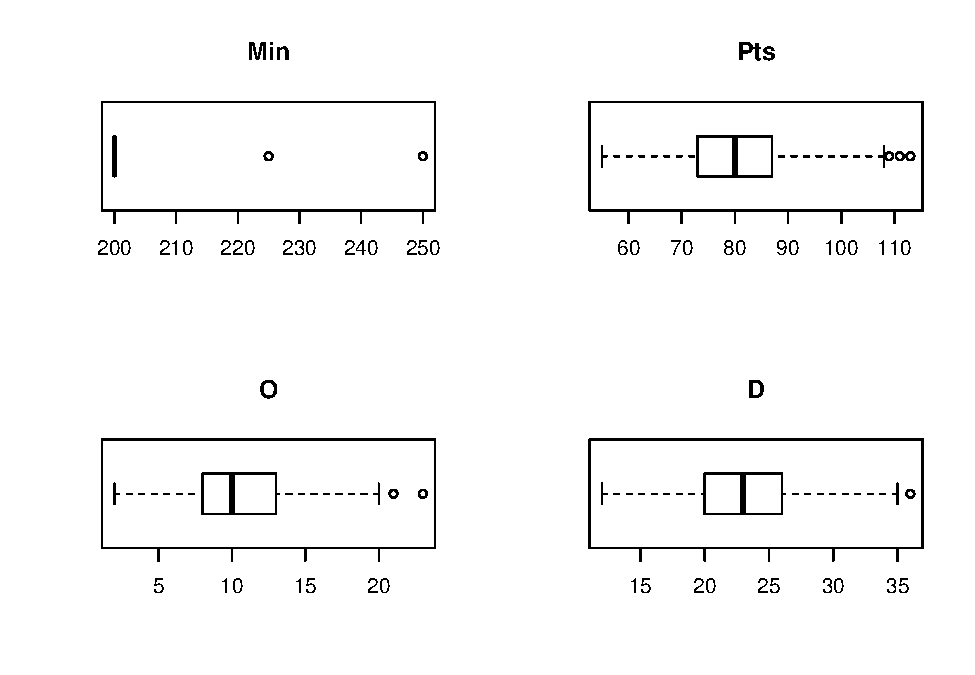
\includegraphics{practica2_files/figure-latex/unnamed-chunk-21-1.pdf}

\begin{Shaded}
\begin{Highlighting}[]
\KeywordTok{par}\NormalTok{(}\DataTypeTok{mfrow =} \KeywordTok{c}\NormalTok{(}\DecValTok{1}\NormalTok{,}\DecValTok{1}\NormalTok{))}
\end{Highlighting}
\end{Shaded}

\begin{Shaded}
\begin{Highlighting}[]
\CommentTok{# Valores extremos de la variable Min}
\NormalTok{outlier}\FloatTok{.3}\OperatorTok{$}\NormalTok{out}
\end{Highlighting}
\end{Shaded}

\begin{verbatim}
##  [1] 225 250 225 225 225 225 225 225 225 225 225 225 225 225 225 225 225 225 225
## [20] 225 225 225 250 225 225 225 225 225 225 225 225 225 225 225
\end{verbatim}

\begin{Shaded}
\begin{Highlighting}[]
\CommentTok{# Valores extremos de la variable Pts}
\NormalTok{outlier}\FloatTok{.4}\OperatorTok{$}\NormalTok{out}
\end{Highlighting}
\end{Shaded}

\begin{verbatim}
## [1] 113 109 111
\end{verbatim}

\begin{Shaded}
\begin{Highlighting}[]
\CommentTok{# Valores extremos de la variable O}
\NormalTok{outlier}\FloatTok{.5}\OperatorTok{$}\NormalTok{out}
\end{Highlighting}
\end{Shaded}

\begin{verbatim}
## [1] 21 23
\end{verbatim}

\begin{Shaded}
\begin{Highlighting}[]
\CommentTok{# Valores extremos de la variable D}
\NormalTok{outlier}\FloatTok{.6}\OperatorTok{$}\NormalTok{out}
\end{Highlighting}
\end{Shaded}

\begin{verbatim}
## [1] 36
\end{verbatim}

\newpage

\begin{Shaded}
\begin{Highlighting}[]
\KeywordTok{par}\NormalTok{(}\DataTypeTok{mfrow =} \KeywordTok{c}\NormalTok{(}\DecValTok{2}\NormalTok{,}\DecValTok{2}\NormalTok{))}
\ControlFlowTok{for}\NormalTok{ (i }\ControlFlowTok{in} \KeywordTok{c}\NormalTok{(}\KeywordTok{seq}\NormalTok{(}\DecValTok{7}\NormalTok{,}\DecValTok{10}\NormalTok{))) \{}
\NormalTok{  outlier <-}\StringTok{ }\KeywordTok{boxplot}\NormalTok{(data_team[,i], }\DataTypeTok{main =} \KeywordTok{colnames}\NormalTok{(data_team)[i], }\DataTypeTok{horizontal =} \OtherTok{TRUE}\NormalTok{)}
  \KeywordTok{assign}\NormalTok{(}\KeywordTok{paste}\NormalTok{(}\StringTok{"outlier"}\NormalTok{, i, }\DataTypeTok{sep =} \StringTok{"."}\NormalTok{), outlier)}
\NormalTok{\}}
\end{Highlighting}
\end{Shaded}

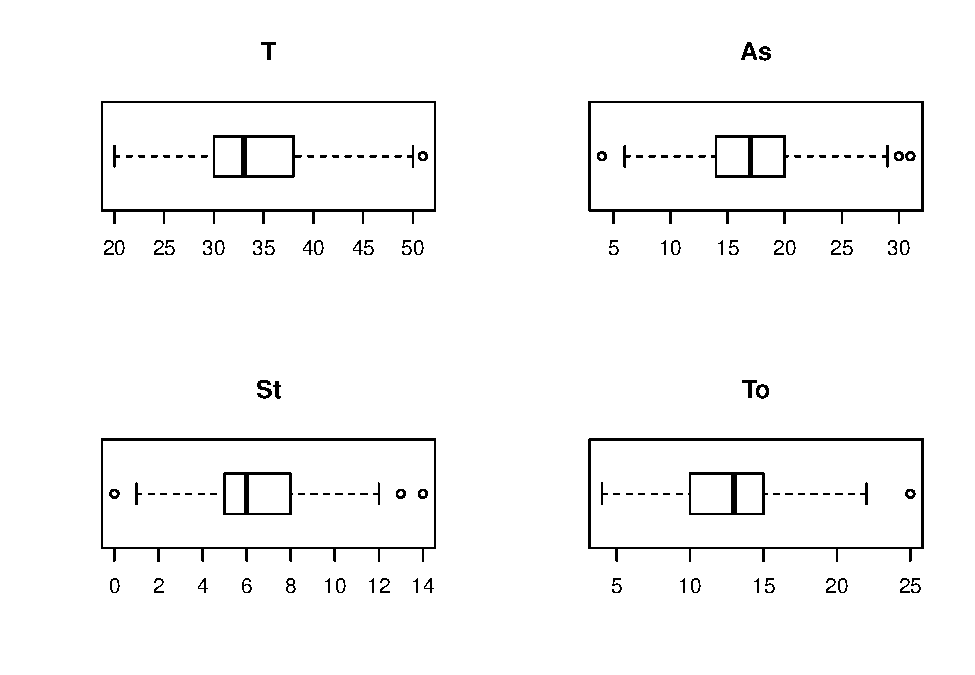
\includegraphics{practica2_files/figure-latex/unnamed-chunk-26-1.pdf}

\begin{Shaded}
\begin{Highlighting}[]
\KeywordTok{par}\NormalTok{(}\DataTypeTok{mfrow =} \KeywordTok{c}\NormalTok{(}\DecValTok{1}\NormalTok{,}\DecValTok{1}\NormalTok{))}
\end{Highlighting}
\end{Shaded}

\begin{Shaded}
\begin{Highlighting}[]
\CommentTok{# Valores extremos de la variable T}
\NormalTok{outlier}\FloatTok{.7}\OperatorTok{$}\NormalTok{out}
\end{Highlighting}
\end{Shaded}

\begin{verbatim}
## [1] 51
\end{verbatim}

\begin{Shaded}
\begin{Highlighting}[]
\CommentTok{# Valores extremos de la variable As}
\NormalTok{outlier}\FloatTok{.8}\OperatorTok{$}\NormalTok{out}
\end{Highlighting}
\end{Shaded}

\begin{verbatim}
## [1]  4 30 31 30
\end{verbatim}

\begin{Shaded}
\begin{Highlighting}[]
\CommentTok{# Valores extremos de la variable St}
\NormalTok{outlier}\FloatTok{.9}\OperatorTok{$}\NormalTok{out}
\end{Highlighting}
\end{Shaded}

\begin{verbatim}
##  [1]  0 14 14 13 13 14 14 13 13 14
\end{verbatim}

\begin{Shaded}
\begin{Highlighting}[]
\CommentTok{# Valores extremos de la variable To}
\NormalTok{outlier}\FloatTok{.10}\OperatorTok{$}\NormalTok{out}
\end{Highlighting}
\end{Shaded}

\begin{verbatim}
## [1] 25
\end{verbatim}

\newpage

\begin{Shaded}
\begin{Highlighting}[]
\KeywordTok{par}\NormalTok{(}\DataTypeTok{mfrow =} \KeywordTok{c}\NormalTok{(}\DecValTok{2}\NormalTok{,}\DecValTok{2}\NormalTok{))}
\ControlFlowTok{for}\NormalTok{ (i }\ControlFlowTok{in} \KeywordTok{c}\NormalTok{(}\KeywordTok{seq}\NormalTok{(}\DecValTok{11}\NormalTok{,}\DecValTok{14}\NormalTok{))) \{}
\NormalTok{  outlier <-}\StringTok{ }\KeywordTok{boxplot}\NormalTok{(data_team[,i], }\DataTypeTok{main =} \KeywordTok{colnames}\NormalTok{(data_team)[i], }\DataTypeTok{horizontal =} \OtherTok{TRUE}\NormalTok{)}
  \KeywordTok{assign}\NormalTok{(}\KeywordTok{paste}\NormalTok{(}\StringTok{"outlier"}\NormalTok{, i, }\DataTypeTok{sep =} \StringTok{"."}\NormalTok{), outlier)}
\NormalTok{\}}
\end{Highlighting}
\end{Shaded}

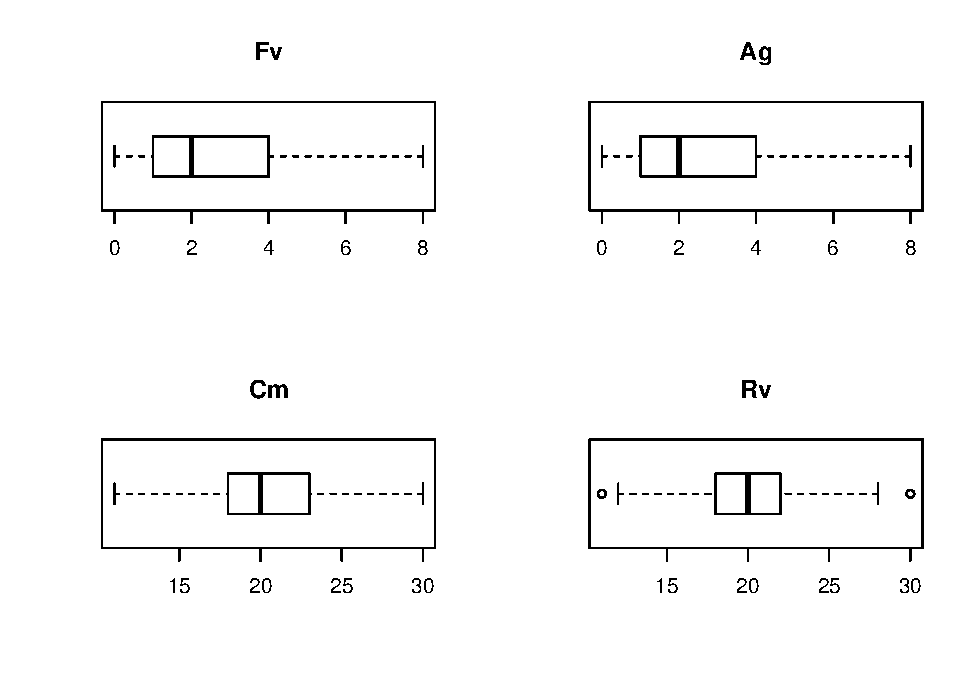
\includegraphics{practica2_files/figure-latex/unnamed-chunk-31-1.pdf}

\begin{Shaded}
\begin{Highlighting}[]
\KeywordTok{par}\NormalTok{(}\DataTypeTok{mfrow =} \KeywordTok{c}\NormalTok{(}\DecValTok{1}\NormalTok{,}\DecValTok{1}\NormalTok{))}
\end{Highlighting}
\end{Shaded}

\begin{Shaded}
\begin{Highlighting}[]
\CommentTok{# Valores extremos de la variable Rv}
\NormalTok{outlier}\FloatTok{.14}\OperatorTok{$}\NormalTok{out}
\end{Highlighting}
\end{Shaded}

\begin{verbatim}
## [1] 30 30 11 30 30 30 30
\end{verbatim}

\newpage

\begin{Shaded}
\begin{Highlighting}[]
\KeywordTok{par}\NormalTok{(}\DataTypeTok{mfrow =} \KeywordTok{c}\NormalTok{(}\DecValTok{2}\NormalTok{,}\DecValTok{2}\NormalTok{))}
\ControlFlowTok{for}\NormalTok{ (i }\ControlFlowTok{in} \KeywordTok{c}\NormalTok{(}\KeywordTok{seq}\NormalTok{(}\DecValTok{15}\NormalTok{,}\DecValTok{18}\NormalTok{))) \{}
\NormalTok{  outlier <-}\StringTok{ }\KeywordTok{boxplot}\NormalTok{(data_team[,i], }\DataTypeTok{main =} \KeywordTok{colnames}\NormalTok{(data_team)[i], }\DataTypeTok{horizontal =} \OtherTok{TRUE}\NormalTok{)}
  \KeywordTok{assign}\NormalTok{(}\KeywordTok{paste}\NormalTok{(}\StringTok{"outlier"}\NormalTok{, i, }\DataTypeTok{sep =} \StringTok{"."}\NormalTok{), outlier)}
\NormalTok{\}}
\end{Highlighting}
\end{Shaded}

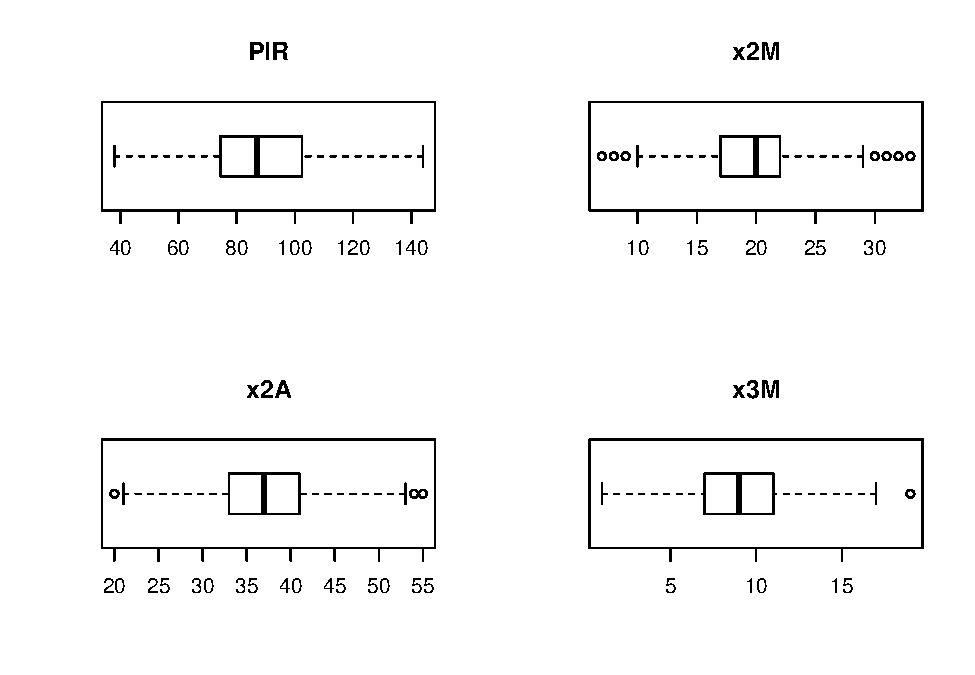
\includegraphics{practica2_files/figure-latex/unnamed-chunk-33-1.pdf}

\begin{Shaded}
\begin{Highlighting}[]
\KeywordTok{par}\NormalTok{(}\DataTypeTok{mfrow =} \KeywordTok{c}\NormalTok{(}\DecValTok{1}\NormalTok{,}\DecValTok{1}\NormalTok{))}
\end{Highlighting}
\end{Shaded}

\begin{Shaded}
\begin{Highlighting}[]
\CommentTok{# Valores extremos de la variable x2M}
\NormalTok{outlier}\FloatTok{.16}\OperatorTok{$}\NormalTok{out}
\end{Highlighting}
\end{Shaded}

\begin{verbatim}
##  [1]  8  9 33 31 32  9  7 30 30 30  7  9
\end{verbatim}

\begin{Shaded}
\begin{Highlighting}[]
\CommentTok{# Valores extremos de la variable x2A}
\NormalTok{outlier}\FloatTok{.17}\OperatorTok{$}\NormalTok{out}
\end{Highlighting}
\end{Shaded}

\begin{verbatim}
## [1] 55 20 54 55
\end{verbatim}

\begin{Shaded}
\begin{Highlighting}[]
\CommentTok{# Valores extremos de la variable x3M}
\NormalTok{outlier}\FloatTok{.18}\OperatorTok{$}\NormalTok{out}
\end{Highlighting}
\end{Shaded}

\begin{verbatim}
## [1] 19
\end{verbatim}

\newpage

\begin{Shaded}
\begin{Highlighting}[]
\KeywordTok{par}\NormalTok{(}\DataTypeTok{mfrow =} \KeywordTok{c}\NormalTok{(}\DecValTok{2}\NormalTok{,}\DecValTok{2}\NormalTok{))}
\ControlFlowTok{for}\NormalTok{ (i }\ControlFlowTok{in} \KeywordTok{c}\NormalTok{(}\KeywordTok{seq}\NormalTok{(}\DecValTok{19}\NormalTok{,}\DecValTok{21}\NormalTok{))) \{}
\NormalTok{  outlier <-}\StringTok{ }\KeywordTok{boxplot}\NormalTok{(data_team[,i], }\DataTypeTok{main =} \KeywordTok{colnames}\NormalTok{(data_team)[i], }\DataTypeTok{horizontal =} \OtherTok{TRUE}\NormalTok{)}
  \KeywordTok{assign}\NormalTok{(}\KeywordTok{paste}\NormalTok{(}\StringTok{"outlier"}\NormalTok{, i, }\DataTypeTok{sep =} \StringTok{"."}\NormalTok{), outlier)}
\NormalTok{\}}
\KeywordTok{par}\NormalTok{(}\DataTypeTok{mfrow =} \KeywordTok{c}\NormalTok{(}\DecValTok{1}\NormalTok{,}\DecValTok{1}\NormalTok{))}
\end{Highlighting}
\end{Shaded}

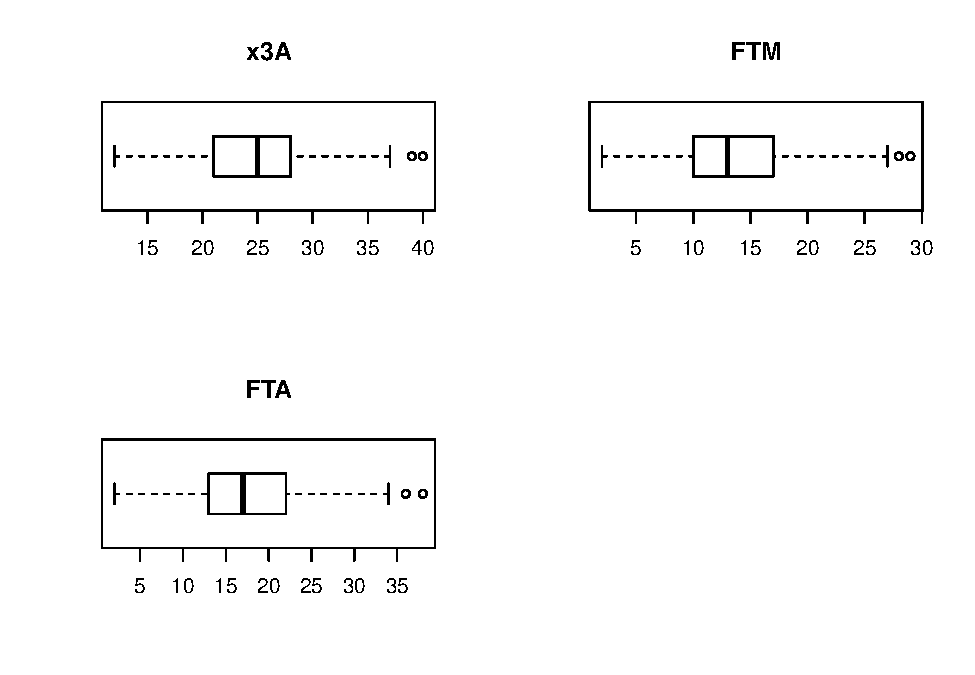
\includegraphics{practica2_files/figure-latex/unnamed-chunk-37-1.pdf}

\begin{Shaded}
\begin{Highlighting}[]
\CommentTok{# Valores extremos de la variable x3A}
\NormalTok{outlier}\FloatTok{.19}\OperatorTok{$}\NormalTok{out}
\end{Highlighting}
\end{Shaded}

\begin{verbatim}
## [1] 39 40 40 40
\end{verbatim}

\begin{Shaded}
\begin{Highlighting}[]
\CommentTok{# Valores extremos de la variable FTM}
\NormalTok{outlier}\FloatTok{.20}\OperatorTok{$}\NormalTok{out}
\end{Highlighting}
\end{Shaded}

\begin{verbatim}
## [1] 28 29 28
\end{verbatim}

\begin{Shaded}
\begin{Highlighting}[]
\CommentTok{# Valores extremos de la variable FTA}
\NormalTok{outlier}\FloatTok{.21}\OperatorTok{$}\NormalTok{out}
\end{Highlighting}
\end{Shaded}

\begin{verbatim}
## [1] 36 38 38 36
\end{verbatim}

\newpage

Mediante los gráficos de caja anteriores hemos obtenido la siguiente
información:

\begin{itemize}
\tightlist
\item
  \textbf{Variables sin \emph{outliers}:} \texttt{Fv}, \texttt{Ag},
  \texttt{Cm} y \texttt{PIR}.
\item
  \textbf{Variables con \emph{outliers}:} \texttt{Min}, \texttt{Pts},
  \texttt{O}, \texttt{D}, \texttt{T}, \texttt{As}, \texttt{St},
  \texttt{To}, \texttt{Rv}, \texttt{x2M}, \texttt{x2A}, \texttt{x3M},
  \texttt{x3A}, \texttt{FTM} y \texttt{FTA}.
\end{itemize}

Tras revisar todos individualmente todos los valores extremos hemos
determinado que todos ellos son valores posibles y que están dentro del
rango del atributo, por lo que se considerarán como valores legítimos y
se contemplarán en los análisis posteriores.

Un ejemplo claro es el de la variable que representa los minutos, donde
la mayoría de partidos duran 200 minutos con excepción de los que tienen
prórroga, como ya explicamos anteriormente cuando creamos el dataset con
las estadísticas de los equipos.

Otro ejemplo de valores extremos legítimos serían los de la variable que
representa los puntos obtenidos en un partido por un equipo: 113, 109,
111. Por lo que vemos, en la Euroliga podemos considerar como fuera de
lo habitual que un equipo meta más de 110 puntos. Si realizaramos el
mismo análisis sobre equipos de la NBA veríamos que este valor cambiaría
bastante ya que en la liga americana es más habitual que los equipos
consigan marcadores más abultados. Si hubiésemos obtenido un
\emph{outlier} de 200 o 300 para la variable puntos si hubiésemos tenido
que eliminar ese registro o revisar si se produjo un error en el proceso
de \emph{web scraping} o en la carga de datos, ya que sería un dato que
se aleja bastante de la normalidad.

\begin{center}\rule{0.5\linewidth}{0.5pt}\end{center}

\newpage

\hypertarget{enriquecimiento-de-los-datos}{%
\section{Enriquecimiento de los
datos}\label{enriquecimiento-de-los-datos}}

\hypertarget{datos-del-oponente.}{%
\subsection{Datos del oponente.}\label{datos-del-oponente.}}

Durante un encuentro de baloncesto, es tan importante medir lo que tú
equipo ha hecho como lo que tú equipo ha recibido. Por lo tanto,
buscamos enriquecer la información por partido de cada equipo añadiendo
la información del oponente. Para ello, utilizaremos el dataset
\texttt{data\_scoreboards} para completar así los registros:

\begin{Shaded}
\begin{Highlighting}[]
\KeywordTok{names}\NormalTok{(data_scoreboards)[}\KeywordTok{names}\NormalTok{(data_scoreboards) }\OperatorTok{==}\StringTok{ "Id"}\NormalTok{] <-}\StringTok{ "MatchId"}
\KeywordTok{names}\NormalTok{(data_scoreboards)[}\KeywordTok{names}\NormalTok{(data_scoreboards) }\OperatorTok{==}\StringTok{ "HomeTeam"}\NormalTok{] <-}\StringTok{ "Team"}
\KeywordTok{names}\NormalTok{(data_scoreboards)[}\KeywordTok{names}\NormalTok{(data_scoreboards) }\OperatorTok{==}\StringTok{ "VisitingTeam"}\NormalTok{] <-}\StringTok{ "Opponent"}

\NormalTok{df_}\DecValTok{1}\NormalTok{ <-}\StringTok{ }\KeywordTok{merge}\NormalTok{(data_team, data_scoreboards, }\DataTypeTok{by=}\KeywordTok{c}\NormalTok{(}\StringTok{"MatchId"}\NormalTok{,}\StringTok{"Team"}\NormalTok{))}
\NormalTok{df_}\DecValTok{1}\NormalTok{[}\StringTok{"Local"}\NormalTok{] <-}\StringTok{ }\DecValTok{1}

\KeywordTok{names}\NormalTok{(data_scoreboards)[}\KeywordTok{names}\NormalTok{(data_scoreboards) }\OperatorTok{==}\StringTok{ "Team"}\NormalTok{] <-}\StringTok{ "HomeTeam"}
\KeywordTok{names}\NormalTok{(data_scoreboards)[}\KeywordTok{names}\NormalTok{(data_scoreboards) }\OperatorTok{==}\StringTok{ "Opponent"}\NormalTok{] <-}\StringTok{ "Team"}
\KeywordTok{names}\NormalTok{(data_scoreboards)[}\KeywordTok{names}\NormalTok{(data_scoreboards) }\OperatorTok{==}\StringTok{ "HomeTeam"}\NormalTok{] <-}\StringTok{ "Opponent"}
\NormalTok{df_}\DecValTok{2}\NormalTok{ <-}\StringTok{ }\KeywordTok{merge}\NormalTok{(data_team, data_scoreboards, }\DataTypeTok{by=}\KeywordTok{c}\NormalTok{(}\StringTok{"MatchId"}\NormalTok{,}\StringTok{"Team"}\NormalTok{))}
\NormalTok{df_}\DecValTok{2}\NormalTok{[}\StringTok{"Local"}\NormalTok{] <-}\StringTok{ }\DecValTok{0}

\NormalTok{data_team <-}\StringTok{ }\KeywordTok{bind_rows}\NormalTok{(df_}\DecValTok{1}\NormalTok{,df_}\DecValTok{2}\NormalTok{)}

\NormalTok{data_team[}\KeywordTok{c}\NormalTok{(}\StringTok{"Date"}\NormalTok{)] <-}\StringTok{ }\OtherTok{NULL}
\NormalTok{data_team[}\KeywordTok{c}\NormalTok{(}\StringTok{"HomeScore"}\NormalTok{)] <-}\StringTok{ }\OtherTok{NULL}
\NormalTok{data_team[}\KeywordTok{c}\NormalTok{(}\StringTok{"VisitingScore"}\NormalTok{)] <-}\StringTok{ }\OtherTok{NULL}
\NormalTok{data_team[}\KeywordTok{c}\NormalTok{(}\StringTok{"Link"}\NormalTok{)] <-}\StringTok{ }\OtherTok{NULL}

\NormalTok{data_team2 <-}\StringTok{ }\NormalTok{data_team [}\KeywordTok{c}\NormalTok{(}\StringTok{"MatchId"}\NormalTok{,}\StringTok{"Team"}\NormalTok{,}\StringTok{"Min"}\NormalTok{,}\StringTok{"Pts"}\NormalTok{,}\StringTok{"O"}\NormalTok{,}\StringTok{"D"}\NormalTok{,}\StringTok{"T"}\NormalTok{,}\StringTok{"As"}\NormalTok{,}\StringTok{"St"}\NormalTok{,}\StringTok{"To"}\NormalTok{,}
                           \StringTok{"Fv"}\NormalTok{,}\StringTok{"Ag"}\NormalTok{,}\StringTok{"Cm"}\NormalTok{,}\StringTok{"Rv"}\NormalTok{,}\StringTok{"PIR"}\NormalTok{,}\StringTok{"x2M"}\NormalTok{,}\StringTok{"x2A"}\NormalTok{,}\StringTok{"x3M"}\NormalTok{,}\StringTok{"x3A"}\NormalTok{,}\StringTok{"FTM"}\NormalTok{,}
                           \StringTok{"FTA"}\NormalTok{)]}

\KeywordTok{names}\NormalTok{(data_team2)[}\KeywordTok{names}\NormalTok{(data_team2) }\OperatorTok{==}\StringTok{ "Pts"}\NormalTok{] <-}\StringTok{ "Pts_Opp"}
\KeywordTok{names}\NormalTok{(data_team2)[}\KeywordTok{names}\NormalTok{(data_team2) }\OperatorTok{==}\StringTok{ "O"}\NormalTok{] <-}\StringTok{ "O_Opp"}
\KeywordTok{names}\NormalTok{(data_team2)[}\KeywordTok{names}\NormalTok{(data_team2) }\OperatorTok{==}\StringTok{ "D"}\NormalTok{] <-}\StringTok{ "D_Opp"}
\KeywordTok{names}\NormalTok{(data_team2)[}\KeywordTok{names}\NormalTok{(data_team2) }\OperatorTok{==}\StringTok{ "T"}\NormalTok{] <-}\StringTok{ "T_Opp"}
\KeywordTok{names}\NormalTok{(data_team2)[}\KeywordTok{names}\NormalTok{(data_team2) }\OperatorTok{==}\StringTok{ "As"}\NormalTok{] <-}\StringTok{ "As_Opp"}
\KeywordTok{names}\NormalTok{(data_team2)[}\KeywordTok{names}\NormalTok{(data_team2) }\OperatorTok{==}\StringTok{ "St"}\NormalTok{] <-}\StringTok{ "St_Opp"}
\KeywordTok{names}\NormalTok{(data_team2)[}\KeywordTok{names}\NormalTok{(data_team2) }\OperatorTok{==}\StringTok{ "To"}\NormalTok{] <-}\StringTok{ "To_Opp"}
\KeywordTok{names}\NormalTok{(data_team2)[}\KeywordTok{names}\NormalTok{(data_team2) }\OperatorTok{==}\StringTok{ "Fv"}\NormalTok{] <-}\StringTok{ "Fv_Opp"}
\KeywordTok{names}\NormalTok{(data_team2)[}\KeywordTok{names}\NormalTok{(data_team2) }\OperatorTok{==}\StringTok{ "Ag"}\NormalTok{] <-}\StringTok{ "Ag_Opp"}
\KeywordTok{names}\NormalTok{(data_team2)[}\KeywordTok{names}\NormalTok{(data_team2) }\OperatorTok{==}\StringTok{ "Cm"}\NormalTok{] <-}\StringTok{ "Cm_Opp"}
\KeywordTok{names}\NormalTok{(data_team2)[}\KeywordTok{names}\NormalTok{(data_team2) }\OperatorTok{==}\StringTok{ "Rv"}\NormalTok{] <-}\StringTok{ "Rv_Opp"}
\KeywordTok{names}\NormalTok{(data_team2)[}\KeywordTok{names}\NormalTok{(data_team2) }\OperatorTok{==}\StringTok{ "PIR"}\NormalTok{] <-}\StringTok{ "PIR_Opp"}
\KeywordTok{names}\NormalTok{(data_team2)[}\KeywordTok{names}\NormalTok{(data_team2) }\OperatorTok{==}\StringTok{ "x2M"}\NormalTok{] <-}\StringTok{ "x2M_Opp"}
\KeywordTok{names}\NormalTok{(data_team2)[}\KeywordTok{names}\NormalTok{(data_team2) }\OperatorTok{==}\StringTok{ "x2A"}\NormalTok{] <-}\StringTok{ "x2A_Opp"}
\KeywordTok{names}\NormalTok{(data_team2)[}\KeywordTok{names}\NormalTok{(data_team2) }\OperatorTok{==}\StringTok{ "x3M"}\NormalTok{] <-}\StringTok{ "x3M_Opp"}
\KeywordTok{names}\NormalTok{(data_team2)[}\KeywordTok{names}\NormalTok{(data_team2) }\OperatorTok{==}\StringTok{ "x3A"}\NormalTok{] <-}\StringTok{ "x3A_Opp"}
\KeywordTok{names}\NormalTok{(data_team2)[}\KeywordTok{names}\NormalTok{(data_team2) }\OperatorTok{==}\StringTok{ "FTM"}\NormalTok{] <-}\StringTok{ "FTM_Opp"}
\KeywordTok{names}\NormalTok{(data_team2)[}\KeywordTok{names}\NormalTok{(data_team2) }\OperatorTok{==}\StringTok{ "FTA"}\NormalTok{] <-}\StringTok{ "FTA_Opp"}

\NormalTok{data_teamopp <-}\StringTok{ }\KeywordTok{merge}\NormalTok{(data_team, data_team2, }\DataTypeTok{by.x=}\KeywordTok{c}\NormalTok{(}\StringTok{"MatchId"}\NormalTok{,}\StringTok{"Opponent"}\NormalTok{),  }
                      \DataTypeTok{by.y=}\KeywordTok{c}\NormalTok{(}\StringTok{"MatchId"}\NormalTok{,}\StringTok{"Team"}\NormalTok{))}
\NormalTok{data_teamopp[}\StringTok{"y.min"}\NormalTok{]<-}\OtherTok{NULL}
\end{Highlighting}
\end{Shaded}

\newpage

\hypertarget{creaciuxf3n-de-nuevas-muxe9tricas-de-equipo}{%
\subsection{Creación de nuevas métricas de
equipo}\label{creaciuxf3n-de-nuevas-muxe9tricas-de-equipo}}

Durante los últimos años, se ha dado una vuelta al análisis de la
estadísticas en baloncesto. Como los diferentes equipos, de acuerdo a su
estilo, juegan a distintos ritmos, no podemos usar los promedios por
partido para compararlos. Para poder lograr las comparaciones hay
definir el concepto de las posesiones, que es la base de estos cálculos.
El basket es un juego en el que ambos equipos se alternan la posesión de
la pelota. El equipo que aproveche mejor sus posesiones será el equipo
ganador. Se entiende que una posesión termina con un tiro al aro, una
pérdida de balón o un tiro libre. Allí el balón pasa al rival y la
posesión se termina. ¿Qué ocurre si el equipo falla el tiro de campo
pero captura el rebote ofensivo? Hoy por hoy, la mayoría de los
estadistas de baloncesto consideran que no se le debe anotar una nueva
posesión al equipo, sino considerar que la misma posesión continúa.

Para tener en cuenta lo anteriormente mencionado, a continuación
definiremos nuevas métricas.

\hypertarget{ritmo-pace}{%
\subsubsection{Ritmo (Pace)}\label{ritmo-pace}}

Nos da una idea del ritmo de juego del equipo, expresado en cantidad de
posesiones por juego que utiliza. Hay equipos que corren más y equipos
que prefieren el juego estático. Por eso las estadísticas por juego no
sirven para comparar equipos. Las posesiones se calculan con la
siguiente fórmula:

\[
  \makebox[\linewidth]{$Pos = FGA - OR + TO + (FTA*0.4)$}
\]

Donde:

\begin{itemize}
\tightlist
\item
  Pos: posesiones
\item
  FGA (field goal attempts): lanzamientos de campo (tanto de 2 y de 3)
\item
  OR (ofensive rebounds): rebotes ofensivos
\item
  TO (turnovers): pelotas perdidas
\item
  FTA (free throw attempts): tiros libres lanzados \newline
\end{itemize}

\begin{Shaded}
\begin{Highlighting}[]
\NormalTok{data_teamopp[}\StringTok{"Poss"}\NormalTok{] <-}\StringTok{ }\NormalTok{data_teamopp[}\StringTok{"x2A"}\NormalTok{] }\OperatorTok{+}\StringTok{ }\NormalTok{data_teamopp[}\StringTok{"x3A"}\NormalTok{] }\OperatorTok{-}\StringTok{ }
\StringTok{  }\NormalTok{data_teamopp[}\StringTok{"O"}\NormalTok{] }\OperatorTok{+}\StringTok{ }\NormalTok{data_teamopp[}\StringTok{"To"}\NormalTok{] }\OperatorTok{+}\StringTok{ }\NormalTok{(}\FloatTok{0.4}\OperatorTok{*}\NormalTok{data_teamopp[}\StringTok{"FTA"}\NormalTok{])}
\end{Highlighting}
\end{Shaded}

\hypertarget{eficiencia-ofensiva-rating-ofensivo}{%
\subsubsection{Eficiencia ofensiva (Rating
ofensivo)}\label{eficiencia-ofensiva-rating-ofensivo}}

Habitualmente se evalúa la ofensiva en puntos convertidos por juego, lo
cual es una manera un tanto absurda. Si pensamos el juego como una serie
de posesiones, el equipo que más puntos convierta en sus posesiones,
será el más efectivo. Se multiplica por 100 para expresar los puntos
cada 100 posesiones, y no manejar números con decimales. Así:

\[
  \makebox[\linewidth]{$Offensive Rating = (puntos/posesiones)*100$}
\]

\begin{Shaded}
\begin{Highlighting}[]
\NormalTok{data_teamopp [}\StringTok{"Off_Rat"}\NormalTok{] <-}\StringTok{ }\OperatorTok{+}\NormalTok{data_teamopp[}\StringTok{"Pts"}\NormalTok{]}\OperatorTok{/}\NormalTok{data_teamopp[}\StringTok{"Poss"}\NormalTok{]}
\end{Highlighting}
\end{Shaded}

\newpage

\hypertarget{eficiencia-defensiva-rating-defensivo}{%
\subsubsection{Eficiencia defensiva (Rating
defensivo)}\label{eficiencia-defensiva-rating-defensivo}}

Así como medimos la eficiencia ofensiva en base a puntos convertidos
cada 100 posesiones, podemos medir la defensa en base a puntos recibidos
(o puntos del oponente) cada 100 posesiones del equipo contrario.

\[
  \makebox[\linewidth]{$Defensive Rating = (puntos_{oponente}/posesiones)*100$}
\]

\begin{Shaded}
\begin{Highlighting}[]
\NormalTok{data_teamopp [}\StringTok{"Def_Rat"}\NormalTok{] <-}\StringTok{ }\OperatorTok{+}\NormalTok{data_teamopp[}\StringTok{"Pts_Opp"}\NormalTok{]}\OperatorTok{/}\NormalTok{data_teamopp[}\StringTok{"Poss"}\NormalTok{]}
\end{Highlighting}
\end{Shaded}

\hypertarget{porcentaje-efectivo-de-tiros-de-campo-efg}{%
\subsubsection{Porcentaje efectivo de tiros de campo
(eFG\%)}\label{porcentaje-efectivo-de-tiros-de-campo-efg}}

Esta estadística ajusta los tiros de campo dandole el valor extra (un
punto más) a los triples. Esto corrige el FG\% común que subestima a los
triples. Por ejemplo, si un jugador ha hecho 2/5 en T2 y 1/4 en T3,
habrá convertido 3/9 en tiros de campo (33\%), que es similar a si
hubiera metido 3/5 de T2 y 0/4 en T3. Sin embargo, en el primer supuesto
ha conseguido más puntos para el equipo. Así, el eFG\% del primero será
44.4\% que se ajusta más a la realidad. La fórmula, por tanto es:

\[
  \makebox[\linewidth]{$eFG\% = \frac{(FGM + 0.5*3PM)}{FGA}$}
\]

Donde:

\begin{itemize}
\tightlist
\item
  FGM (field goal made): tiros de campo convertidos.
\item
  3PM (3 points made): triples convertidos.
\item
  FGA (field goal attempts): tiros de campo intentados.
\end{itemize}

\begin{Shaded}
\begin{Highlighting}[]
\NormalTok{data_teamopp [}\StringTok{"eFG"}\NormalTok{] <-}\StringTok{ }\NormalTok{(data_teamopp[}\StringTok{"x2M"}\NormalTok{] }\OperatorTok{+}\StringTok{ }\FloatTok{1.5}\OperatorTok{*}\NormalTok{data_teamopp[}\StringTok{"x3M"}\NormalTok{]) }\OperatorTok{/}
\StringTok{  }\NormalTok{(data_teamopp[}\StringTok{"x2A"}\NormalTok{] }\OperatorTok{+}\StringTok{ }\NormalTok{data_teamopp[}\StringTok{"x3A"}\NormalTok{])}

\NormalTok{data_teamopp [}\StringTok{"eFG_Opp"}\NormalTok{] <-}\StringTok{ }\NormalTok{(data_teamopp[}\StringTok{"x2M_Opp"}\NormalTok{] }\OperatorTok{+}\StringTok{ }\FloatTok{1.5}\OperatorTok{*}\NormalTok{data_teamopp[}\StringTok{"x3M_Opp"}\NormalTok{]) }\OperatorTok{/}
\StringTok{  }\NormalTok{(data_teamopp[}\StringTok{"x2A_Opp"}\NormalTok{]}\OperatorTok{+}\NormalTok{data_teamopp[}\StringTok{"x3A_Opp"}\NormalTok{])}
\end{Highlighting}
\end{Shaded}

\hypertarget{lanzamientos-reales-true-shooting}{%
\subsubsection{Lanzamientos reales (True
Shooting)}\label{lanzamientos-reales-true-shooting}}

Esta métrica tiene en cuenta los dobles, triples y tiros libres, para
dar una idea de cómo tira el jugador globalmente. Ejemplo: en la
2009-2010, Martin Leiva quedó \#8 en FG\% con 58,72. Pero si le
agregamos los libres, cae al puesto \#91 con 54.8\%. La fórmula es:

\[
  \makebox[\linewidth]{$TS = \frac{puntos}{2*(FGA+0.44*FTA)}$}
\]

Donde:

\begin{itemize}
\tightlist
\item
  FGA (field goal attempts): lanzamientos de cancha intentados
\item
  FTA (free throw attempts): tiros libres intentados
\end{itemize}

\begin{Shaded}
\begin{Highlighting}[]
\NormalTok{data_teamopp [}\StringTok{"TS"}\NormalTok{] <-}\StringTok{ }\NormalTok{data_teamopp[}\StringTok{"Pts"}\NormalTok{] }\OperatorTok{/}
\StringTok{  }\NormalTok{(data_teamopp[}\StringTok{"x2A"}\NormalTok{] }\OperatorTok{+}\StringTok{ }\NormalTok{data_teamopp[}\StringTok{"x3A"}\NormalTok{] }\OperatorTok{+}\StringTok{ }\FloatTok{0.44}\OperatorTok{*}\NormalTok{data_teamopp[}\StringTok{"FTA"}\NormalTok{])}

\NormalTok{data_teamopp [}\StringTok{"TS_Opp"}\NormalTok{] <-}\StringTok{ }\NormalTok{data_teamopp[}\StringTok{"Pts_Opp"}\NormalTok{] }\OperatorTok{/}
\StringTok{  }\NormalTok{(data_teamopp[}\StringTok{"x2A_Opp"}\NormalTok{] }\OperatorTok{+}\StringTok{ }\NormalTok{data_teamopp[}\StringTok{"x3A_Opp"}\NormalTok{] }\OperatorTok{+}\StringTok{ }\FloatTok{0.44}\OperatorTok{*}\NormalTok{data_teamopp[}\StringTok{"FTA_Opp"}\NormalTok{])}
\end{Highlighting}
\end{Shaded}

\newpage

\hypertarget{rebotes}{%
\subsubsection{Rebotes}\label{rebotes}}

Los rebotes totales de un equipo son de poco valor. Capturar un rebote
ofensivo requiere diferentes habilidades que capturar uno defensivo, por
lo que deben analizarse por separado.

Tener en cuenta el número absoluto de rebotes conseguidos, o el promedio
de rebotes por partido, nos puede llevar a errores, ya que los rebotes
disponibles dependen de la efectividad: si un equipo falla poco, hay
pocos rebotes por tomar.

Ejemplo: el equipo A obtuvo en un partido 20 rebotes defensivos. Si el
equipo B falló 30 lanzamientos (o sea que hubo 30 rebotes en el aro
defensivo de A) entonces A capturó 66\% de los rebotes en su aro (20 de
30). Pero si B erró 25 tiros, A tomó 80\% de los rebotes (20 de 25).

Esto hace que, para evaluarlo correctamente, definamos: DR\% como
porcentaje de rebotes defensivos y OR\% porcentaje de rebotes ofensivos.

\hypertarget{tasa-de-rebotes-ofensivos}{%
\paragraph{Tasa de rebotes ofensivos}\label{tasa-de-rebotes-ofensivos}}

\[
  \makebox[\linewidth]{$\% de rebotes ofensivos = [OR/(OR+op DR)]*100$}
\]

Donde:

\begin{itemize}
\tightlist
\item
  OR (ofensive rebounds): rebotes ofensivos.
\item
  Op DR (oponent defensive rebounds): rebotes defensivos del rival.
\end{itemize}

\hypertarget{tasa-de-rebotes-defensivos}{%
\paragraph{Tasa de rebotes
defensivos}\label{tasa-de-rebotes-defensivos}}

\[
  \makebox[\linewidth]{$\% de rebotes defensivos = [DR/(DR+op OR)]*100$}
\]

Donde:

\begin{itemize}
\tightlist
\item
  DR (defensive rebounds): rebotes defensivos.
\item
  Op OR (oponent ofensive rebounds): rebotes ofensivos del rival.
\end{itemize}

\begin{Shaded}
\begin{Highlighting}[]
\NormalTok{data_teamopp [}\StringTok{"Off_Reb"}\NormalTok{] <-}\StringTok{ }\NormalTok{data_teamopp[}\StringTok{"O"}\NormalTok{] }\OperatorTok{/}\StringTok{  }\NormalTok{(data_teamopp[}\StringTok{"O"}\NormalTok{]}\OperatorTok{+}\NormalTok{data_teamopp[}\StringTok{"D_Opp"}\NormalTok{])}

\NormalTok{data_teamopp [}\StringTok{"Def_Reb"}\NormalTok{] <-}\StringTok{ }\NormalTok{data_teamopp[}\StringTok{"D"}\NormalTok{] }\OperatorTok{/}\StringTok{  }\NormalTok{(data_teamopp[}\StringTok{"D"}\NormalTok{]}\OperatorTok{+}\NormalTok{data_teamopp[}\StringTok{"O_Opp"}\NormalTok{])}
\end{Highlighting}
\end{Shaded}

\hypertarget{porcentaje-de-asistencias-y-puxe9rdidas}{%
\subsubsection{Porcentaje de asistencias y
pérdidas}\label{porcentaje-de-asistencias-y-puxe9rdidas}}

Al igual que con los rebotes y otras estadísitcas, las asistencias por
juego no son un buen parámetro, ya que dependen del ritmo de juego. Es
más preciso calcular las asistencias expresadas en posesiones terminan
con una pérdida de balón. Habitualmente expresado en porcentaje.

\hypertarget{porcentaje-de-asistencias}{%
\subsubsection{Porcentaje de
asistencias}\label{porcentaje-de-asistencias}}

Se calculan mediante la siguiente fórmula:

\[
  \makebox[\linewidth]{$\% de asistencias = (asistencias/posesiones)*100$}
\]

\begin{Shaded}
\begin{Highlighting}[]
\NormalTok{data_teamopp [}\StringTok{"Pct_ass"}\NormalTok{] <-}\StringTok{ }\NormalTok{data_teamopp[}\StringTok{"As"}\NormalTok{] }\OperatorTok{/}\StringTok{  }\NormalTok{(data_teamopp[}\StringTok{"Poss"}\NormalTok{])}

\NormalTok{data_teamopp [}\StringTok{"Pct_ass_opp"}\NormalTok{] <-}\StringTok{ }\NormalTok{data_teamopp[}\StringTok{"As_Opp"}\NormalTok{] }\OperatorTok{/}\StringTok{  }\NormalTok{(data_teamopp[}\StringTok{"Poss"}\NormalTok{])}
\end{Highlighting}
\end{Shaded}

\newpage

\hypertarget{porcentaje-de-puxe9rdidas}{%
\paragraph{Porcentaje de pérdidas}\label{porcentaje-de-puxe9rdidas}}

Lo mismo ocurre con las pérdidas. No es lo mismo perder 10 pelotas en un
partido en que hubo 100 posesiones, que en uno que hubo 80. Por eso es
mejor calcular las pérdidas cada 100 posesiones. El valor ideal depende
del ritmo de juego, pero podríamos decir que el objetivo sería tener
menos de 15\% de TO y provocar en el oponente más de 15\%. La fórmula
es:

\[
  \makebox[\linewidth]{$\% de pérdidas = (pelotas pérdidas/posesiones)*100$}
\]

\begin{Shaded}
\begin{Highlighting}[]
\NormalTok{data_teamopp [}\StringTok{"Pct_To"}\NormalTok{] <-}\StringTok{ }\NormalTok{data_teamopp[}\StringTok{"To"}\NormalTok{] }\OperatorTok{/}\StringTok{  }\NormalTok{(data_teamopp[}\StringTok{"Poss"}\NormalTok{])}

\NormalTok{data_teamopp [}\StringTok{"Pct_To_opp"}\NormalTok{] <-}\StringTok{ }\NormalTok{data_teamopp[}\StringTok{"To_Opp"}\NormalTok{] }\OperatorTok{/}\StringTok{  }\NormalTok{(data_teamopp[}\StringTok{"Poss"}\NormalTok{])}
\end{Highlighting}
\end{Shaded}

\hypertarget{tiros-libres-respecto-a-tiros-de-campo-ftmfga}{%
\paragraph{Tiros libres, respecto a tiros de campo
(FTM/FGA)}\label{tiros-libres-respecto-a-tiros-de-campo-ftmfga}}

Es simplemente una manera de expresar el número de veces que un equipo
va a la línea y cuántas veces envía al oponente a la línea. Esta
considerado (junto con el \emph{effective field goal percentage}, la
tasa de rebotes ofensivos y la tasa de pérdidas) uno de los cuatro
factores con los que se miden los partidos. La fórmula es:

\[
  \makebox[\linewidth]{$Libres por lanzamientos de cancha = (libres convertidos/tiros de cancha intentados) * 100$}
\]

\begin{Shaded}
\begin{Highlighting}[]
\NormalTok{data_teamopp[}\StringTok{"FTR"}\NormalTok{] <-}\StringTok{ }\NormalTok{data_teamopp[}\StringTok{"FTM"}\NormalTok{] }\OperatorTok{/}\StringTok{  }\NormalTok{(data_teamopp[}\StringTok{"x2A"}\NormalTok{]}\OperatorTok{+}\StringTok{ }\NormalTok{data_teamopp[}\StringTok{"x3A"}\NormalTok{])}

\NormalTok{data_teamopp[}\StringTok{"FTR_opp"}\NormalTok{] <-}\StringTok{ }\NormalTok{data_teamopp[}\StringTok{"FTM_Opp"}\NormalTok{] }\OperatorTok{/}
\StringTok{  }\NormalTok{(data_teamopp[}\StringTok{"x2A_Opp"}\NormalTok{]}\OperatorTok{+}\StringTok{ }\NormalTok{data_teamopp[}\StringTok{"x3A_Opp"}\NormalTok{])}
\end{Highlighting}
\end{Shaded}

\hypertarget{victoria}{%
\subsubsection{Victoria}\label{victoria}}

Otro aspecto fundamental en un partido de baloncesto y que necesitaremos
para realizar los análisis es saber quién ganó el partido. Esto se puede
obtener simplemente comparando el resultado final y determinando quién
metió más puntos:

\begin{Shaded}
\begin{Highlighting}[]
\NormalTok{data_teamopp}\OperatorTok{$}\NormalTok{Win <-}\StringTok{ }\KeywordTok{ifelse}\NormalTok{(data_teamopp}\OperatorTok{$}\NormalTok{Pts}\OperatorTok{>=}\NormalTok{data_teamopp}\OperatorTok{$}\NormalTok{Pts_Opp, }\DecValTok{1}\NormalTok{, }\DecValTok{0}\NormalTok{) }
\end{Highlighting}
\end{Shaded}

\hypertarget{triunfos-esperados-expected-wins}{%
\subsubsection{Triunfos esperados (Expected
wins)}\label{triunfos-esperados-expected-wins}}

Para ganar, obviamente hay que meter más puntos que el rival. Existe un
cálculo (comprobado en la NBA, baloncesto FIBA y universitario) que de
acuerdo a los puntos convertidos y recibidos, se puede estimar la
cantidad de partidos que habría que haber ganado. Suele correlacionar
muy bien con la realidad.

\[
  \makebox[\linewidth]{$Triunfos esperados = eficiencia ofensiva^{14}/(eficiencia ofensiva^{14}+eficiencia defensiva^{14})$}
\]

\begin{Shaded}
\begin{Highlighting}[]
\NormalTok{data_teamopp [}\StringTok{"Expected_Wins"}\NormalTok{] <-}\StringTok{ }\NormalTok{data_teamopp[}\StringTok{"Off_Rat"}\NormalTok{]}\OperatorTok{^}\DecValTok{14} \OperatorTok{/}
\StringTok{  }\NormalTok{(data_teamopp[}\StringTok{"Off_Rat"}\NormalTok{]}\OperatorTok{^}\DecValTok{14}\OperatorTok{+}\NormalTok{data_teamopp[}\StringTok{"Def_Rat"}\NormalTok{]}\OperatorTok{^}\DecValTok{14}\NormalTok{)}
\end{Highlighting}
\end{Shaded}

\newpage

\hypertarget{creaciuxf3n-de-nuevas-muxe9tricas-de-jugadores}{%
\subsection{Creación de nuevas métricas de
jugadores}\label{creaciuxf3n-de-nuevas-muxe9tricas-de-jugadores}}

Una vez definidas los nuevos estadísticos para el dataset de equipos,
realizaremos el mismo trabajo para el dataset de jugadores. De esta
forma contaremos con nuevas variables que permitan determinar con mayor
precisión la calidad y participación de los jugadores en un partido.

Para obtener estos estadísticos nos hemos basado en un artículo de la
página web \textbf{Bleacher Report} donde se explican métricas y
estadísticas avanzadas para la NBA. Se puede acceder al artículo
haciendo
\href{https://bleacherreport.com/articles/1039116-understanding-the-nba-explaining-advanced-offensive-stats-and-metrics}{\textcolor{blue}{click aquí}}.

Como necesitaremos datos del equipo, de nuevo el primer paso es
enriquecer la tabla cruzando los datos de players y de equipos por
partidos.

\begin{Shaded}
\begin{Highlighting}[]
\NormalTok{data_players <-}\StringTok{ }\KeywordTok{merge}\NormalTok{(data_euroleague, data_teamopp, }\DataTypeTok{by=}\KeywordTok{c}\NormalTok{(}\StringTok{"MatchId"}\NormalTok{,}\StringTok{"Team"}\NormalTok{))}
\end{Highlighting}
\end{Shaded}

\hypertarget{assist-percentage-ast}{%
\subsubsection{Assist Percentage (AST\%)}\label{assist-percentage-ast}}

\[
  \makebox[\linewidth]{$A/(((MP/(TMP/5))*TFG)-FG)$}
\]

Donde:

\begin{itemize}
\tightlist
\item
  A: Asistencias.
\item
  MP: Minutos jugados por el jugador.
\item
  TMP: Minutos jugados por el equipo.
\item
  TFG: Tiros de campo del equipo.
\item
  FG: Tiros de campo del jugador.
\end{itemize}

\textbf{Explicación}

Si bien las asistencias en sí mismas son bastante útiles para observar,
el porcentaje de asistencias es una estadística mucho mejor para
describir la habilidad del jugador. Las estadísticas de asistencia se
pueden completar de dos maneras: la cantidad de tiempo que un jugador
está en la cancha y el ritmo al que juega su equipo.

Un jugador en un equipo de ritmo rápido como Miami Heat o Washington
Wizards tendrá más oportunidades ofensivas para acumular asistencias, lo
que generará un mayor número de asistencias por partido y por minuto.

Del mismo modo, un jugador que juega 35 minutos por juego tendrá más
oportunidades de generar asistencias que un jugador en la cancha durante
20 minutos por partido. Puede parecer de sentido común que promediar 10
asistencias por juego en 20 minutos de acción por competencia es más
impresionante que promediar 10 asistencias por juego en 35 minutos de
acción por competencia, pero esa distinción se pierde cuando solo se
citan asistencias por partido.

La métrica esencialmente estima (estima, no calcula) qué porcentaje de
tiros realizados por los compañeros de equipo fueron asistidos por un
jugador mientras estaba en la cancha.

\textbf{Limitaciones}

Sin tener el detalle de las jugadas por partido, lo mejor que puede
hacer esta estadística es proporcionar una estimación del porcentaje
antes mencionado. No hay forma de medir y dar crédito a los buenos pases
que resultaron en tiros liberados pero fallados o pérdidas por parte del
receptor.

Al igual que con cualquier estadística de asistencia, un jugador está a
merced de la habilidad de sus compañeros de equipo.

\begin{Shaded}
\begin{Highlighting}[]
\NormalTok{data_players}\OperatorTok{$}\NormalTok{Assist_pct <-}\StringTok{ }\NormalTok{data_players}\OperatorTok{$}\NormalTok{As.x}\OperatorTok{/}\NormalTok{(((data_players}\OperatorTok{$}\NormalTok{Min}\OperatorTok{/}\NormalTok{(data_players}\OperatorTok{$}\NormalTok{Min.x}\OperatorTok{/}\DecValTok{5}\NormalTok{))}\OperatorTok{*}
\StringTok{                                                 }\NormalTok{(data_players}\OperatorTok{$}\NormalTok{x2A.y}\OperatorTok{+}\NormalTok{data_players}\OperatorTok{$}\NormalTok{x3A.y))}\OperatorTok{-}
\StringTok{                                                }\NormalTok{(data_players}\OperatorTok{$}\NormalTok{x2A.x}\OperatorTok{+}\NormalTok{data_players}\OperatorTok{$}\NormalTok{x3A.x))}
\end{Highlighting}
\end{Shaded}

\hypertarget{turnover-percentage-tov}{%
\subsubsection{Turnover Percentage
(TOV\%)}\label{turnover-percentage-tov}}

\[
  \makebox[\linewidth]{$100*TO/(FGA+0.44*FTA+TO)$}
\]

Donde:

\begin{itemize}
\tightlist
\item
  TO: Pérdidas
\item
  FGA: Tiros de Campo intentados.
\item
  FTA: Tiros Libres intentados.
\end{itemize}

\textbf{Explicación}*

Sin embargo, antes de explicar exactamente qué hace esta estadística,
nos gustaría centrarnos en el denominador entre paréntesis del cálculo
anterior: (FGA + 0.44 * FTA + TO). Esta expresión matemática es la mejor
manera de cuantificar el número de resultados de juego en los que estuvo
involucrado un jugador sin realmente contar.

Hay tres formas en que un jugador puede participar en el resultado final
de una posesión. Pueden intentar un tiro de campo, pueden terminar en la
línea de personal o pueden dar perder el balón. Sin embargo, simplemente
sumar esos tres resultados no proporciona el número de posesiones porque
los tiradores pueden intentar uno, dos o tres tiros libres en cualquier
posesión dada. En base a los últimos años, se ha estimado que el
coeficiente de tiros libres que representan el último tiro es el 44\% de
los tirados.

Entonces, ahora que lo hemos eliminado, todo lo que esta estadística
realmente hace es calcular el número de pérdidas de balón que un jugador
hará en 100 jugadas individuales.

Las pérdidas de balón y las pérdidas de balón por partido dependen una
vez más del ritmo de juego y de la cantidad de tiempo que un jugador
pasa en la cancha. Esta estadística de tasas elimina esos efectos y se
enfoca únicamente en el porcentaje de veces que un jugador pierde la
pelota en comparación con la cantidad de veces que está involucrado en
el juego de manera directa.

\textbf{Limitaciones}

El porcentaje de pérdidas aún no puede tener en cuenta los pases que un
jugador hace que no generan pérdidas de balón (es decir, asiste o pasa a
otros jugadores que fallan un tiro o no tiran).

Por lo tanto, sigue siendo una estadística bastante limitada.

\begin{Shaded}
\begin{Highlighting}[]
\NormalTok{data_players}\OperatorTok{$}\NormalTok{Turnover_pct<-}\KeywordTok{ifelse}\NormalTok{((data_players}\OperatorTok{$}\NormalTok{x2A.x}\OperatorTok{+}\NormalTok{data_players}\OperatorTok{$}\NormalTok{x3A.x}\OperatorTok{+}
\StringTok{                                     }\FloatTok{0.44}\OperatorTok{*}\NormalTok{data_players}\OperatorTok{$}\NormalTok{FTA.x}\OperatorTok{+}\NormalTok{data_players}\OperatorTok{$}\NormalTok{To.x)}\OperatorTok{==}\DecValTok{0}\NormalTok{,}\DecValTok{0}\NormalTok{,}
\NormalTok{                                  data_players}\OperatorTok{$}\NormalTok{To.x}\OperatorTok{/}\NormalTok{(data_players}\OperatorTok{$}\NormalTok{x2A.x}\OperatorTok{+}
\StringTok{                                                       }\NormalTok{data_players}\OperatorTok{$}\NormalTok{x3A.x}\OperatorTok{+}
\StringTok{                                                       }\FloatTok{0.44}\OperatorTok{*}\NormalTok{data_players}\OperatorTok{$}\NormalTok{FTA.x}\OperatorTok{+}
\StringTok{                                                       }\NormalTok{data_players}\OperatorTok{$}\NormalTok{To.x))}
\end{Highlighting}
\end{Shaded}

\hypertarget{offensive-rebound-percentage-orb}{%
\subsubsection{Offensive Rebound Percentage
(ORB\%)}\label{offensive-rebound-percentage-orb}}

\[
  \makebox[\linewidth]{$100*(ORB*(TMP/5)/(MP*(TORB+ODRB))$}
\]

Donde:

\begin{itemize}
\tightlist
\item
  ORB: Rebotes ofensivos.
\item
  TMP: Minutos jugados por el equipo.
\item
  MP: Minutos del jugador.
\item
  TORB: Rebotes ofensivos del equipo.
\item
  ODRB: Rebotes ofensivos del equipo rival.
\end{itemize}

\textbf{Explanation}

Cada vez que un tiro sale del aro, hay cuatro resultados posibles: el
balón podría salirse de los límites del campo y contarse como un rebote
del equipo defensivo; la pelota podría rebotar de un jugador defensivo y
salirse de los límites para ser contada como un rebote ofensivo del
equipo; la pelota podría ser caputra por un jugador defensivo y contarse
como un rebote defensivo; o un jugador ofensivo podría capturar la
pelota y contarse como un rebote ofensivo.

Si se suman los cuatro resultados, cuentas todos los posibles rebotes en
un juego.

El porcentaje de rebote ofensivo calcula el porcentaje de rebotes
ofensivos disponibles que un jugador toma mientras está en la cancha.

Al igual que las dos anteriores, no tiene en cuenta el ritmo o el
volumen.

\textbf{Limitaciones}

De nuevo, sin tener el detalle de jugada a jugada, es simplemente una
estimación, aunque precisa.

De manera análoga, definimos el porcentaje de rebotes defensivos.

\begin{Shaded}
\begin{Highlighting}[]
\NormalTok{data_players}\OperatorTok{$}\NormalTok{Offensive_Reb_pct <-}\StringTok{ }\NormalTok{data_players}\OperatorTok{$}\NormalTok{O.x}\OperatorTok{*}\NormalTok{(data_players}\OperatorTok{$}\NormalTok{Min.x}\OperatorTok{/}\DecValTok{5}\NormalTok{)}\OperatorTok{/}
\StringTok{  }\NormalTok{(data_players}\OperatorTok{$}\NormalTok{Min}\OperatorTok{*}\NormalTok{(data_players}\OperatorTok{$}\NormalTok{O.y}\OperatorTok{+}\NormalTok{data_players}\OperatorTok{$}\NormalTok{D_Opp))}

\NormalTok{data_players}\OperatorTok{$}\NormalTok{Defensive_Reb_pct <-}\StringTok{ }\NormalTok{data_players}\OperatorTok{$}\NormalTok{D.x}\OperatorTok{*}\NormalTok{(data_players}\OperatorTok{$}\NormalTok{Min.x}\OperatorTok{/}\DecValTok{5}\NormalTok{)}\OperatorTok{/}
\StringTok{  }\NormalTok{(data_players}\OperatorTok{$}\NormalTok{Min}\OperatorTok{*}\NormalTok{(data_players}\OperatorTok{$}\NormalTok{D.y}\OperatorTok{+}\NormalTok{data_players}\OperatorTok{$}\NormalTok{O_Opp))}
\end{Highlighting}
\end{Shaded}

\hypertarget{effective-field-goal-percentage-efg}{%
\subsubsection{Effective Field-Goal Percentage
(eFG\%)}\label{effective-field-goal-percentage-efg}}

\[
  \makebox[\linewidth]{$(FG+0.5*3P)/FGA$}
\]

Donde:

\begin{itemize}
\tightlist
\item
  FG: Tiros de Campo convertidos.
\item
  3P: Triples convertidos.
\item
  FGA: Intentos de tiro de campo.
\end{itemize}

\textbf{Explicación}

El porcentaje de tiro de campo (\% FG) fue una de las mejores
estadísticas para estimar la capacidad de tiro hasta la popularización
de esta métrica a principio de los años dos mil.

La única diferencia entre las dos estadísticas es que los triples tienen
mayor peso en \% de eFG. En vista de que los tres puntos valen tres
puntos y los dos puntos valen dos puntos, esto tiene sentido.

\textbf{Limitaciones}

Si bien eFG\% es una buena métrica, no tiene en cuenta los tiros libres.

\begin{Shaded}
\begin{Highlighting}[]
\NormalTok{data_players}\OperatorTok{$}\NormalTok{eFG_player<-}\KeywordTok{ifelse}\NormalTok{((data_players}\OperatorTok{$}\NormalTok{x3A.x}\OperatorTok{+}\NormalTok{data_players}\OperatorTok{$}\NormalTok{x2A.x)}\OperatorTok{==}\DecValTok{0}\NormalTok{,}\DecValTok{0}\NormalTok{,}
\NormalTok{                                (data_players}\OperatorTok{$}\NormalTok{x2M.x}\FloatTok{+1.5}\OperatorTok{*}\NormalTok{data_players}\OperatorTok{$}\NormalTok{x3M.x)}\OperatorTok{/}
\StringTok{                                  }\NormalTok{(data_players}\OperatorTok{$}\NormalTok{x3A.x}\OperatorTok{+}\NormalTok{data_players}\OperatorTok{$}\NormalTok{x2A.x))}
\end{Highlighting}
\end{Shaded}

\hypertarget{true-shooting-percentage-ts}{%
\subsubsection{True Shooting Percentage
(TS\%)}\label{true-shooting-percentage-ts}}

\[
  \makebox[\linewidth]{$PT/(2*(FGA+0.44*FTA))$}
\]

Donde:

\begin{itemize}
\tightlist
\item
  PT: Puntos
\item
  FGA: Tiros de campo intentados.
\item
  FTA: Tiros libres intentaos.
\end{itemize}

\textbf{Explicación}

Hay tres formas en que un jugador puede anotar: triples, dos puntos y
tiros libres. Simplemente tiene sentido que la mejor medida del
porcentaje de tiro tomase en cuenta las tres posibles manera de
anotación.

Como puede ver en los ``Intentos de tiros de campo'' e ``Intentos de
tiro libre'' en el cálculo, el\% de TS claramente al menos tiene en
cuenta dos puntos y tiros libres. En cuanto al multiplicador 0.44, se
aplica el mismo razonamiento que para el porcentaje de pérdidas.

Los triples son un poco más difíciles de encontrar en la fórmula, pero
todavía están allí, escondidos dentro de la palabra ``Puntos''. El
máximo\% de TS es en realidad 150 por ciento y solo se puede lograr si
un jugador realiza todos y cada uno de sus tiros y todos son del triple.
Por ejemplo, si un jugador tira y anota una sola vez en un partido y es
desde el triple, la fórmula se leerá y simplificará de la siguiente
manera: 3 / (2 * 1 + 0.44 * 0)) = 3/2 = 1.5.

Debido a que esta estadística tiene en cuenta todo, es fácilmente la
mejor medida de capacidad de tiro que tenemos.

\textbf{Limitaciones}

Además de tener en cuenta la capacidad de tiro y, por lo tanto, no
calificar como una evaluación general de la capacidad ofensiva de un
jugador, la única limitación verdadera del TS\% es que es posible
(aunque extremadamente improbable) tener un TS\% de más del 100 por
ciento.

Además, al igual que con el porcentaje efectivo de tiros de campo, todos
los intentos fallidos cuentan igual.

\begin{Shaded}
\begin{Highlighting}[]
\NormalTok{data_players}\OperatorTok{$}\NormalTok{TS_player <-}\StringTok{ }\KeywordTok{ifelse}\NormalTok{((}\DecValTok{2}\OperatorTok{*}\NormalTok{(data_players}\OperatorTok{$}\NormalTok{x3A.x}\OperatorTok{+}\NormalTok{data_players}\OperatorTok{$}\NormalTok{x2A.x}\OperatorTok{+}
\StringTok{                                  }\FloatTok{0.44}\OperatorTok{*}\NormalTok{data_players}\OperatorTok{$}\NormalTok{FTA.x))}\OperatorTok{==}\DecValTok{0}\NormalTok{,}\DecValTok{0}\NormalTok{,data_players}\OperatorTok{$}\NormalTok{Pts.x}\OperatorTok{/}
\StringTok{                                   }\NormalTok{(}\DecValTok{2}\OperatorTok{*}\NormalTok{(data_players}\OperatorTok{$}\NormalTok{x3A.x}\OperatorTok{+}\NormalTok{data_players}\OperatorTok{$}\NormalTok{x2A.x}
                                       \FloatTok{+0.44}\OperatorTok{*}\NormalTok{data_players}\OperatorTok{$}\NormalTok{FTA.x)))}
\end{Highlighting}
\end{Shaded}

\hypertarget{usage-rate-usg}{%
\subsubsection{Usage Rate (USG\%)}\label{usage-rate-usg}}

\[
  \makebox[\linewidth]{$100*((FGA+0.44*FTA+TO)*(TMP/5))/(MP*(TFGA+0.44*TFTA+TTO))$}
\]

donde * FGA=Intentos de tiro de campo * FTA=Intentos de tiro libre. *
TO=Pérdidas. * TMP=Minutos jugados por equipo. * MP=Minutos jugados. *
TFGA=Tiros de campo intentados del equipo. * TFTA=Tiros libres
intentados del equipo. * TTO=Pérdidas del equipo.

\textbf{Explicación}

Este puede ser el cálculo de métricas más complicado hasta ahora, pero
el concepto detrás de esto es realmente bastante simple. La tasa de uso
calcula en qué porcentaje de las jugadas de equipo estuvo involucrado un
jugador mientras estaba en la cancha, siempre que la jugada termine en
uno de los tres resultados siguientes: tiro de campo, tiro libre o
pérdida.

En promedio, por lo tanto, un jugador tendrá una tasa de uso del 20 por
ciento.

\textbf{Limitaciones}

Aquí solo se miden los resultados reales, por lo que queda bastante
fuera. Por ejemplo, un jugador como Ricky Rubio, que prefiere pasar más
que tirar, tendrá un porcentaje de USG mucho menor que un jugador que
tira mucho como Kobe Bryant.

\begin{Shaded}
\begin{Highlighting}[]
\NormalTok{data_players}\OperatorTok{$}\NormalTok{Usage_rate <-}\StringTok{ }
\NormalTok{(data_players}\OperatorTok{$}\NormalTok{x3A.x}\OperatorTok{+}\NormalTok{data_players}\OperatorTok{$}\NormalTok{x2A.x}\FloatTok{+0.44}\OperatorTok{*}\NormalTok{data_players}\OperatorTok{$}\NormalTok{FTA.x}\OperatorTok{+}\NormalTok{data_players}\OperatorTok{$}\NormalTok{To.x)}\OperatorTok{*}
\StringTok{  }\NormalTok{(data_players}\OperatorTok{$}\NormalTok{Min.x}\OperatorTok{/}\DecValTok{5}\NormalTok{)}\OperatorTok{/}\NormalTok{(data_players}\OperatorTok{$}\NormalTok{Min}\OperatorTok{*}\NormalTok{(data_players}\OperatorTok{$}\NormalTok{x3A.y}\OperatorTok{+}\NormalTok{data_players}\OperatorTok{$}\NormalTok{x2A.y}\OperatorTok{+}
\StringTok{                                              }\FloatTok{0.44}\OperatorTok{*}\NormalTok{data_players}\OperatorTok{$}\NormalTok{FTA.y}\OperatorTok{+}\NormalTok{data_players}\OperatorTok{$}\NormalTok{To.y))}
\end{Highlighting}
\end{Shaded}

\hypertarget{points-per-possession-ppp}{%
\subsubsection{Points Per Possession
(PPP)}\label{points-per-possession-ppp}}

\[
  \makebox[\linewidth]{$PT/(FGA+0.44*FTA+TO)$}
\]

Donde:

\begin{itemize}
\tightlist
\item
  PT: Puntos
\item
  FGA: Tiros de campo intentados.
\item
  FTA: Tiros libres intentados.
\item
  TO: Pérdidas.
\end{itemize}

\textbf{Explicación}

El numerador está claramente representado por la palabra ``Puntos''.
Realmente no hay explicación necesaria allí.

Ya hemos visto cómo se pueden estimar mejor las posesiones por lo que
está escrito en el denominador anterior. La explicación completa se
proporciona en la diapositiva de porcentaje de pérdidas.

Esta estadística en su forma más simple explica cuán eficientemente un
jugador usa su tiempo con la pelota para anotar. Con la ayuda de
empresas como Synergy, el PPP puede desglosarse aún más en ciertas
situaciones como situaciones de aclarado, situaciones de pick-and-roll,
etc.

\textbf{Limitaciones}

Esta estadística solo se refiere a la eficiencia de puntuación y muchos
aspectos importantes del baloncesto no se consideran.

Aparte de eso y el hecho de que las posesiones son estimaciones, no hay
demasiadas limitaciones para PPP.

\begin{Shaded}
\begin{Highlighting}[]
\NormalTok{data_players}\OperatorTok{$}\NormalTok{Points_per_possesion <-}\KeywordTok{ifelse}\NormalTok{((data_players}\OperatorTok{$}\NormalTok{x3A.x}\OperatorTok{+}\NormalTok{data_players}\OperatorTok{$}\NormalTok{x2A.x}\OperatorTok{+}
\StringTok{                                              }\FloatTok{0.44}\OperatorTok{*}\NormalTok{data_players}\OperatorTok{$}\NormalTok{FTA.x}\OperatorTok{+}\NormalTok{data_players}\OperatorTok{$}\NormalTok{To.x)}\OperatorTok{==}\DecValTok{0}\NormalTok{,}
                                           \DecValTok{0}\NormalTok{,data_players}\OperatorTok{$}\NormalTok{Pts.x}\OperatorTok{/}
\StringTok{                                             }\NormalTok{(data_players}\OperatorTok{$}\NormalTok{x3A.x}\OperatorTok{+}\NormalTok{data_players}\OperatorTok{$}\NormalTok{x2A.x}\OperatorTok{+}
\StringTok{                                                }\FloatTok{0.44}\OperatorTok{*}\NormalTok{data_players}\OperatorTok{$}\NormalTok{FTA.x}\OperatorTok{+}\NormalTok{data_players}\OperatorTok{$}\NormalTok{To.x))}
\end{Highlighting}
\end{Shaded}

Completamos los estadísticos con los encontrados en:
\url{https://www.fromtherumbleseat.com/pages/advanced-basketball-statistics-formula-sheet}

\hypertarget{free-throw-rate}{%
\subsubsection{Free Throw Rate}\label{free-throw-rate}}

\begin{Shaded}
\begin{Highlighting}[]
\NormalTok{data_players}\OperatorTok{$}\NormalTok{FTR_player <-}\StringTok{ }\KeywordTok{ifelse}\NormalTok{((data_players}\OperatorTok{$}\NormalTok{x2A.x}\OperatorTok{+}\NormalTok{data_players}\OperatorTok{$}\NormalTok{x3A.x)}\OperatorTok{==}\DecValTok{0}\NormalTok{,}
                                  \DecValTok{0}\NormalTok{,data_players}\OperatorTok{$}\NormalTok{FTM.x}\OperatorTok{/}
\StringTok{                                    }\NormalTok{(data_players}\OperatorTok{$}\NormalTok{x2A.x}\OperatorTok{+}\NormalTok{data_players}\OperatorTok{$}\NormalTok{x3A.x))}
\end{Highlighting}
\end{Shaded}

\hypertarget{hollinger-assist-ratio-hast}{%
\subsubsection{Hollinger Assist Ratio
(hAST\%)}\label{hollinger-assist-ratio-hast}}

\[
  \makebox[\linewidth]{$hAST\% = AST / (FGA + .44 * FTA + AST + TOV)$}
\]

Miden a los jugadores idividualistas y relacionan lo que generan en
relación a la vez que acaban la jugada. Esto divide la cantidad de
asistencias que tiene un jugador por la cantidad de posesiones que
terminan en las manos de ese jugador.

\begin{Shaded}
\begin{Highlighting}[]
\NormalTok{data_players}\OperatorTok{$}\NormalTok{Hollinger_Assist_ratio <-}\StringTok{ }\KeywordTok{ifelse}\NormalTok{((data_players}\OperatorTok{$}\NormalTok{x2A.x}\OperatorTok{+}\NormalTok{data_players}\OperatorTok{$}\NormalTok{x3A.x}\FloatTok{+0.44}\OperatorTok{*}
\StringTok{                                                 }\NormalTok{data_players}\OperatorTok{$}\NormalTok{FTA.x}\OperatorTok{+}\NormalTok{data_players}\OperatorTok{$}\NormalTok{As.x}\OperatorTok{+}
\StringTok{                                                 }\NormalTok{data_players}\OperatorTok{$}\NormalTok{To.x)}\OperatorTok{==}\DecValTok{0}\NormalTok{,}\DecValTok{0}\NormalTok{,}
\NormalTok{                                              data_players}\OperatorTok{$}\NormalTok{As.x}\OperatorTok{/}
\StringTok{                                                }\NormalTok{(data_players}\OperatorTok{$}\NormalTok{x2A.x}\OperatorTok{+}\NormalTok{data_players}\OperatorTok{$}\NormalTok{x3A.x}\OperatorTok{+}
\StringTok{                                                   }\FloatTok{0.44}\OperatorTok{*}\NormalTok{data_players}\OperatorTok{$}\NormalTok{FTA.x}\OperatorTok{+}
\StringTok{                                                   }\NormalTok{data_players}\OperatorTok{$}\NormalTok{As.x}\OperatorTok{+}
\StringTok{                                                   }\NormalTok{data_players}\OperatorTok{$}\NormalTok{To.x))}
\end{Highlighting}
\end{Shaded}

\hypertarget{pomeroy-assist-ratio-past}{%
\subsubsection{Pomeroy Assist Ratio
(pAST\%)}\label{pomeroy-assist-ratio-past}}

\[
  \makebox[\linewidth]{$pAST\% = AST / (((MP / (TmMP / 5)) * TmFG ) - FG)$}
\]

Estimación del porcentaje de canastas de compañeros de equipo en las que
asistió un jugador mientras estaba en la cancha.

\begin{Shaded}
\begin{Highlighting}[]
\NormalTok{data_players}\OperatorTok{$}\NormalTok{Pomeroy_Assist_ratio <-}\StringTok{ }\NormalTok{data_players}\OperatorTok{$}\NormalTok{As.x}\OperatorTok{/}
\StringTok{  }\NormalTok{(((data_players}\OperatorTok{$}\NormalTok{Min }\OperatorTok{/}\StringTok{ }\NormalTok{(data_players}\OperatorTok{$}\NormalTok{Min.x }\OperatorTok{/}\StringTok{ }\DecValTok{5}\NormalTok{)) }\OperatorTok{*}\StringTok{ }
\StringTok{      }\NormalTok{(data_players}\OperatorTok{$}\NormalTok{x3A.y}\OperatorTok{+}\NormalTok{data_players}\OperatorTok{$}\NormalTok{x2A.y) ) }\OperatorTok{-}\StringTok{ }
\StringTok{     }\NormalTok{(data_players}\OperatorTok{$}\NormalTok{x3A.x}\OperatorTok{+}\NormalTok{data_players}\OperatorTok{$}\NormalTok{x2A.x))}
\end{Highlighting}
\end{Shaded}

\hypertarget{steal-percentage-stl}{%
\subsubsection{Steal Percentage (STL\%)}\label{steal-percentage-stl}}

\[
  \makebox[\linewidth]{$STL\% = STL / ((MP / (TmMP / 5)) * OppPoss)$}
\]

Porcentaje de posesiones del oponente en las que un jugador obtiene un
robo.

\begin{Shaded}
\begin{Highlighting}[]
\NormalTok{data_players}\OperatorTok{$}\NormalTok{Steal_pct<-data_players}\OperatorTok{$}\NormalTok{St.x}\OperatorTok{/}
\StringTok{  }\NormalTok{(data_players}\OperatorTok{$}\NormalTok{Min}\OperatorTok{/}\NormalTok{(data_players}\OperatorTok{$}\NormalTok{Min.x}\OperatorTok{/}\DecValTok{5}\NormalTok{)}\OperatorTok{*}\NormalTok{(data_players}\OperatorTok{$}\NormalTok{Poss))}
\end{Highlighting}
\end{Shaded}

\hypertarget{block-percentage-blk}{%
\subsubsection{Block Percentage (BLK\%)}\label{block-percentage-blk}}

\[
  \makebox[\linewidth]{$BLK\% = BLK / ((MP / (TmMP / 5 )) * (OppFGA - Opp3PA))$}
\]

265/5000 Porcentaje de tiros ``taponables'' de los oponentes que el
jugador bloquea (elimina los tiros de 3 puntos, ya que estos
generalmente no son ``taponables'', algo arbitrario ya que los ves
bloqueados y es poco probable que un tiro de salto de medio alcance sea
bloqueado, pero es incluido en la muestra)

\begin{Shaded}
\begin{Highlighting}[]
\NormalTok{data_players}\OperatorTok{$}\NormalTok{Block_pct<-data_players}\OperatorTok{$}\NormalTok{Fv.x}\OperatorTok{/}
\StringTok{  }\NormalTok{(data_players}\OperatorTok{$}\NormalTok{Min}\OperatorTok{/}\NormalTok{(data_players}\OperatorTok{$}\NormalTok{Min.x}\OperatorTok{/}\DecValTok{5}\NormalTok{)}\OperatorTok{*}\NormalTok{(data_players}\OperatorTok{$}\NormalTok{x2A_Opp))}

\NormalTok{data_players}\OperatorTok{$}\NormalTok{ThreePointers_ratio <-}\StringTok{ }\KeywordTok{ifelse}\NormalTok{((data_players}\OperatorTok{$}\NormalTok{x3A.x}\OperatorTok{+}\NormalTok{data_players}\OperatorTok{$}\NormalTok{x2A.x)}\OperatorTok{==}\DecValTok{0}
\NormalTok{                                           ,}\DecValTok{0}\NormalTok{,data_players}\OperatorTok{$}\NormalTok{x3A.x}\OperatorTok{/}
\StringTok{                                             }\NormalTok{(data_players}\OperatorTok{$}\NormalTok{x3A.x}\OperatorTok{+}
\StringTok{                                                }\NormalTok{data_players}\OperatorTok{$}\NormalTok{x2A.x))}
\end{Highlighting}
\end{Shaded}

\begin{center}\rule{0.5\linewidth}{0.5pt}\end{center}

\newpage

\hypertarget{anuxe1lisis-de-los-datos}{%
\section{Análisis de los datos}\label{anuxe1lisis-de-los-datos}}

\hypertarget{comprobaciuxf3n-de-la-normalidad-y-homogeneidad-de-la-varianza}{%
\subsection{Comprobación de la normalidad y homogeneidad de la
varianza}\label{comprobaciuxf3n-de-la-normalidad-y-homogeneidad-de-la-varianza}}

Para la comprobación de que los valores que toman nuestras variables
cuantitativas provienen de una población distribuida normalmente,
utilizaremos la prueba de normalidad de \emph{Anderson-Darling}.

Así, se comprueba que para que cada prueba se obtiene un p-valor
superior al nivel de significación prefijado \(\alpha = 0.05\). Si esto
se cumple, entonces se considera que variable en cuestión sigue una
distribución normal.

\begin{Shaded}
\begin{Highlighting}[]
\NormalTok{alpha =}\StringTok{ }\FloatTok{0.05}
\NormalTok{col.names =}\StringTok{ }\KeywordTok{colnames}\NormalTok{(data_team)}

\ControlFlowTok{for}\NormalTok{ (i }\ControlFlowTok{in} \DecValTok{1}\OperatorTok{:}\KeywordTok{ncol}\NormalTok{(data_team)) \{}
  \ControlFlowTok{if}\NormalTok{ (i }\OperatorTok{==}\StringTok{ }\DecValTok{1}\NormalTok{) }\KeywordTok{cat}\NormalTok{(}\StringTok{"Variables que no siguen una distribución normal:}\CharTok{\textbackslash{}n}\StringTok{"}\NormalTok{)}
  \ControlFlowTok{if}\NormalTok{ (}\KeywordTok{is.integer}\NormalTok{(data_team[,i])}\OperatorTok{|}\StringTok{ }\KeywordTok{is.numeric}\NormalTok{(data_team[,i])) \{}
\NormalTok{    p_val =}\StringTok{ }\KeywordTok{ad.test}\NormalTok{(data_team[,i])}\OperatorTok{$}\NormalTok{p.value }
    \ControlFlowTok{if}\NormalTok{ (p_val }\OperatorTok{<}\StringTok{ }\NormalTok{alpha) \{}
      \KeywordTok{cat}\NormalTok{(col.names[i])}
      
      \CommentTok{# Format output}
      \ControlFlowTok{if}\NormalTok{ (i }\OperatorTok{<}\StringTok{ }\KeywordTok{ncol}\NormalTok{(data_team) }\OperatorTok{-}\StringTok{ }\DecValTok{1}\NormalTok{) }\KeywordTok{cat}\NormalTok{(}\StringTok{", "}\NormalTok{)}
      \ControlFlowTok{if}\NormalTok{ (i }\OperatorTok\StringTok{ }\DecValTok{3} \OperatorTok{==}\StringTok{ }\DecValTok{0}\NormalTok{) }\KeywordTok{cat}\NormalTok{(}\StringTok{"}\CharTok{\textbackslash{}n}\StringTok{"}\NormalTok{) }
\NormalTok{    \}}
\NormalTok{  \} }
\NormalTok{\}}
\end{Highlighting}
\end{Shaded}

\begin{verbatim}
## Variables que no siguen una distribución normal:
## MatchId, Min, 
## Pts, O, D, 
## T, As, St, 
## To, Fv, Ag, 
## Cm, Rv, x2M, x2A, x3M, 
## x3A, FTM, FTA, 
## Local
\end{verbatim}

A continuación, estudiamos la homogenidad de varianzas mediante la
aplicaicón del test de \emph{Fligner-Killeen}. En este caso,
estudiaremos esta homogeneidad en cuanto a los equipos con victoria
frente a los equipos con derrota. En el siguiente test, la hipótesis
nula consiste en que ambas varianzas son iguales:

\begin{Shaded}
\begin{Highlighting}[]
\KeywordTok{fligner.test}\NormalTok{(Pts }\OperatorTok{~}\StringTok{ }\NormalTok{Win, }\DataTypeTok{data =}\NormalTok{ data_teamopp)}
\end{Highlighting}
\end{Shaded}

\begin{verbatim}
## 
##  Fligner-Killeen test of homogeneity of variances
## 
## data:  Pts by Win
## Fligner-Killeen:med chi-squared = 0.24674, df = 1, p-value = 0.6194
\end{verbatim}

Puesto que obtenemos un p-valor superior a 0,05, aceptamos la hipótesis
de que las varianzas de ambas muestras son homogéneas.

\newpage

\hypertarget{regresiuxf3n-lineal-para-estimar-los-ratings}{%
\subsection{Regresión lineal para estimar los
ratings}\label{regresiuxf3n-lineal-para-estimar-los-ratings}}

Una de las primeras conclusiones a las que hemos llegado es que podemos
darnos una idea muy buena de cuál será el rendimiento de un equipo en
función del Rating Ofensivo y del Rating Defensivo.

Pero, ¿Cómo podemos estimar dichos Ratings en base a las variables
recogidas en la estadística?

Uno de los primeros estadísticos dedicados al anáisis de los datos para
el deporte fue el estadounidense Dean Olliver. Él decía que el
rendimiento de un equipo depende de cuatro factores fundamentales
anteriormente definidios: - eFG. - Offensive Rebounding Percentage. -
Turnover Percentage. - Free Throw Rate

Proponemos, por tanto, estimar el rating ofensivo en base a los cuatro
factores de ataque y el defensivo en función de los cuatro factores de
defensa.

Para ello nos valdremos de una regresión lineal.

\textbf{Rating ofensivo en función de los Four Factors de Dean Olliver}

Comencemos pues por el rating ofensivo. El primer paso que daremos para
resolver el problema, será el de calcular la correlación entre las
variables explicativas.

\begin{Shaded}
\begin{Highlighting}[]
\CommentTok{# Rating de ataque}
\NormalTok{data_teamopp[}\StringTok{"Off_Reb_Opp"}\NormalTok{]<-}\DecValTok{1}\OperatorTok{-}\NormalTok{data_teamopp[}\StringTok{"Def_Reb"}\NormalTok{]}

\NormalTok{data_ataque <-}\StringTok{ }\NormalTok{data_teamopp[}\KeywordTok{c}\NormalTok{(}\StringTok{"Off_Rat"}\NormalTok{,}\StringTok{"eFG"}\NormalTok{,}\StringTok{"Off_Reb"}\NormalTok{,}\StringTok{"Pct_To"}\NormalTok{,}\StringTok{"FTR"}\NormalTok{)]}
\NormalTok{corr_ataque <-}\StringTok{ }\KeywordTok{round}\NormalTok{(}\KeywordTok{cor}\NormalTok{(data_ataque),}\DecValTok{2}\NormalTok{)}
\NormalTok{corr_ataque}
\end{Highlighting}
\end{Shaded}

\begin{verbatim}
##         Off_Rat   eFG Off_Reb Pct_To   FTR
## Off_Rat    1.00  0.79    0.29  -0.45  0.18
## eFG        0.79  1.00   -0.05  -0.04 -0.05
## Off_Reb    0.29 -0.05    1.00   0.09  0.04
## Pct_To    -0.45 -0.04    0.09   1.00  0.00
## FTR        0.18 -0.05    0.04   0.00  1.00
\end{verbatim}

Llegamos a una primer conclusión importante. Las variables, guardan
relación lineal con la variable objetivo (especialmente eFG y porcentaje
de pérdidas) pero son independientes entre sí.

Modelicemos pues, el rating ofensivo en función de los cuatro factores
propuestos:

\begin{Shaded}
\begin{Highlighting}[]
\NormalTok{model_offesive_rating<-}\StringTok{ }\KeywordTok{lm}\NormalTok{(Off_Rat}\OperatorTok{~}\NormalTok{., }\DataTypeTok{data=}\NormalTok{data_ataque)}
\KeywordTok{summary}\NormalTok{(model_offesive_rating)}
\end{Highlighting}
\end{Shaded}

\begin{verbatim}
## 
## Call:
## lm(formula = Off_Rat ~ ., data = data_ataque)
## 
## Residuals:
##       Min        1Q    Median        3Q       Max 
## -0.080251 -0.012458  0.001318  0.013292  0.057465 
## 
## Coefficients:
##              Estimate Std. Error t value Pr(>|t|)    
## (Intercept)  0.315316   0.008022   39.31   <2e-16 ***
## eFG          1.465926   0.010968  133.65   <2e-16 ***
## Off_Reb      0.645129   0.010561   61.09   <2e-16 ***
## Pct_To      -1.398715   0.018344  -76.25   <2e-16 ***
## FTR          0.333343   0.009688   34.41   <2e-16 ***
## ---
## Signif. codes:  0 '***' 0.001 '**' 0.01 '*' 0.05 '.' 0.1 ' ' 1
## 
## Residual standard error: 0.01976 on 499 degrees of freedom
## Multiple R-squared:  0.9822, Adjusted R-squared:  0.982 
## F-statistic:  6880 on 4 and 499 DF,  p-value: < 2.2e-16
\end{verbatim}

La fórmula obtenida es por tanto:
\(Rating\_Ofensivo=0.315316+1.465926eFG+0.645129Off\_Reb-1.398715Pct\_To+0.333343FTR\)

Analizando la tabla de coeficientes, vemos que todas las variables
aportan valor.

Por último, su \(R^2\) ajustado es de 98\%. Es decir, nos encontramos
ante un ajuste realmente bueno.

Repitamos el análisis para el Rating Defensivo.

\textbf{Rating defensivo en función de los Four Factors de Dean Olliver}

\begin{Shaded}
\begin{Highlighting}[]
\CommentTok{# Rating de defensa}
\NormalTok{data_defensa <-}\StringTok{ }\NormalTok{data_teamopp[}\KeywordTok{c}\NormalTok{(}\StringTok{"Def_Rat"}\NormalTok{,}\StringTok{"eFG_Opp"}\NormalTok{,}\StringTok{"Off_Reb_Opp"}\NormalTok{,}\StringTok{"Pct_To_opp"}\NormalTok{,}\StringTok{"FTR_opp"}\NormalTok{)]}
\NormalTok{corr_defensa <-}\StringTok{ }\KeywordTok{round}\NormalTok{(}\KeywordTok{cor}\NormalTok{(data_defensa),}\DecValTok{2}\NormalTok{)}
\NormalTok{corr_defensa}
\end{Highlighting}
\end{Shaded}

\begin{verbatim}
##             Def_Rat eFG_Opp Off_Reb_Opp Pct_To_opp FTR_opp
## Def_Rat        1.00    0.78        0.29      -0.44    0.13
## eFG_Opp        0.78    1.00       -0.05      -0.04   -0.05
## Off_Reb_Opp    0.29   -0.05        1.00       0.09    0.04
## Pct_To_opp    -0.44   -0.04        0.09       1.00   -0.02
## FTR_opp        0.13   -0.05        0.04      -0.02    1.00
\end{verbatim}

Como era de suponer, las conclusiones obtenidas en el análisis de
correlación son análogas a las del apartado anterior en cuando a pesos e
independencia lineal de la variables.

Modelizamos ahora el rating defensivo:

\begin{Shaded}
\begin{Highlighting}[]
\NormalTok{model_defensive_rating<-}\StringTok{ }\KeywordTok{lm}\NormalTok{(Def_Rat}\OperatorTok{~}\NormalTok{., }\DataTypeTok{data=}\NormalTok{data_defensa)}
\KeywordTok{summary}\NormalTok{(model_defensive_rating)}
\end{Highlighting}
\end{Shaded}

\begin{verbatim}
## 
## Call:
## lm(formula = Def_Rat ~ ., data = data_defensa)
## 
## Residuals:
##       Min        1Q    Median        3Q       Max 
## -0.112900 -0.024161  0.001754  0.026002  0.164258 
## 
## Coefficients:
##             Estimate Std. Error t value Pr(>|t|)    
## (Intercept)  0.32545    0.01555   20.93   <2e-16 ***
## eFG_Opp      1.46506    0.02122   69.04   <2e-16 ***
## Off_Reb_Opp  0.64297    0.02043   31.48   <2e-16 ***
## Pct_To_opp  -1.33526    0.03520  -37.94   <2e-16 ***
## FTR_opp      0.24327    0.01875   12.97   <2e-16 ***
## ---
## Signif. codes:  0 '***' 0.001 '**' 0.01 '*' 0.05 '.' 0.1 ' ' 1
## 
## Residual standard error: 0.03824 on 499 degrees of freedom
## Multiple R-squared:  0.9346, Adjusted R-squared:  0.9341 
## F-statistic:  1783 on 4 and 499 DF,  p-value: < 2.2e-16
\end{verbatim}

La fórmula obtenida es por tanto:
\(Rating\_Defensivo=0.32545+1.46506eFG\_Opp+0.64297Off\_Reb\_Opp-1.33526Pct\_To\_Opp+0.24327FTR\_Opp\)

Analizando la tabla de coeficientes, vemos que todas las variables
aportan valor.

Por último, su \(R^2\) ajustado es de 93.4\%. Es decir, algo peor que
para el caso del rating ofensivo pero de nuevo un ajuste muy bueno.

En conclusión, podemos estimar el rating ofensivo y defensivo de un
equipo en base a solo cuatro variables construidas desde su boxscore.
Así, podremos estimar qué rating ofensivo podríamos esperar si logramos
subir dos puntos el porcentaje de rebote por ejemplo o reducir el
porcentaje de pérdidas.

\hypertarget{regresiuxf3n-loguxedstica-para-estimar-victoria}{%
\subsection{Regresión logística para estimar
victoria}\label{regresiuxf3n-loguxedstica-para-estimar-victoria}}

Vamos a ser aún más ambiciosos. Hemos sido capaces de estimar cómo de
bueno o malo será nuestro ataque pero, a la hora de ganar un partido,
¿Qué signfica eso?

El objetivo de este apartado es estimar la probabilidad de victoria en
base a los ocho factores (los cuatro de ataque y los cuatro de defensa)
a los que añadiremos la variable de si el equipo ha jugado en casa o no.

El primer paso por tanto es definir nuestro dataset:

\begin{Shaded}
\begin{Highlighting}[]
\NormalTok{datos_logit<-data_teamopp[}\KeywordTok{c}\NormalTok{(}\StringTok{"eFG"}\NormalTok{,}\StringTok{"Off_Reb"}\NormalTok{,}\StringTok{"Pct_To"}\NormalTok{,}\StringTok{"FTR"}\NormalTok{,}\StringTok{"eFG_Opp"}\NormalTok{,}\StringTok{"Off_Reb_Opp"}\NormalTok{,}
                            \StringTok{"Pct_To_opp"}\NormalTok{,}\StringTok{"FTR_opp"}\NormalTok{,}\StringTok{"Win"}\NormalTok{,}\StringTok{"Local"}\NormalTok{)]}
\end{Highlighting}
\end{Shaded}

Vamos a dividir nuestro dataframe en dos subconjuntos, el 70\% para
realizar el modelo y el 30\% para validarlo.

\begin{Shaded}
\begin{Highlighting}[]
\KeywordTok{set.seed}\NormalTok{(}\DecValTok{430}\NormalTok{)}
\NormalTok{default_idx =}\StringTok{ }\KeywordTok{createDataPartition}\NormalTok{(datos_logit}\OperatorTok{$}\NormalTok{Win, }\DataTypeTok{p =} \FloatTok{0.7}\NormalTok{, }\DataTypeTok{list =} \OtherTok{FALSE}\NormalTok{)}
\NormalTok{training =}\StringTok{ }\NormalTok{datos_logit[default_idx, ]}
\NormalTok{testing =}\StringTok{ }\NormalTok{datos_logit[}\OperatorTok{-}\NormalTok{default_idx, ]}
\end{Highlighting}
\end{Shaded}

Ahora estamos en condiciones de modelizar. Si anteriormente nos
encontrábamos ante un problema de regresión, actualmente es un problema
de clasificación cuyo clasificador es binario.

Podríamos aplicar diferentes técnicas de modelización. En este caso,
optaremos por una regresión logística:

\begin{Shaded}
\begin{Highlighting}[]
\NormalTok{model_victoria <-}\StringTok{ }\KeywordTok{glm}\NormalTok{(}\DataTypeTok{formula=}\NormalTok{Win }\OperatorTok{~}\StringTok{ }\NormalTok{. , }\DataTypeTok{data=}\NormalTok{datos_logit, }\DataTypeTok{family=}\KeywordTok{binomial}\NormalTok{(}\DataTypeTok{link=}\StringTok{"logit"}\NormalTok{))}
\end{Highlighting}
\end{Shaded}

\begin{verbatim}
## Warning: glm.fit: fitted probabilities numerically 0 or 1 occurred
\end{verbatim}

\begin{Shaded}
\begin{Highlighting}[]
\KeywordTok{summary}\NormalTok{(model_victoria)}
\end{Highlighting}
\end{Shaded}

\begin{verbatim}
## 
## Call:
## glm(formula = Win ~ ., family = binomial(link = "logit"), data = datos_logit)
## 
## Deviance Residuals: 
##      Min        1Q    Median        3Q       Max  
## -2.15554  -0.03581   0.00000   0.03559   2.03533  
## 
## Coefficients:
##             Estimate Std. Error z value Pr(>|z|)    
## (Intercept)  -0.5232     3.4395  -0.152  0.87909    
## eFG          81.5654    11.5204   7.080 1.44e-12 ***
## Off_Reb      31.8897     5.5721   5.723 1.05e-08 ***
## Pct_To      -66.6958    10.9892  -6.069 1.29e-09 ***
## FTR          15.2153     3.5642   4.269 1.96e-05 ***
## eFG_Opp     -81.5839    11.4920  -7.099 1.25e-12 ***
## Off_Reb_Opp -31.9103     5.5841  -5.714 1.10e-08 ***
## Pct_To_opp   64.9885    10.7277   6.058 1.38e-09 ***
## FTR_opp     -15.3415     3.5466  -4.326 1.52e-05 ***
## Local         1.7459     0.6492   2.689  0.00716 ** 
## ---
## Signif. codes:  0 '***' 0.001 '**' 0.01 '*' 0.05 '.' 0.1 ' ' 1
## 
## (Dispersion parameter for binomial family taken to be 1)
## 
##     Null deviance: 698.69  on 503  degrees of freedom
## Residual deviance: 102.19  on 494  degrees of freedom
## AIC: 122.19
## 
## Number of Fisher Scoring iterations: 9
\end{verbatim}

De nuvo, analizando la tabla de coeficientes vemos que todas las
variables son explicativas. Además, de que cada variable ofensiva con
respecto a su homóloga defensiva, como es lógico, tiene peso similar y
el signo cambiado.

Nos surge ahora la pregunta, ¿Cómo de bueno es nuestro modelo? Vamos a
analizarlo:

\begin{Shaded}
\begin{Highlighting}[]
\NormalTok{prediccion_test <-}\StringTok{ }\KeywordTok{format}\NormalTok{(}\KeywordTok{round}\NormalTok{(}\KeywordTok{predict}\NormalTok{(model_victoria,testing,}\DataTypeTok{type=}\StringTok{"response"}\NormalTok{)))}
\KeywordTok{confusionMatrix}\NormalTok{(}\KeywordTok{as.factor}\NormalTok{(prediccion_test),}\KeywordTok{as.factor}\NormalTok{(testing}\OperatorTok{$}\NormalTok{Win))}
\end{Highlighting}
\end{Shaded}

\begin{verbatim}
## Confusion Matrix and Statistics
## 
##           Reference
## Prediction  0  1
##          0 72  7
##          1  3 68
##                                           
##                Accuracy : 0.9333          
##                  95% CI : (0.8808, 0.9676)
##     No Information Rate : 0.5             
##     P-Value [Acc > NIR] : <2e-16          
##                                           
##                   Kappa : 0.8667          
##                                           
##  Mcnemar's Test P-Value : 0.3428          
##                                           
##             Sensitivity : 0.9600          
##             Specificity : 0.9067          
##          Pos Pred Value : 0.9114          
##          Neg Pred Value : 0.9577          
##              Prevalence : 0.5000          
##          Detection Rate : 0.4800          
##    Detection Prevalence : 0.5267          
##       Balanced Accuracy : 0.9333          
##                                           
##        'Positive' Class : 0               
## 
\end{verbatim}

El accuracy es del 93.3\%. Es decir, de las 150 observaciones de test,
el modelo es capaz de acertar 140, lo que son unos resultados muy
buenos.

Otro estadístico importante cuando se analizan regresiones logísticas es
el ROC, que nos da una idea de cómo de bien ordena un modelo. Es decir,
cuantas veces nos equivocamos por cada acierto.

Calculemos su área bajo la curva .

\begin{Shaded}
\begin{Highlighting}[]
\NormalTok{rocobj <-}\StringTok{ }\KeywordTok{roc}\NormalTok{( datos_logit}\OperatorTok{$}\NormalTok{Win, }\KeywordTok{predict}\NormalTok{(model_victoria, datos_logit), }
               \DataTypeTok{auc =} \OtherTok{TRUE}\NormalTok{, }\DataTypeTok{ci =} \OtherTok{TRUE}\NormalTok{ )}
\end{Highlighting}
\end{Shaded}

\begin{verbatim}
## Setting levels: control = 0, case = 1
\end{verbatim}

\begin{verbatim}
## Setting direction: controls < cases
\end{verbatim}

\begin{Shaded}
\begin{Highlighting}[]
\KeywordTok{print}\NormalTok{(rocobj)}
\end{Highlighting}
\end{Shaded}

\begin{verbatim}
## 
## Call:
## roc.default(response = datos_logit$Win, predictor = predict(model_victoria,     datos_logit), auc = TRUE, ci = TRUE)
## 
## Data: predict(model_victoria, datos_logit) in 252 controls (datos_logit$Win 0) < 252 cases (datos_logit$Win 1).
## Area under the curve: 0.9937
## 95% CI: 0.9901-0.9973 (DeLong)
\end{verbatim}

En este caso, el ROC es de 99.4\%, es decir, de nuevo tenemos un modelo
casi perfecto.

\hypertarget{clustering-de-jugadores}{%
\subsection{Clustering de jugadores}\label{clustering-de-jugadores}}

El último paso de este proyecto es ambicioso. Nos ponemos en la piel del
director deportivo de uno de los equipos con un proyecto con recursos
limitados.

Quiere hacer la mejor plantilla posible, con el mínimo gasto. Para ello,
parte del mejor quinteto de la Euroliga y por cada jugador, quiere
alternativas con nombres de jugadores que puedan tener un rendimiento
similar pero menor precio (obviamente el mejor quinteto será por lo
general el más caro).

Para ello, nos piden soporte. Planteamos para ello un proyecto que se
dividirá en las siguientes fases:

\begin{itemize}
\tightlist
\item
  Depuración de datos.
\item
  Definición de estadísticos para jugadores individuales.
\item
  Búsqueda de jugadores de perfil similar.
\item
  Presentación del informe.
\end{itemize}

\textbf{Depuración de datos.}

Comencemos depurando los datos. Para ello, eliminaremos del dataframe
aquellos registros en los que el jugador en cuestión haya jugado menos
minutos de los que consideramos relevantes, que lo delimitamos en un
cuarto (salvo que el motivo sea por expulsión).

\begin{Shaded}
\begin{Highlighting}[]
\NormalTok{data_players_relevant <-}\StringTok{ }\NormalTok{data_players[data_players}\OperatorTok{$}\NormalTok{Min}\OperatorTok{>}\DecValTok{10} \OperatorTok{|}\StringTok{ }\NormalTok{data_players}\OperatorTok{$}\NormalTok{Cm.x}\OperatorTok{==}\DecValTok{5}\NormalTok{,]}
\end{Highlighting}
\end{Shaded}

Hemos reducido la muestra 1955 registros.

Buscaremos ahora eliminar aquellos jugadorse que no hayan jugado un
número mínimo de partidos, ya que queremos un análisis estable y no que
esté influenciado por un mal o buen rendimiento de un solo partido.

Seleccionamos aquellos jugadores que al menos hayan jugado un 20\% de
los partidos. Es decir, 6 partidos.

\begin{Shaded}
\begin{Highlighting}[]
\NormalTok{jugador_partido <-}\StringTok{ }\KeywordTok{data.frame}\NormalTok{(}\KeywordTok{table}\NormalTok{(data_players_relevant}\OperatorTok{$}\NormalTok{PlayerName))}
\KeywordTok{colnames}\NormalTok{(jugador_partido)[}\DecValTok{1}\NormalTok{]<-}\StringTok{"PlayerName"}
\KeywordTok{colnames}\NormalTok{(jugador_partido)[}\DecValTok{2}\NormalTok{]<-}\StringTok{"Played_games"}
\NormalTok{jugador_partido <-}\StringTok{ }\NormalTok{jugador_partido[jugador_partido}\OperatorTok{$}\NormalTok{Played_games}\OperatorTok{>}\DecValTok{5}\NormalTok{,]}

\NormalTok{data_players_relevant<-}\KeywordTok{merge}\NormalTok{(data_players_relevant, jugador_partido)}
\end{Highlighting}
\end{Shaded}

La definición de estadísticos se realizó en el apartado de
enriquecimiento de datos, por lo que no es necesario volver a
realizarlo. Ahora tenemos el dataframe con los candidatos:

\begin{Shaded}
\begin{Highlighting}[]
\NormalTok{data_players_cluster <-}\StringTok{ }\NormalTok{data_players_relevant[,}\KeywordTok{c}\NormalTok{(}\StringTok{"PlayerName"}\NormalTok{, }\StringTok{"Assist_pct"}\NormalTok{, }\StringTok{"Turnover_pct"}\NormalTok{,}
                                                 \StringTok{"Offensive_Reb_pct"}\NormalTok{, }\StringTok{"eFG_player"}\NormalTok{,}
                                                 \StringTok{"TS_player"}\NormalTok{, }\StringTok{"Usage_rate"}\NormalTok{,}
                                                 \StringTok{"Points_per_possesion"}\NormalTok{,}
                                                 \StringTok{"ThreePointers_ratio"}\NormalTok{, }\StringTok{"Defensive_Reb_pct"}\NormalTok{,}
                                                 \StringTok{"FTR_player"}\NormalTok{, }\StringTok{"Hollinger_Assist_ratio"}\NormalTok{,}
                                                 \StringTok{"Pomeroy_Assist_ratio"}\NormalTok{, }\StringTok{"Steal_pct"}\NormalTok{,}
                                                 \StringTok{"Block_pct"}\NormalTok{)]}
\end{Highlighting}
\end{Shaded}

Aplicamos ahora el algoritmo k-Means que nos dará, los jugadores que más
se parezcan en función de los estadísticos seleccionados en el paso
anterior y la distancia entre los mismos. Cada factor tendrá el mismo
peso.

Preparamos pues los datos agrupándolos por juador para todos los
partidos:

\begin{Shaded}
\begin{Highlighting}[]
\NormalTok{dt <-}\StringTok{ }\KeywordTok{data.table}\NormalTok{(data_players_cluster)}
\NormalTok{acumulados_player<-dt[,}\KeywordTok{list}\NormalTok{(}\DataTypeTok{Assist_pct=}\KeywordTok{mean}\NormalTok{(Assist_pct),}
\DataTypeTok{Turnover_pct=}\KeywordTok{mean}\NormalTok{(Turnover_pct),}
\DataTypeTok{Offensive_Reb_pct=}\KeywordTok{mean}\NormalTok{(Offensive_Reb_pct),}
\DataTypeTok{eFG_player=}\KeywordTok{mean}\NormalTok{(eFG_player),}
\DataTypeTok{TS_player=}\KeywordTok{mean}\NormalTok{(TS_player),}
\DataTypeTok{Usage_rate=}\KeywordTok{mean}\NormalTok{(Usage_rate),}
\DataTypeTok{Points_per_possesion=}\KeywordTok{mean}\NormalTok{(Points_per_possesion),}
\DataTypeTok{ThreePointers_ratio=}\KeywordTok{mean}\NormalTok{(ThreePointers_ratio),}
\DataTypeTok{Defensive_Reb_pct=}\KeywordTok{mean}\NormalTok{(Defensive_Reb_pct),}
\DataTypeTok{FTR_player=}\KeywordTok{mean}\NormalTok{(FTR_player),}
\DataTypeTok{Hollinger_Assist_ratio=}\KeywordTok{mean}\NormalTok{(Hollinger_Assist_ratio),}
\DataTypeTok{Pomeroy_Assist_ratio=}\KeywordTok{mean}\NormalTok{(Pomeroy_Assist_ratio),}
\DataTypeTok{Steal_pct=}\KeywordTok{mean}\NormalTok{(Steal_pct),}
\DataTypeTok{Block_pct=}\KeywordTok{mean}\NormalTok{(Block_pct)),by=PlayerName]}
\end{Highlighting}
\end{Shaded}

Aplicamos ahora el algoritmo k-means:

\begin{Shaded}
\begin{Highlighting}[]
\KeywordTok{set.seed}\NormalTok{(}\DecValTok{121}\NormalTok{)}
\NormalTok{km.res <-}\StringTok{ }\KeywordTok{kmeans}\NormalTok{(acumulados_player[,}\OperatorTok{-}\DecValTok{1}\NormalTok{], }\DecValTok{15}\NormalTok{)}
\NormalTok{acumulados_player}\OperatorTok{$}\NormalTok{cluster<-km.res}\OperatorTok{$}\NormalTok{cluster}
\end{Highlighting}
\end{Shaded}

Definimos el quinteto ideal y vamos a dar alternativas por puesto:

\begin{Shaded}
\begin{Highlighting}[]
\NormalTok{quinteto_ideal<-}\KeywordTok{c}\NormalTok{(}\StringTok{"MICIC, VASILIJE"}\NormalTok{,}\StringTok{"LARKIN, SHANE"}\NormalTok{,}\StringTok{"DATOME, LUIGI"}\NormalTok{,}
                  \StringTok{"SHENGELIA, TORNIKE"}\NormalTok{, }\StringTok{"TAVARES, WALTER"}\NormalTok{)}
\end{Highlighting}
\end{Shaded}

Calculamos los jugadores que comparten cluster con Micic. De ellos,
escogeremos los que tengan los atributos en general más parecidos, o lo
que es lo mismo, los que menos distancia entre su vector de atributos
tengan.

\begin{Shaded}
\begin{Highlighting}[]
\NormalTok{i <-}\DecValTok{1}
\NormalTok{aux<-acumulados_player[acumulados_player}\OperatorTok{$}\NormalTok{PlayerName}\OperatorTok{==}\NormalTok{quinteto_ideal[i],]}\OperatorTok{$}\NormalTok{cluster}
\NormalTok{distancias<-}\KeywordTok{dist}\NormalTok{(acumulados_player[acumulados_player}\OperatorTok{$}\NormalTok{cluster}\OperatorTok{==}\NormalTok{aux,][,}\OperatorTok{-}\DecValTok{1}\NormalTok{],}\DataTypeTok{upper =} \OtherTok{TRUE}\NormalTok{)}
\NormalTok{nombres_cluster<-acumulados_player[acumulados_player}\OperatorTok{$}\NormalTok{cluster}\OperatorTok{==}\NormalTok{aux,]}\OperatorTok{$}\NormalTok{PlayerName}
\NormalTok{df <-}\StringTok{ }\KeywordTok{melt}\NormalTok{(}\KeywordTok{as.matrix}\NormalTok{(distancias), }\DataTypeTok{varnames =} \KeywordTok{c}\NormalTok{(}\StringTok{"row"}\NormalTok{, }\StringTok{"col"}\NormalTok{))}
\NormalTok{df2<-df[df}\OperatorTok{$}\NormalTok{row }\OperatorTok{==}\KeywordTok{which}\NormalTok{(nombres_cluster}\OperatorTok{==}\NormalTok{quinteto_ideal[i]),]}
\NormalTok{df2}\OperatorTok{$}\NormalTok{nombre<-nombres_cluster}
\NormalTok{df2<-}\StringTok{ }\NormalTok{df2[}\KeywordTok{order}\NormalTok{(df2}\OperatorTok{$}\NormalTok{value),]}
\KeywordTok{print}\NormalTok{(}\StringTok{"Recomendaciones Base"}\NormalTok{)}
\end{Highlighting}
\end{Shaded}

\begin{verbatim}
## [1] "Recomendaciones Base"
\end{verbatim}

\begin{Shaded}
\begin{Highlighting}[]
\KeywordTok{print}\NormalTok{(}\KeywordTok{head}\NormalTok{(df2}\OperatorTok{$}\NormalTok{nombre[df2}\OperatorTok{$}\NormalTok{row}\OperatorTok{!=}\NormalTok{df2}\OperatorTok{$}\NormalTok{col],}\DecValTok{5}\NormalTok{))}
\end{Highlighting}
\end{Shaded}

\begin{verbatim}
## [1] RODRIGUEZ, SERGIO DELANEY, MALCOLM  MALEDON, THEO     LO, MAODO        
## [5] VAN ROSSOM, SAM  
## 306 Levels: ABALDE, ALBERTO ABRINES, ALEX ABROMAITIS, TIM ... ZUBKOV, ANDREY
\end{verbatim}

Como comprobamos, las recomendaciones son basante acertadas. Cinco
bases, con un perfil relativamente anotador: - Sergio Rodríguez. -
Malcolm Delaney. - Theo Maledon. - Maodo Lo - Sam Van Rossom.

Si tuviearmos un listado con posibles salarios, podríamos adaptar el
problema a optimizar nuestro presupuesto.

Analicemos ahora las recomendacioens para el puesto de escolta:

\begin{Shaded}
\begin{Highlighting}[]
\NormalTok{i <-}\DecValTok{2}
\NormalTok{aux<-acumulados_player[acumulados_player}\OperatorTok{$}\NormalTok{PlayerName}\OperatorTok{==}\NormalTok{quinteto_ideal[i],]}\OperatorTok{$}\NormalTok{cluster}
\NormalTok{distancias<-}\KeywordTok{dist}\NormalTok{(acumulados_player[acumulados_player}\OperatorTok{$}\NormalTok{cluster}\OperatorTok{==}\NormalTok{aux,][,}\OperatorTok{-}\DecValTok{1}\NormalTok{],}\DataTypeTok{upper =} \OtherTok{TRUE}\NormalTok{)}
\NormalTok{nombres_cluster<-acumulados_player[acumulados_player}\OperatorTok{$}\NormalTok{cluster}\OperatorTok{==}\NormalTok{aux,]}\OperatorTok{$}\NormalTok{PlayerName}
\NormalTok{df <-}\StringTok{ }\KeywordTok{melt}\NormalTok{(}\KeywordTok{as.matrix}\NormalTok{(distancias), }\DataTypeTok{varnames =} \KeywordTok{c}\NormalTok{(}\StringTok{"row"}\NormalTok{, }\StringTok{"col"}\NormalTok{))}
\NormalTok{df2<-df[df}\OperatorTok{$}\NormalTok{row }\OperatorTok{==}\KeywordTok{which}\NormalTok{(nombres_cluster}\OperatorTok{==}\NormalTok{quinteto_ideal[i]),]}
\NormalTok{df2}\OperatorTok{$}\NormalTok{nombre<-nombres_cluster}
\NormalTok{df2<-}\StringTok{ }\NormalTok{df2[}\KeywordTok{order}\NormalTok{(df2}\OperatorTok{$}\NormalTok{value),]}
\KeywordTok{print}\NormalTok{(}\StringTok{"Recomendaciones Escolta"}\NormalTok{)}
\end{Highlighting}
\end{Shaded}

\begin{verbatim}
## [1] "Recomendaciones Escolta"
\end{verbatim}

\begin{Shaded}
\begin{Highlighting}[]
\KeywordTok{print}\NormalTok{(}\KeywordTok{head}\NormalTok{(df2}\OperatorTok{$}\NormalTok{nombre[df2}\OperatorTok{$}\NormalTok{row}\OperatorTok{!=}\NormalTok{df2}\OperatorTok{$}\NormalTok{col],}\DecValTok{5}\NormalTok{))}
\end{Highlighting}
\end{Shaded}

\begin{verbatim}
## [1] DIBARTOLOMEO, JOHN FREDETTE, JIMMER   NUNNALLY, JAMES    PAYNE, ADREIAN    
## [5] MOTUM, BROCK      
## 306 Levels: ABALDE, ALBERTO ABRINES, ALEX ABROMAITIS, TIM ... ZUBKOV, ANDREY
\end{verbatim}

En este caso nos recomienda de nuevo a jugadores del perfil anotador de
Larkin. John Dibartolomeo, immer Fredette, James Nunally y Rokas
Giedriatis.. Sin embargo, nos llama la atención la aparición de Nikola
Mirotic en esta lista, un jugador de perfil interior. Analizando en más
detalle, vemos qeu sus datos en cuanto a importancia del lanzamiento
exterior o creación de juego (estadísticos relacionados con asistencias)
son más propios de un jugador exterior.

Queremos encontrar ahora candidatos al puesto de alero:

\begin{Shaded}
\begin{Highlighting}[]
\NormalTok{i <-}\DecValTok{3}
\NormalTok{aux<-acumulados_player[acumulados_player}\OperatorTok{$}\NormalTok{PlayerName}\OperatorTok{==}\NormalTok{quinteto_ideal[i],]}\OperatorTok{$}\NormalTok{cluster}
\NormalTok{distancias<-}\KeywordTok{dist}\NormalTok{(acumulados_player[acumulados_player}\OperatorTok{$}\NormalTok{cluster}\OperatorTok{==}\NormalTok{aux,][,}\OperatorTok{-}\DecValTok{1}\NormalTok{],}\DataTypeTok{upper =} \OtherTok{TRUE}\NormalTok{)}
\NormalTok{nombres_cluster<-acumulados_player[acumulados_player}\OperatorTok{$}\NormalTok{cluster}\OperatorTok{==}\NormalTok{aux,]}\OperatorTok{$}\NormalTok{PlayerName}
\NormalTok{df <-}\StringTok{ }\KeywordTok{melt}\NormalTok{(}\KeywordTok{as.matrix}\NormalTok{(distancias), }\DataTypeTok{varnames =} \KeywordTok{c}\NormalTok{(}\StringTok{"row"}\NormalTok{, }\StringTok{"col"}\NormalTok{))}
\NormalTok{df2<-df[df}\OperatorTok{$}\NormalTok{row }\OperatorTok{==}\KeywordTok{which}\NormalTok{(nombres_cluster}\OperatorTok{==}\NormalTok{quinteto_ideal[i]),]}
\NormalTok{df2}\OperatorTok{$}\NormalTok{nombre<-nombres_cluster}
\NormalTok{df2<-}\StringTok{ }\NormalTok{df2[}\KeywordTok{order}\NormalTok{(df2}\OperatorTok{$}\NormalTok{value),]}
\KeywordTok{print}\NormalTok{(}\StringTok{"Recomendaciones Alero"}\NormalTok{)}
\end{Highlighting}
\end{Shaded}

\begin{verbatim}
## [1] "Recomendaciones Alero"
\end{verbatim}

\begin{Shaded}
\begin{Highlighting}[]
\KeywordTok{print}\NormalTok{(}\KeywordTok{head}\NormalTok{(df2}\OperatorTok{$}\NormalTok{nombre[df2}\OperatorTok{$}\NormalTok{row}\OperatorTok{!=}\NormalTok{df2}\OperatorTok{$}\NormalTok{col],}\DecValTok{5}\NormalTok{))}
\end{Highlighting}
\end{Shaded}

\begin{verbatim}
## [1] VOIGTMANN, JOHANNES BAKER, RON          KOPONEN, PETTERI   
## [4] CARROLL, JAYCEE     DOORNEKAMP, AARON  
## 306 Levels: ABALDE, ALBERTO ABRINES, ALEX ABROMAITIS, TIM ... ZUBKOV, ANDREY
\end{verbatim}

Como alternativas a Gigi Datome, nos presenta Ron Baker, Petteri
Koponen, Jaycee Carroll, Aaron Doornekamp y Alex Abrines. Aleros con
características de tirador.

Si analizamos ahora las alternativas al puesto de ala pívot, el
algoritmo nos da:

\begin{Shaded}
\begin{Highlighting}[]
\NormalTok{i <-}\DecValTok{4}
\NormalTok{aux<-acumulados_player[acumulados_player}\OperatorTok{$}\NormalTok{PlayerName}\OperatorTok{==}\NormalTok{quinteto_ideal[i],]}\OperatorTok{$}\NormalTok{cluster}
\NormalTok{distancias<-}\KeywordTok{dist}\NormalTok{(acumulados_player[acumulados_player}\OperatorTok{$}\NormalTok{cluster}\OperatorTok{==}\NormalTok{aux,][,}\OperatorTok{-}\DecValTok{1}\NormalTok{],}\DataTypeTok{upper =} \OtherTok{TRUE}\NormalTok{)}
\NormalTok{nombres_cluster<-acumulados_player[acumulados_player}\OperatorTok{$}\NormalTok{cluster}\OperatorTok{==}\NormalTok{aux,]}\OperatorTok{$}\NormalTok{PlayerName}
\NormalTok{df <-}\StringTok{ }\KeywordTok{melt}\NormalTok{(}\KeywordTok{as.matrix}\NormalTok{(distancias), }\DataTypeTok{varnames =} \KeywordTok{c}\NormalTok{(}\StringTok{"row"}\NormalTok{, }\StringTok{"col"}\NormalTok{))}
\NormalTok{df2<-df[df}\OperatorTok{$}\NormalTok{row }\OperatorTok{==}\KeywordTok{which}\NormalTok{(nombres_cluster}\OperatorTok{==}\NormalTok{quinteto_ideal[i]),]}
\NormalTok{df2}\OperatorTok{$}\NormalTok{nombre<-nombres_cluster}
\NormalTok{df2<-}\StringTok{ }\NormalTok{df2[}\KeywordTok{order}\NormalTok{(df2}\OperatorTok{$}\NormalTok{value),]}
\KeywordTok{print}\NormalTok{(}\StringTok{"Recomendaciones Ala Pívot"}\NormalTok{)}
\end{Highlighting}
\end{Shaded}

\begin{verbatim}
## [1] "Recomendaciones Ala Pívot"
\end{verbatim}

\begin{Shaded}
\begin{Highlighting}[]
\KeywordTok{print}\NormalTok{(}\KeywordTok{head}\NormalTok{(df2}\OperatorTok{$}\NormalTok{nombre[df2}\OperatorTok{$}\NormalTok{row}\OperatorTok{!=}\NormalTok{df2}\OperatorTok{$}\NormalTok{col],}\DecValTok{5}\NormalTok{))}
\end{Highlighting}
\end{Shaded}

\begin{verbatim}
## [1] DUBLJEVIC, BOJAN    LEKAVICIUS, LUKAS   JEAN-CHARLES, LIVIO
## [4] HIGGINS, CORY       DIOP, ILIMANE      
## 306 Levels: ABALDE, ALBERTO ABRINES, ALEX ABROMAITIS, TIM ... ZUBKOV, ANDREY
\end{verbatim}

como opción a Livio Jean-Charles, una de las sopresas de la temporada de
Asvel, Cory Higgins, Adrien Moerman, Konstantinos Mitoglou o Vladimir
Micov.

Por último para alternativas a uno de los mejores cincos de la
competición pero con un caché muy elevado (Walter Tavares), obtenemos:

\begin{Shaded}
\begin{Highlighting}[]
\NormalTok{i <-}\DecValTok{5}
\NormalTok{aux<-acumulados_player[acumulados_player}\OperatorTok{$}\NormalTok{PlayerName}\OperatorTok{==}\NormalTok{quinteto_ideal[i],]}\OperatorTok{$}\NormalTok{cluster}
\NormalTok{distancias<-}\KeywordTok{dist}\NormalTok{(acumulados_player[acumulados_player}\OperatorTok{$}\NormalTok{cluster}\OperatorTok{==}\NormalTok{aux,][,}\OperatorTok{-}\DecValTok{1}\NormalTok{],}\DataTypeTok{upper =} \OtherTok{TRUE}\NormalTok{)}
\NormalTok{nombres_cluster<-acumulados_player[acumulados_player}\OperatorTok{$}\NormalTok{cluster}\OperatorTok{==}\NormalTok{aux,]}\OperatorTok{$}\NormalTok{PlayerName}
\NormalTok{df <-}\StringTok{ }\KeywordTok{melt}\NormalTok{(}\KeywordTok{as.matrix}\NormalTok{(distancias), }\DataTypeTok{varnames =} \KeywordTok{c}\NormalTok{(}\StringTok{"row"}\NormalTok{, }\StringTok{"col"}\NormalTok{))}
\NormalTok{df2<-df[df}\OperatorTok{$}\NormalTok{row }\OperatorTok{==}\KeywordTok{which}\NormalTok{(nombres_cluster}\OperatorTok{==}\NormalTok{quinteto_ideal[i]),]}
\NormalTok{df2}\OperatorTok{$}\NormalTok{nombre<-nombres_cluster}
\NormalTok{df2<-}\StringTok{ }\NormalTok{df2[}\KeywordTok{order}\NormalTok{(df2}\OperatorTok{$}\NormalTok{value),]}
\KeywordTok{print}\NormalTok{(}\StringTok{"Recomendaciones Pívot"}\NormalTok{)}
\end{Highlighting}
\end{Shaded}

\begin{verbatim}
## [1] "Recomendaciones Pívot"
\end{verbatim}

\begin{Shaded}
\begin{Highlighting}[]
\KeywordTok{print}\NormalTok{(}\KeywordTok{head}\NormalTok{(df2}\OperatorTok{$}\NormalTok{nombre[df2}\OperatorTok{$}\NormalTok{row}\OperatorTok{!=}\NormalTok{df2}\OperatorTok{$}\NormalTok{col],}\DecValTok{5}\NormalTok{))}
\end{Highlighting}
\end{Shaded}

\begin{verbatim}
## [1] DUVERIOGLU, AHMET HINES, KYLE       STIMAC, VLADIMIR  VESELY, JAN      
## [5] RUBIT, AUGUSTINE 
## 306 Levels: ABALDE, ALBERTO ABRINES, ALEX ABROMAITIS, TIM ... ZUBKOV, ANDREY
\end{verbatim}

a Ahmet Duveriouglu, Kyle Hines del CSKA, Colton Iverson de Zénit y Jan
Vesely.

En conclusión, hemos obtenido unas cuantas alternativas que podríamos
encontrar en el mercado a estos jugadores.

\begin{center}\rule{0.5\linewidth}{0.5pt}\end{center}

\newpage

\hypertarget{exportaciuxf3n-de-datos-finales}{%
\section{Exportación de datos
finales}\label{exportaciuxf3n-de-datos-finales}}

A continuación vamos a exportar nuestros dataframes finales a un archivo
csv. Estos archivos se llamarán euroleague\_scoreboards\_clean.csv,
euroleague\_stats\_per\_game\_clean.csv y
euroleague\_stats\_per\_team\_clean.cs Utilizamos la función
write.csv2() para exportar el fichero en formato csv español:

\begin{Shaded}
\begin{Highlighting}[]
\KeywordTok{write.csv2}\NormalTok{(data_scoreboards, }\DataTypeTok{row.names =} \OtherTok{FALSE}\NormalTok{, }
           \DataTypeTok{file =} \StringTok{"../csv/euroleague_scoreboards_clean.csv"}\NormalTok{)}

\KeywordTok{write.csv2}\NormalTok{(data_euroleague, }\DataTypeTok{row.names =} \OtherTok{FALSE}\NormalTok{, }
           \DataTypeTok{file =} \StringTok{"../csv/euroleague_stats_per_game_clean.csv"}\NormalTok{)}

\KeywordTok{write.csv2}\NormalTok{(data_team, }\DataTypeTok{row.names =} \OtherTok{FALSE}\NormalTok{, }
           \DataTypeTok{file =} \StringTok{"../csv/euroleague_stats_per_team_clean.csv"}\NormalTok{)}

\KeywordTok{write.csv2}\NormalTok{(data_teamopp, }\DataTypeTok{row.names =} \OtherTok{FALSE}\NormalTok{, }
           \DataTypeTok{file =} \StringTok{"../csv/euroleague_team_and_opponent_clean.csv"}\NormalTok{)}
\end{Highlighting}
\end{Shaded}

Estos nuevos datasets también estarán disponibles en el repositorio de
GitHub mencionado en el primer apartado de este documento.

\begin{center}\rule{0.5\linewidth}{0.5pt}\end{center}

\newpage

\hypertarget{representaciuxf3n-de-los-resultados-a-partir-de-tablas-y-gruxe1ficas}{%
\section{Representación de los resultados a partir de tablas y
gráficas}\label{representaciuxf3n-de-los-resultados-a-partir-de-tablas-y-gruxe1ficas}}

\hypertarget{comparativa-de-equipos-ataque-vs.-defensa}{%
\subsection{Comparativa de equipos (Ataque
vs.~Defensa)}\label{comparativa-de-equipos-ataque-vs.-defensa}}

Para la primera representación gráfica vamos a realizar una comparativa
entre equipos utilizando los estadísticos que se crearon anteriormente
para definir la eficiencia en defensa y en ataque. Para ello,
utilizaremos un diagrama del estilo del
\href{https://www.euroleague.net/}{\textcolor{blue}{cuadrante Mágico de Gartner}},
en el que dividiremos a los equipos en cuatro cuadrantes.

El primer paso consistirá en crear una tabla en la que agrupemos a los
equipos en base a la media de las variables \texttt{Off\_Rat} y
\texttt{Def\_Rat} de todos los partidos:

\begin{Shaded}
\begin{Highlighting}[]
\NormalTok{data_team_ratings <-}\StringTok{ }\KeywordTok{as.data.frame}\NormalTok{(}\KeywordTok{data.table}\NormalTok{(data_teamopp)[, .(}\KeywordTok{mean}\NormalTok{(Off_Rat}\OperatorTok{*}\DecValTok{100}\NormalTok{), }
                                                                \KeywordTok{mean}\NormalTok{(Def_Rat}\OperatorTok{*}\DecValTok{100}\NormalTok{))}
\NormalTok{                                                            ,}\DataTypeTok{by =}\NormalTok{ Team])}
\NormalTok{data_team_ratings}
\end{Highlighting}
\end{Shaded}

\begin{verbatim}
##                                 Team       V1       V2
## 1               Maccabi FOX Tel Aviv 112.5840 105.8275
## 2               Khimki Moscow Region 117.2305 117.0337
## 3                   FC Bayern Munich 105.1910 116.4281
## 4                        CSKA Moscow 115.2045 105.9969
## 5                    Zalgiris Kaunas 117.4884 113.9468
## 6         Crvena Zvezda mts Belgrade 106.1148 108.8904
## 7           AX Armani Exchange Milan 109.5526 113.5575
## 8                    Valencia Basket 116.1023 117.1300
## 9                        Real Madrid 117.6421 107.5525
## 10               Zenit St Petersburg 107.0377 115.4679
## 11           LDLC ASVEL Villeurbanne 106.7232 117.3123
## 12                      FC Barcelona 116.0781 108.0246
## 13          Fenerbahce Beko Istanbul 112.1715 113.8015
## 14                       ALBA Berlin 113.6479 119.0550
## 15         Panathinaikos OPAP Athens 116.7120 116.4275
## 16                Olympiacos Piraeus 113.0595 115.2889
## 17 KIROLBET Baskonia Vitoria-Gasteiz 104.4438 109.0975
## 18             Anadolu Efes Istanbul 123.9791 110.4048
\end{verbatim}

Ahora que ya disponemos de los datos necesarios, procedemos a crear
nuestro gráfico mediante la función \texttt{ggplot()}:

\begin{Shaded}
\begin{Highlighting}[]
\NormalTok{p <-}\StringTok{ }\KeywordTok{ggplot}\NormalTok{(data_team_ratings, }\KeywordTok{aes}\NormalTok{(V1, V2))}

\CommentTok{# Para facilitar la lectura de este informe, se han ocultado las distintas }
\CommentTok{# opciones de configuración del gráfico. No obstante, se pueden consultar en}
\CommentTok{# el fichero practica2.Rmd con el código fuente desde el que se ha generado}
\CommentTok{# este pdf.}
\end{Highlighting}
\end{Shaded}

\begin{Shaded}
\begin{Highlighting}[]
\NormalTok{gt =}\StringTok{ }\KeywordTok{ggplot_gtable}\NormalTok{(}\KeywordTok{ggplot_build}\NormalTok{(p))}
\NormalTok{gt}\OperatorTok{$}\NormalTok{layout}\OperatorTok{$}\NormalTok{clip[gt}\OperatorTok{$}\NormalTok{layout}\OperatorTok{$}\NormalTok{name}\OperatorTok{==}\StringTok{"panel"}\NormalTok{] =}\StringTok{ "off"}
\KeywordTok{grid.draw}\NormalTok{(gt)}
\end{Highlighting}
\end{Shaded}

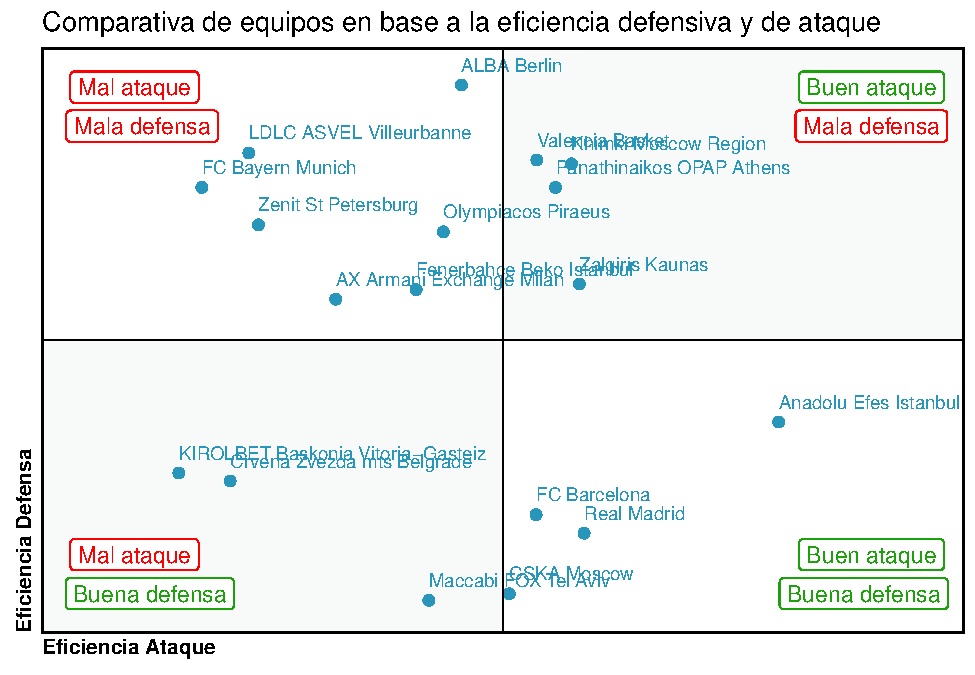
\includegraphics{practica2_files/figure-latex/unnamed-chunk-92-1.pdf}

En la página web de la euroliga tenemos disponible la clasificación de
los equipos hasta la jornada 28, que es la última jornada que se ha
disputado hasta la fecha (31 de mayo de 2020). Se puede acceder a esta
clasificación haciendo
\href{https://www.euroleague.net/main/standings?gamenumber=28\&phasetypecode=RS\&seasoncode=E2019}{\textcolor{blue}{click aquí}}.

A modo de resumen, los primeros puestos son los siguientes:

\begin{longtable}[]{@{}clcccc@{}}
\toprule
\textbf{Posición} & \textbf{Equipo} & \textbf{Victorias} &
\textbf{Derrotas} & \textbf{Pts+} & \textbf{Pts-}\tabularnewline
\midrule
\endhead
1. & Anadolu Efes Istanbul & 24 & 4 & 2432 & 2166\tabularnewline
2. & Real Madrid & 22 & 6 & 2371 & 2165\tabularnewline
3. & FC Barcelona & 22 & 6 & 2357 & 2193\tabularnewline
\bottomrule
\end{longtable}

Y los últimos puestos:

\begin{longtable}[]{@{}clcccc@{}}
\toprule
\textbf{Posición} & \textbf{Equipo} & \textbf{Victorias} &
\textbf{Derrotas} & \textbf{Pts+} & \textbf{Pts-}\tabularnewline
\midrule
\endhead
16. & ALBA Berlin & 9 & 19 & 2304 & 2423\tabularnewline
17. & FC Bayern Munich & 8 & 20 & 2064 & 2281\tabularnewline
18. & Zenit St Petersburg & 8 & 20 & 2055 & 2240\tabularnewline
\bottomrule
\end{longtable}

Si comparamos la posición real en la clasificación con la posición de
cada equipo en el gráfico vemos que queda completamente claro la
relación entre las variables analizadas. Los equipos que están en los
primeros puestos se caracterizan por un buen ataque y una buena defensa
y los equipos que van últimos tienen mala defense y mal ataque.

\newpage

\hypertarget{correlaciones}{%
\subsection{Correlaciones}\label{correlaciones}}

Estos gráficos son complementarios a los presentados en la sección 5.2,
de manera más visual. En probabilidad y estadística, la correlación
indica la fuerza y la dirección de una relación lineal y
proporcionalidad entre dos variables estadísticas. Se considera que dos
variables cuantitativas están correlacionadas cuando los valores de una
de ellas varían sistemáticamente con respecto a los valores homónimos de
la otra: si tenemos dos variables (A y B) existe correlación entre ellas
si al disminuir los valores de A lo hacen también los de B y viceversa.
La correlación entre dos variables no implica, por sí misma, ninguna
relación de causalidad.

\begin{Shaded}
\begin{Highlighting}[]
\KeywordTok{ggcorrplot}\NormalTok{(corr_ataque, }\DataTypeTok{type =} \StringTok{"upper"}\NormalTok{, }\DataTypeTok{lab =} \OtherTok{TRUE}\NormalTok{)}
\end{Highlighting}
\end{Shaded}

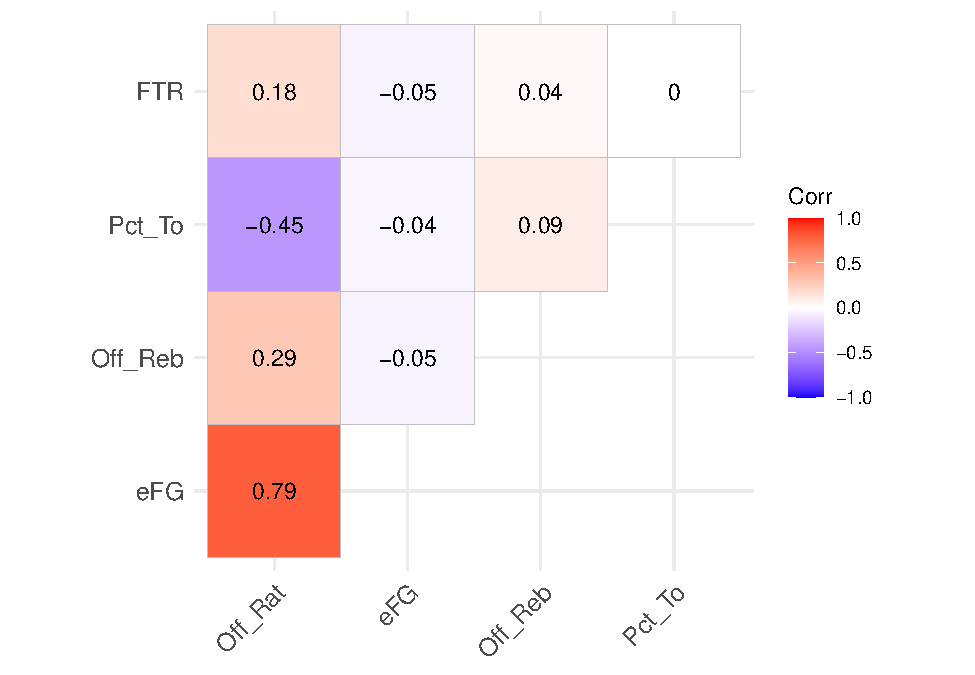
\includegraphics{practica2_files/figure-latex/unnamed-chunk-93-1.pdf}

\begin{Shaded}
\begin{Highlighting}[]
\KeywordTok{ggcorrplot}\NormalTok{(corr_defensa, }\DataTypeTok{type =} \StringTok{"upper"}\NormalTok{, }\DataTypeTok{lab =} \OtherTok{TRUE}\NormalTok{)}
\end{Highlighting}
\end{Shaded}

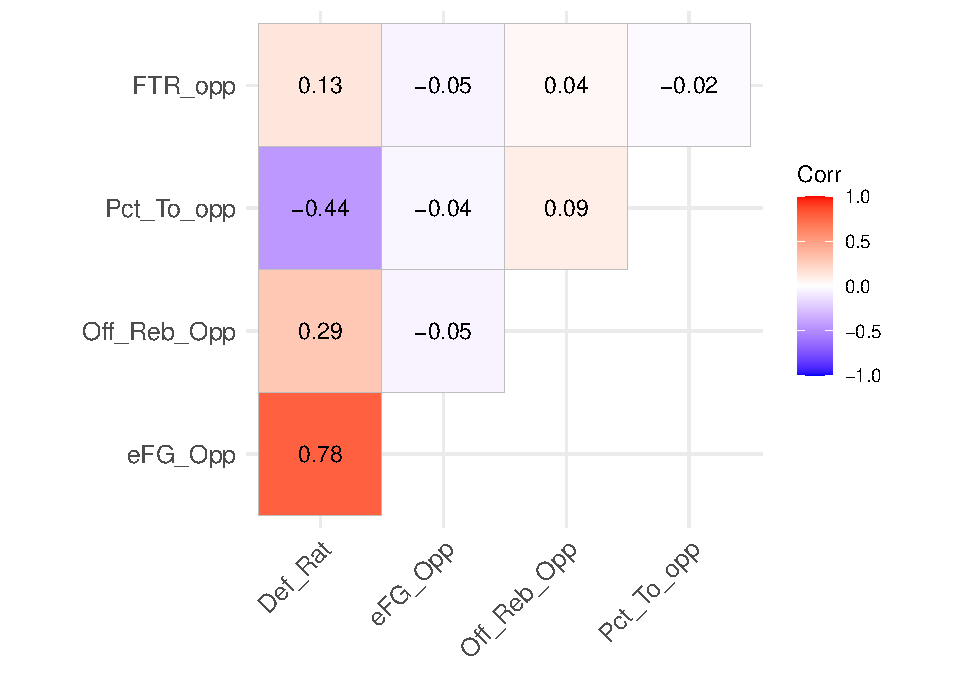
\includegraphics{practica2_files/figure-latex/unnamed-chunk-93-2.pdf}

\newpage

\hypertarget{curva-roc}{%
\subsection{Curva ROC}\label{curva-roc}}

La curva ROC es la representación de la razón o ratio de verdaderos
positivos (VPR = Razón de Verdaderos Positivos) frente a la razón o
ratio de falsos positivos (FPR = Razón de Falsos Positivos) también
según se varía el umbral de discriminación (valor a partir del cual
decidimos que un caso es un positivo). La idea de la curva ROC es que
tenga la mayor área bajo la curva posible y, en general, nos interesa
que la pendiente al principio sea muy elevada para disparar el área de
captura de verdaderos positivos en relación a los errores cuanto antes.

\begin{Shaded}
\begin{Highlighting}[]
\KeywordTok{plot.roc}\NormalTok{( rocobj, }\DataTypeTok{legacy.axes =} \OtherTok{TRUE}\NormalTok{, }\DataTypeTok{print.thres =} \StringTok{"best"}\NormalTok{, }
          \DataTypeTok{print.auc =} \OtherTok{TRUE}\NormalTok{, }\DataTypeTok{auc.polygon =} \OtherTok{FALSE}\NormalTok{, }\DataTypeTok{max.auc.polygon =} \OtherTok{FALSE}\NormalTok{, }
          \DataTypeTok{auc.polygon.col=}\StringTok{"gainsboro"}\NormalTok{, }\DataTypeTok{col =} \DecValTok{2}\NormalTok{, }\DataTypeTok{grid =} \OtherTok{TRUE}\NormalTok{ )}
\end{Highlighting}
\end{Shaded}

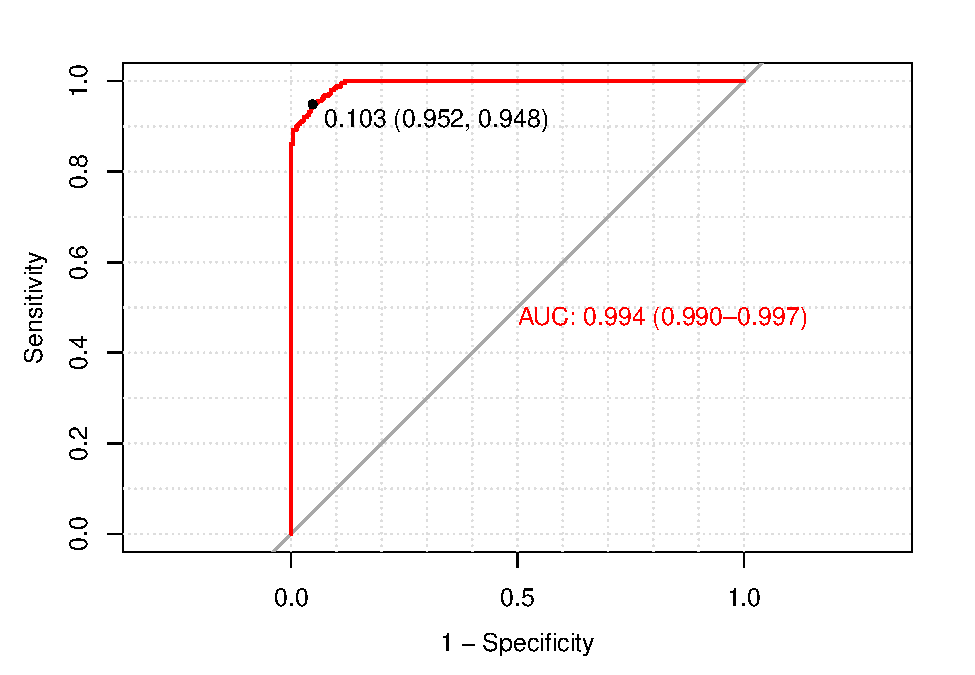
\includegraphics{practica2_files/figure-latex/unnamed-chunk-94-1.pdf}
****

\newpage

\hypertarget{conclusiuxf3n}{%
\section{Conclusión}\label{conclusiuxf3n}}

Como conclusión al trabajo, queríamos destacar: - El Data Science tiene
infinidad de campos a los que contribuir con su crecimiento y el deporte
profesional es uno de ellos, donde además, su uso por lo general apenas
está explotado. - La creación de nuevos estadísticos que depuren los
datos y mejoren la percepción de los mismos, es uno de los puntos donde
se está poniendo el foco. - Uno de los mayores problemas a la hora de
analizar datos del mundo profesional es la mala calidad de las bases de
datos. Somos consciente de que nuestra aproximación es una demostración
de que la Ciencia de Datos puede servir como apoyo al baloncesto pero
que no es realista desde el putno de vista de interpretación. Para ser
más precisos es necesario bases de datos de calidad mayor, en los que se
analice con más detalle los jugadores (veces que botan por derecha o
izquierda), los quintetos con los que juegan (no es lo mismo jugar con
un buen base a la hora de obtener tiros que con un base flojo), los
rivales o el mometno en el que se toman las estad´siticas (es obvio qeu
meter una canasta en los minutos finales o clutch es mucho más valorado
que los jugadores cuyo mejor performance es al principio o en partidos
resueltos). - Hay muchas más métricas de ataque que de defensa, por lo
que es dificil darle el mismo valor a ambos a la hora de realizar
análisis estadísticos. - Las aplicaciones de la Ciencia de datos al
baloncesto son infinitas y de distintas aplicaciones, desde el
entrenador que realiza el scouting y plantea el partido, el que analiza
el resultado y los fallos que se han tenido o incluso la hora de que el
director técnico confeccione el equipo. - Entendemos la ciencia sobre
los datos como un complemento necesario a la hora de tomar decisiones en
el día a día de deporte, pero no como un sustitutivo de las personas. Al
final, siempre que se trabaja con personas hay muchos datos que son
imposibles de medir y que podrían contribuir a la hora, por ejemplo, de
crear tu plantilla en pretemporada. - La dinámica obviamente está
cambiando y el ejemplo de la NBA es el más inmediato, donde todas las
franquicias tienen un equipo de más de treinta personas trabjaando en
Big Data \& Advanced Analytics dando soporte a las decisiones.

\begin{center}\rule{0.5\linewidth}{0.5pt}\end{center}

\hypertarget{contribuciones-al-trabajo}{%
\section{Contribuciones al trabajo}\label{contribuciones-al-trabajo}}

\begin{longtable}[]{@{}lc@{}}
\toprule
\textbf{Contribuciones} & \textbf{Firma}\tabularnewline
\midrule
\endhead
Selección del dataset & MSP, AAG\tabularnewline
Creación del repositorio GitHub & MSP, AAG\tabularnewline
Desarrollo código en R & MSP, AAG\tabularnewline
Redacción de las respuestas & MSP, AAG\tabularnewline
\bottomrule
\end{longtable}

\end{document}
